  % NOTE(cmo): Once upon a time from below \/ but almost entirely customised with
  % very little remaining of original structure.
  % This template was written by John Davies <john.davies@glasgow.ac.uk> 2017-02-06
  % It matches the university specification at the time of writing
  %   for the widths of the page margins and one-and-a-half line spacing
  % You may want to include more packages, particularly for heavy mathematics
  % Please let me know if you find any errors or wish to suggest improvements

% \documentclass[11pt,titlepage,oneside,a4paper]{book}
\documentclass[titlepage,oneside,a4paper,headinclude,
               headheight=16.5pt,footheight=16.5pt,
               chapterprefix,
              %  autoenlargeheadfoot=true,
               parskip=half,
               bibliography=totoc,listof=totoc]{scrbook}
\addtokomafont{disposition}{\rmfamily}
\usepackage{scrlayer-scrpage, datetime}
\usepackage{journals}
\clearpairofpagestyles
\automark{chapter}
\automark*{section}
\cohead{\rightmark}
\ofoot*{\upshape \thepage}
\usepackage{journals}
\usepackage{setspace}
% Set this in the body.
% \setstretch{1.5}
% \onehalfspacing


\usepackage[pdftex]{graphicx}
\usepackage[pdftex]{xcolor}
\graphicspath{{./Figures/}}
% \usepackage{float}
\definecolor{lightGrey}{rgb}{0.9,0.9,0.9}
\definecolor{Red}{rgb}{1.0,0.0,0.0}
% https://personal.sron.nl/~pault/
% Paul Tol's vibrant qualitative colour scheme.
\definecolor{TolBlue}{HTML}{0077BB}
\definecolor{TolCyan}{HTML}{33BBEE}
\definecolor{TolTeal}{HTML}{009988}
\definecolor{TolOrange}{HTML}{EE7733}
\definecolor{TolRed}{HTML}{CC3311}
\definecolor{TolMagenta}{HTML}{EE3377}
\definecolor{TolGrey}{HTML}{BBBBBB}


\definecolor{UniversityBlue}{HTML}{003865}
\definecolor{SkyBlue}{HTML}{005398}

\renewcommand*{\raggedchapter}{\centering}
\renewcommand*{\chapterformat}{%
\color{SkyBlue}%
\rule{0.3\textwidth}{1pt}%
\hspace{0.5em}%
\scalebox{2}{\thechapter}%
\hspace{0.5em}%
\rule{0.3\textwidth}{1pt}%
\vspace*{-0\baselineskip}%
}
\renewcommand*{\sectionformat}{\color{SkyBlue}{\thesection\autodot}\enspace}
\renewcommand*{\subsectionformat}{\color{SkyBlue}{\thesubsection\autodot}\enspace}
\renewcommand*{\subsubsectionformat}{\color{SkyBlue}{\thesubsubsection\autodot}\enspace}

% \usepackage[margin=1em, font=small, labelfont=bf]{caption}
\setcapmargin*{1em}
\setcapindent{1em}
\addtokomafont{caption}{\small}
\addtokomafont{captionlabel}{\bfseries}
% \usepackage{subcaption}
\usepackage{tikz}
\usetikzlibrary{positioning,shapes,fit,arrows,intersections,external,decorations}
\tikzexternalize[prefix=TikzGen/]
\usepackage{pgf}

\usepackage[utf8]{inputenc}
\usepackage[T1]{fontenc}
\usepackage{etoolbox}
% \usepackage{mathpple}
% \usepackage[default,regular,black]{sourceserifpro}
% \usepackage[scaled=0.85]{beramono}
\usepackage{amsfonts,amssymb,amsmath}
\usepackage{bigints}
% \usepackage{fourier}
% \usepackage[charter]{mathdesign}
% \usepackage[notext, nosf, nott]{kpfonts}
\usepackage[default,regular,semibold]{sourceserifpro}

%\usepackage[small, T1]{eulervm}

\usepackage[scale=0.8, semibold]{sourcecodepro}
\usepackage{sourcesanspro}
\usepackage{gensymb}
\usepackage[f]{esvect}
% \usepackage[italic]{mathastext}
% \makeatletter

% \DeclareSymbolFont{EulerLetters}{T1}{zeur}{m}{n}
% NOTE(cmo): This will only work with euler but will replace v in math mode with
% \upsilon, which I personally never use. letters symbol font drawn directly
% from euler.sty
% Don't use this one, see below.
% \DeclareMathSymbol{v}{\mathalpha}{letters}{"1D}
% \DeclareMathSymbol{v}{\mathalpha}{letters}{"1D}

% https://tex.stackexchange.com/q/611645/50104
% Thanks to Ulrike Fischer who found a solution that doesn't break urls. But
% shouldn't be necessary now

% \DeclareMathSymbol{\REALV}{\mathalpha}{letters}{`v}
% \DeclareMathSymbol{v}{\mathalpha}{letters}{"0A}
% \makeatletter
% \appto\UrlSpecials{\do\v{\REALV}}
% \makeatother

% Experiments adjusting characters
%%%%%%%%%%%%%%%%%%%%%%%%%%%%%%%%%%%%%%%%%%%%%%%%%%%%%%%%%%%%%%%%%%%%%%%%%%%%%%%%
% \DeclareSymbolFont{SSFLetters}{OT1}{\sfdefault}{m}{n}
% \DeclareSymbolFont{CMletters}{OML}{cmm}{m}{it}
% https://tex.stackexchange.com/a/27536/50104
% \DeclareFontEncoding{FML}{}{}%
% \DeclareFontSubstitution{FML}{futm}{m}{it}%
% \DeclareSymbolFont{fourier}{FML}{futm}{m}{it}
% \DeclareMathSymbol{\nu}{\mathalpha}{fourier}{23}

% \DeclareMathSymbol{v}{\mathalpha}{fourier}{`v}
% % \DeclareMathSymbol{v}{\mathalpha}{SSFLetters}{`v}
% % \DeclareMathSymbol{\nu}{\mathalpha}{CMletters}{23}
% \DeclareMathSymbol{v}{\mathalpha}{CMletters}{`v}
% \makeatother
% \usepackage{concmath}
%%%%%%%%%%%%%%%%%%%%%%%%%%%%%%%%%%%%%%%%%%%%%%%%%%%%%%%%%%%%%%%%%%%%%%%%%%%%%%%%

\usepackage{lipsum}

%\renewcommand{\mathbf}{\mathbold} %for Eulervm, uses bold instead of bf
% \let\oldhat\hat
% \renewcommand{\vec}[1]{\vv{#1}} %vec uses esvect
% \renewcommand{\hat}[1]{\oldhat{\mathbf{#1}}}
\DeclareMathOperator{\spn}{span}
\DeclareMathOperator{\row}{row}
\DeclareMathOperator{\cols}{col}
\DeclareMathOperator{\nul}{null}
\DeclareMathOperator{\rank}{rank}
\DeclareMathOperator{\nullity}{nullity}
\DeclareMathOperator{\range}{range}
\DeclareMathOperator{\image}{image}
\DeclareMathOperator{\mathion}{ion}
\DeclareRobustCommand{\ion}[2]{\textup{#1\,\textsc{\lowercase{#2}}}}
\newcommand*\element[1][]{%
  \def\aa@element@tr{#1}%
  \aa@element
}
\newcommand{\degr}{\ensuremath{^\circ}}
\newcommand{\arcmin}{\ensuremath{^\prime}}
\newcommand{\arcsec}{\ensuremath{^{\prime\prime}}}
\newcommand{\todo}[1]{\textcolor{red}{#1}}
\newcommand{\tocheck}[1]{\textcolor{orange}{#1}}
\newcommand{\todop}[1]{(\textcolor{red}{#1})}
\newcommand{\tocheckp}[1]{(\textcolor{orange}{#1})}
\newcommand{\citeneeded}{\textcolor{red}{(citation needed)}}


% upquote fixes quotes in verbatim
\usepackage{upquote}
% microtype for the best microtypographical changes (few end-of-line hypenatovs :D)
\usepackage{microtype}

% NOTE(cmo): For university specified _print_ margins and headers
% \usepackage[top=1.8cm,bottom=1.8cm,left=4.0cm,
%             right=1.5cm,headheight=15pt,includeheadfoot]{geometry}
% \usepackage{fancyhdr}
% \pagestyle{fancy}
% \fancyhf{}
% \fancyhead[R]{\nouppercase{\rightmark}}
% \fancyfoot[R]{\thepage}
% \renewcommand{\headrulewidth}{0.2pt}
% \newlength{\quarterPage}
% \setlength{\quarterPage}{7.42cm}
\usepackage[toc,page]{appendix}
\usepackage[UKenglish]{babel}
\usepackage{natbib}

\setcitestyle{authoryear,round,semicolon,aysep={}}

% Add extra non-fragile packages here
\usepackage{siunitx}
\sisetup{mode=text}
% Don't indent paragraphs, separate vertically, KOMA can do this.
% \usepackage{parskip}
% The actual magic
\usepackage{pythontex}
% NOTE(cmo): Swap to deptythontex if you need to use the `depythontex' utility
% to see what code has been generated!
% \usepackage[depythontex]{pythontex}

% NOTE(cmo): Set typearea parameters right at the end
% \setstretch{1.5}
\onehalfspacing
% \KOMAoptions{DIV=12, BCOR=11mm}
% \KOMAoptions{DIV=12, BCOR=16mm}
\newlength{\typeareaoffset}
\setlength{\typeareaoffset}{15pt}
\addtolength{\hoffset}{\typeareaoffset}
\KOMAoptions{DIV=12, BCOR=10mm}
% \usepackage{showframe}

% \usepackage[draft]{changes}
% \newcommand*{\NOTE}[1]{{\color{Red} NOTE: #1}}

\newcommand*{\NOTE}[1]{}

\usepackage{import, url}
\setpythontexcontext{figurewidth=\the\columnwidth}
\newcommand{\includepgf}[1]{\IfFileExists{#1}{\input{#1}}{}}

\usepackage[pdftex,colorlinks=true,bookmarksnumbered=true,linkcolor=UniversityBlue,
  urlcolor=blue,citecolor=UniversityBlue,bookmarksopen=false,pagebackref=true,
  pdfauthor={},pdftitle={},pdfkeywords={},
  pdfsubject={},pdfcreator={},
  pdfproducer={}, pdfencoding=auto, psdextra, breaklinks=true]{hyperref}


\newcommand*{\mgii}{\ion{Mg}{ii}}
\newcommand*{\ha}{H$\alpha$}
\newcommand*{\mghk}{\ion{Mg}{ii}~h\&k}
\newcommand*{\mgiihk}{\ion{Mg}{ii}~h\&k}
\newcommand{\seef}[1]{(see Fig. \ref{#1})}
\newcommand{\figp}[1]{(see Fig. \ref{#1})}
\newcommand{\fig}[1]{Fig. \ref{#1}}
\newcommand{\chap}[1]{Chap. \ref{#1}}
\newcommand{\chapp}[1]{(see Chap. \ref{#1})}
\newcommand{\sect}[1]{Sec. \ref{#1}}
\newcommand{\sectp}[1]{(see Sec. \ref{#1})}
\newcommand*{\kms}{~km~s$^{-1}$}
\newcommand*{\dyncm}{~dyn~cm$^{-2}$}
\newcommand{\comp}[1]{
    {\fontfamily{qcr}\selectfont #1}}
\newcommand{\cgsint}{~erg~s$^{-1}$~cm$^{-2}$~\AA$^{-1}$~sr$^{-1}$}
\newcommand{\cgsintint}{~erg~s$^{-1}$~cm$^{-2}$~sr$^{-1}$}
\newcommand{\eq}[1]{Eq. \ref{#1}}
\newcommand{\eqp}[1]{(see Eq. \ref{#1})}
% Roman or math font derivatives
%\newcommand*{\dd}{\mathrm{d}}
\newcommand*{\dd}{d}
\DeclareSIUnit\erg{erg}
\setcounter{chapter}{0}

\begin{document}
\include{PythonTexSetup}
\begin{titlepage}
\centering
\vspace*{1cm}  % Need the * or the space is swallowed at the top of the page
\bfseries\Large
Diagnostics of the Thermodynamic\\ Properties of Solar Prominences\\
%Thermodynamic Solar Prominence Diagnostics\\
\vspace{2cm}
\normalfont\large{\bfseries{
Aaron W. Peat\\
MSci (Hons)\\
}}
\vspace{1.5cm}
Submitted in fulfilment of the requirements for the\\
degree of Doctor of Philosophy\\
\vspace{1.5cm}
Astronomy and Astrophysics Group\\
School of Physics and Astronomy\\
University of Glasgow\\
\vspace{1cm}

\includegraphics[width=0.5\columnwidth]{GlaLogo.pdf}
\\
\vspace{1cm}
% Insert month and year of date deposited with library for final version
\monthname\hspace{0.2em}\the\year{}
\end{titlepage}
% Order: https://www.gla.ac.uk/media/Media_549236_smxx.pdf Appendix (from MVLS, also not self-consistent on ordering)
\frontmatter  % Turn off chapter numbering, use roman page numbers
% NOTE(cmo): 1.5 spacing in abstract
% \onehalfspacing
% \setstretch{1.5}
% \KOMAoptions{DIV=last}
\include{Misc/Copyright}
\include{Misc/Epigraph}
\include{Misc/Abstract}
% NOTE(cmo): 1.0 spacing for table of contents etc
% \singlespacing
% \KOMAoptions{DIV=last}
\tableofcontents
% \listoftables
\listoffigures
% NOTE(cmo): 1.5 spacing in text
% \onehalfspacing
% \setstretch{1.5}
% \KOMAoptions{DIV=last}

\include{Misc/Acknowledgements}
 
\mainmatter % Turn on chapter numbering, reset page numbers, use arabic
\chapter{Introduction}
\label{Chap:Intro}

The Sun. Without it, we would all be dead. Since the beginning of recorded history, the study of the heavens had been undertaken with an air of caution. Any change in the heavens has often been seen as a frightening omen from a deity or higher power -- the heavens were though to be unchanging and pure. In 1066 the appearance of Halley's comet was seen to be a sign of oncoming misfortune or disaster. The comet is even included on the Bayeux Tapestry, which chronicles the Norman conquest of England. The monks of Canterbury Cathedral witnessed an asteroid impact the Moon in 1178, which was seen as a ominous vision which they were hesitant to disclose. This impact in fact created the Giordano Bruno crater on the northeastern limb of the Moon \citep{sagan_cosmos_1980}. In 1185, Lavrentievsky described the appearance of `horns of which a glow similar to that of red-hot charcoals' during a total solar eclipse \citep{vyssotsky_astronomical_1949}. At the time, this was seen to be a `terrifying sign of the Lord'.

The Sun has been known since the dawn of humankind, yet it remains somewhat of an enigma to this day. This does not mean that the Sun is a complete mystery, however. The Sun has been extensively studied, one of the chief areas of study are of its atmosphere. The Solar atmosphere is said to consist of four layers. The photosphere, the chromosphere, the transition region, and the corona. The photosphere is defined to begin 100~km below the layer of the atmosphere where the plasma becomes opaque to radiation of 5000~\AA\ ($\tau_{500}=1$)\footnote{While it is convention to use Angstroms in Solar Physics, the 500 in $\tau_{500}$ is in nanometres.}. This is defined as such because 5000~\AA\ is approximately the peak wavelength of the blackbody curve of the Sun. We can show this using Wien's Displacement law \eqp{wdl} and an effective Solar surface temperature of 5770~K \citep{woan_cambridge_2000}, 
\begin{equation}
    \lambda=\frac{2.9\times10^{-3}~\mathrm{m~K}}{T}.
    \label{wdl}
\end{equation}
This evaluates to a wavelength of approximately 5026~\AA. The temperature and density structures of the atmosphere appear to be anticorrelated as you journey ever higher in the atmosphere \seef{atmos}. Starting off in the photosphere, temperatures are typically around 5800~K with high pressures of the order of 10$^{5}$~dyn~cm$^{-2}$ \citep{aschwanden_physics_2004}. This gives way to the chromosphere around 525~km above the $\tau_{500}=1$ line, and extends to approximately 2100~km. This gives way to the transition region. This is where the temperature and pressure dramatically rise and fall, respectively. This is only 100~km thick and gives way to the high temperature and low density solar corona \citep{carroll_introduction_2007}. The temperature increase starts at around 5000~K (at the base of the chromosphere \citep{bray_solar_1974}), to over 1~MK in the corona \citep{zirin_solar_1966}. The mechanism behind this heating is not well understood and is known as the coronal heating problem. There have been many proposed mechanisms to drive this heating of which there are two main categories. Alternating current (AC) models and direct current (DC) models. These are described as such due to the electromechanical response to the driver of the heating by the corona. The main separation between these categories is to do with the time scale in which the driver changes the boundary condition. If this is faster than the Alfv\'{e}n transit time, then it is AC. On the other hand, if it is slower, it is DC. Examples of AC includes MHD turbulence and cyclotron resonance, and DC includes reconnection, and turbulence \citep{aschwanden_physics_2004}.

\begin{figure}
    \centering
    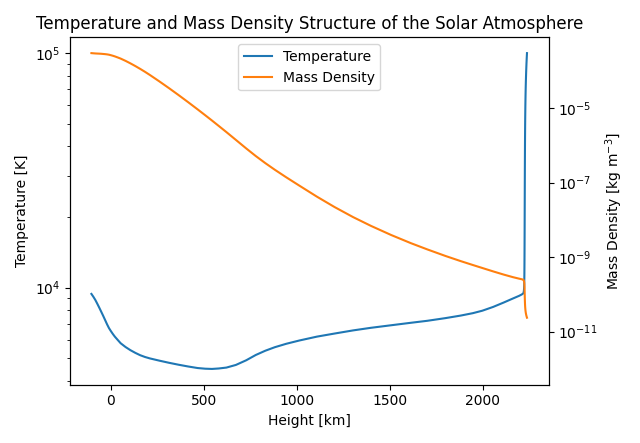
\includegraphics[width=.7\linewidth]{./00Introduction/figs/atmosphere.png}
    \caption[The temperature and pressure structure of the solar atmosphere from the model of \cite{fontenla_energy_1993}]{The temperature and pressure structure of the solar atmosphere from the model of \cite{fontenla_energy_1993}.}
    \label{atmos}
\end{figure}
The temperature and pressure structure of the solar atmosphere up to the base of the transition region can be seen in \fig{atmos}. Meanwhile the layers of the atmosphere can be seen in \fig{layers}. Suspended in the corona are the structures on which this thesis is focused: solar filaments and prominences.
\begin{figure}
    \centering
    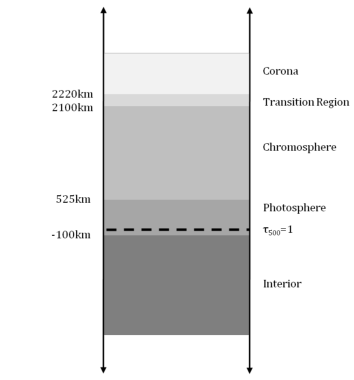
\includegraphics[width=.5\linewidth]{./00Introduction/figs/layers.pdf}
    \caption[A simplified schematic of the Solar atmosphere. Adapted from \cite{carroll_introduction_2007}]{A simplified schematic of the Solar atmosphere. Adapted from \cite{carroll_introduction_2007}.}
    \label{layers}
\end{figure}

\section{Solar Prominences and Filaments}

Solar prominences and filaments are different sides of the same coin. When viewed on disc, they are seen as dark filamentary absorption features and are called filaments. When viewed off-limb, they are seen in emission and called prominences. This distinction is due historical reasons; it was unclear that these structures were one and the same. \fig{both} shows a prominence eruption observation by the Sun-Earth Connection Coronal and Heliospheric Imager \citep[SECCHI; ][]{howard_sun_2008} onboard the Solar Terrestrial Relations Observatory Ahead \citep{driesman_stereo_2008} where it appears both in emission and absorption. The oldest reference to the observation of solar prominences comes from astronomical records in the Russian Chronicles \citep{tandberg-hanssen_solar_1974}. This is the previously mentioned observation made by Lavrentievsky in 1185. These `hot charcoals' to which he refers were very likely solar prominences. Later in 1239, Muratori observed the corona during a solar eclipse and described the corona as having a `burning hole' in it \citep[see ][]{secchi_soleil_1875}. This is also believed to have been a solar prominence \citep{tandberg-hanssen_solar_1974}. It was not until the mid-ninteenth century that serious scientific endeavour was directed towards their study. 
\begin{figure}
    \centering
    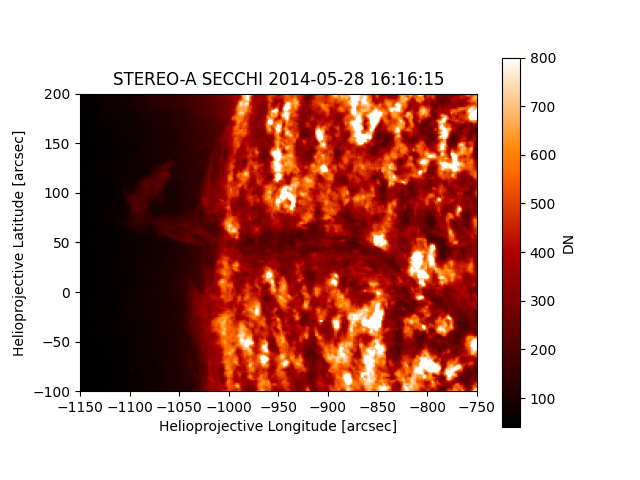
\includegraphics[width=0.7\linewidth]{./00Introduction/figs/prom.png}
    \caption[Prominence observed by the 304~\AA{} filter of STEREO-A/SECCHI]{Prominence observed by the 304~\AA{} filter of STEREO-A/SECCHI. It appears both in emission and absorption. This highlights the similarity and differences between a filament and a prominence.}
    \label{both}
\end{figure}
\subsection{Classification}
There are a number of schemes in which to classify solar prominences. These are based on their morphology, dynamic properties, and general location. Early astronomers realised that prominences in close proximity to active regions were seen to change very rapidly compared to those located in regions of the quiet Sun \citep{vial_solar_2015}. \cite{secchi_soleil_1875} divided solar prominences into three classes; the first two of which we now describe as quiescent and active prominences \citep{tandberg-hanssen_nature_1995}. The third class seems to be a description of what we now know as coronal rain, and the author retracts this third definition later in the text. \cite{secchi_soleil_1875} describes quiescent prominences as peaceful and tranquil. This is a very apt definition. Quiescent prominences tend to form in regions of the quiet Sun away from active regions. They show few motions and only show small changes over hours and/or days. These are very stable and persists from days to weeks. Additionally they are unlikely to erupt unless there is some trigger nearby, such as a flare or CME. This, however, does not mean that they are not dynamic, they are just less so than their counterparts. Active prominences tend to form in active regions and are less stable and far more dynamic than their calmer siblings. Due to the greater magnetic field in the active regions where they form, they tend to be much smaller and shorter lived. They are much more prone to spontaneous eruption than their siblings.Secchi goes on to further subdivide these main classes into subclasses comprising of clouds, filaments, stems, plumes, horns, cyclones, flames, jets, sheafs, and spikes. Presently the distinction between these subclasses is not clear and the main two categories are instead used without these subclasses.

\subsection{Formation}

There are two leading ideas about how prominences form. On one hand, many believe that some prominences form due to condensation of hot material from the corona. This approach is applied to both active and quiescent prominences. On the other hand, some prominences are believed to have photospheric or chromospheric origins, with active prominences being lifted up and out of these layers \citep{tandberg-hanssen_nature_1995}. However, all prominences form in filament channels which form around polarity inversion lines \citep[PILs; ][]{vial_solar_2015} -- regions where the photospheric magnetic field flips polarity. A filament channel forms when chromospheric fibrils align themselves with the PIL. Additionally, prominences can only form in these regions where no fibrils cross the PIL \citep{martin_conditions_1998}. The mechanism which causes these fibrils to align themselves with the polarity inversion line is not well understood and many processes to describe this phenomena have been suggested. One such suggestion is that of the submergence and cancellation of the transverse magnetic field component, leaving the axial field component behind \citep{martin_conditions_1998, wang_formation_2007}. Alternatively, it has been suggested that strong shearing motions in the photospheric plasma localised to the PIL are responsible \citep{devore_dynamical_2000}. The former may be supported by \cite{wang_transient_2013}, where they observed transient brightenings along a filament channel, which they suggest are associated with flux cancellation. The latter was explored by \cite{hindman_helioseismically_2006} where sheared flows of the order of 30\kms{} were observed to either side of a PIL. Filament channels often form with magnetic arcades, closed field lines which pass high and over the channel, anchored in regions of opposing polarity on either side of the channel. When a prominence forms in the channel, this arcade is seen to exist above both. Between the prominence and the arcade one can observe a dark coronal cavity \citep{tandberg-hanssen_nature_1995}.

\subsection{Main Components}
Prominence are seen to have two main observable features, their horizontal spine which is suspended above the solar surface, and barbs which anchor the spine to the solar surface. Barbs are very easily seen in coronal filters, such as 171~\AA{} from the Atmospheric Imaging Assembly \citep[AIA; ][]{lemen_atmospheric_2012} onboard the Solar Dynamics Observatory \citep[SDO;][see \fig{threestages}]{pesnell_solar_2012}. These features are more readily identifiable as filaments on the disc as their orientation lends well to being observed.
Another important feature of a prominence is the prominence to corona transition region \citep[PCTR; ][]{vial_solar_2015}. This is analogous to the transition region (TR) of the classic view of the solar atmosphere. Here the prominence transitions from cool photospheric and chromospheric temperatures ($\sim6000$~K) to that of coronal temperatures ($>500~000$~K). Additionally the PCTR also includes a pressure gradient (like the TR) to smoothly transition from a high pressure prominence to the more tenuous corona. As such prominences are seen to emit spectral lines of a wide range of elements. Prominences are known to be primarily composed of hydrogen and are routinely observed in H$\alpha$, with many stations around the world observing the Sun in this wavelength daily\footnote{such as https://bass2000.obspm.fr or https://gong2.nso.edu}. However, we can also observe line profiles which form at much higher temperatures, such as \mgiihk, which is the main focus of this work. This temperature and pressure gradient makes solar prominences appear more extended in ultraviolet compared to H$\alpha$ \citep{heinzel_why_2001}. When the PCTR is taken into account when modelling solar prominences, we find that we achieve a better match between observed and synthetic spectra \sectp{Chap:prom} which highlights the impact that it has on line formation in the prominence.

\subsection{Thermodynamics and General Properties}


Prominences are comprised of cool dense plasma suspended in the hot and tenuous solar corona \citep{labrosse_physics_2010}. Due to their structure, as discussed in the previous section, it is easy to see that prominences comprise of a wide range of temperatures and pressures. The core of a prominence tends to be the coolest part of the prominence, with temperatures of the order of $10^4$~K. However, the PCTR reaches much higher temperatures, of the order of $10^4-10^6$~K. The densities observed show the inverse of this, as one familiar with the TR would expect. The core of a prominence has electron densities between $10^9-10^11$~cm$^{-3}$, but this drops to $10^6-10^8$~cm$^{-3}$ in the PCTR. Pressures show a similar story with the core exhibiting pressures of the order of $0.02-1$~dyn~cm$^{-2}$ and the PCTR with $0.2$~dyn~cm$^{-2}$. It is possible for the PCTR to experience higher pressures than some internal pressures. Along with their thermodynamic properties, they also exhibit a range of motions. Fine motions within the prominence itself can be of the order of $3-20$\kms{} in the core of the prominence, up to 30\kms{}. These `microturbulent' velocities are responsible for widening the line profiles we observe from prominences. However, these are not bulk flows that can be observed directly and must be inferred from the line profiles. Bulk flows tend to be much smaller, reaching 5\kms{} in the core of the prominence and 10\kms{} in the PCTR \citep{labrosse_physics_2010}. When these flows move away from the solar surface, the radiation is subject to Doppler dimming. Any incident radiation from the solar disc arriving at the prominence is seen to be Doppler shifted by the prominence. This causes less radiation to be absorbed and scattered as the radiation arriving at the prominence is shifted relative to the absorption profile. Line profiles will be seen to be less intense than their static counterparts. 

\subsection{Magnetic Field Strength}

The magnetic field strength of a solar prominence is difficult to determine and requires some measurement of the Stokes parameters. The Stokes parameters consist of four vectors, I, Q, U, and V. I is the intensity of the observed radiation, this does not measure polarisation. Q and U measure the linear polarisation of the light. Q and U are separated by 45\degr{} such that a better measure of the polarisation can be made. V measures the circular polarisation of the light, giving $1$ and $-1$ for fully right hand polarised and left hand polarised light, respectively \citep{toro_iniesta_introduction_2007}.
The magnetic field in a prominence is typically quoted as being on the order of 1s to 10s of Gauss \citep{tandberg-hanssen_nature_1995}. Quiescent prominences have been measured to have magnetic fields of $3-15$~G, while active prominences have been observed with magnetic fields of $30-45$~G \citep{mackay_physics_2010}.



\subsection{Eruptions and Demise}

Prominences boast a range of lifetimes. This depends on whether it is a quiescent or active prominence.
It is generally accepted that instabilities lead to the demise of prominences. The source of these instabilities, however, is debated. There are two main equilibria responsible for the stability of solar prominences; thermal equilibrium and magnetohydrostatic equilibrium \citep{tandberg-hanssen_nature_1995}. The breakdown of either of these will lead to the death of a prominence. One of the more dramatic of these, is a prominence eruption. This is the expulsion of a prominence from the Sun. The most energetic of these %which reach the solar escape velocity ($v_{esc}=617.7$\kms)
are called flare sprays \citep{tandberg-hanssen_solar_1974} and are closely related to coronal mass ejections (CMEs). Prominence cores are frequently viewed as the central core of a CME in white light coronagraphs \citep{vial_solar_2015}. One model which attempts to explain the eruption of solar prominences is that of mass draining by \cite{jenkins_modeling_2019}. The authors argued that mass draining causes an instability which leads to a rise in height of the prominence. This height increase then continues until the prominence erupts or becomes completely devoid of material through draining. Which of these two fates the prominence meets depend on the conditions it is under before the draining commences. \cite{wang_transient_2013} observed brightenings at the end points of erupting filament channels in the 195~\AA{} filter of the Extreme-Ultraviolet Imaging Telescope \citep[EIT; ][]{delaboudiniere_eit_1995} onboard the Solar and Heliospheric Observatory \citep[SOHO; ][]{domingo_soho_1995}. These were interpreted to be sites of magnetic reconnection catalysed by the rise of the host magnetic field lines host to the prominence. This rise is then said to have crossed into the overlying coronal loops and reconnected with them, further accelerating the eruption via the breakdown of magnetohydrostatic equilibrium. When a quiescent prominence erupts, the source filament channel remains. This can then go on to have another prominence form in the vacant channel, starting the whole process again \citep{vial_solar_2015}. If the thermal equilibrium breaks down, the prominence can quickly heat up to coronal temperatures and effectively evaporate. Prominences lose energy by radiation, since radiative losses are proportional to the square of the density, this shows that it is an effective way to quickly dissipate radiation. If the thermal losses are too small, however, the prominence will quickly heat up. This breakdown and heating of the prominences happens on the order of seconds to minutes \citep{tandberg-hanssen_nature_1995}.

\section{Magnesium}
Magnesium is one of the most abundant elements in the solar atmosphere. Therefore its singly ionised state, \mgii{}, has great diagnostic potential \citep{leenaarts_formation_2013-1}. It is clear that once ionised magnesium, \mgii{}, is a very important ion. Its principle transitions, \mgiihk{}, form in the upper chromosphere and lower transition region \citep{depontieu_interface_2014}. This formation region will capture the hotter parts of the prominence, and gives us insight into the nature of the PCTR. The rest wavelengths of the \mgiihk{} lines are 2803.53~\AA{} and 2796.35~\AA, respectively \citep{levens_modelling_2019}. The features of the \mgiihk{} lines are usually separated into five distinct features per line. The violet features $1_\text{v}$ and $2_\text{v}$ are the points at which the wings of the emission start to increase, and when its peak violet intensity is reached, respectively. The red features, $1_\text{r}$ and $2_\text{r}$, are described similarly.
\begin{figure}
    \centering
    \includegraphics*[width=0.8\linewidth]{./00Introduction/figs/mgii.png}
    \caption{The spectral features of the \mgiihk{} lines. This spectrum was taken from the edge of the solar disc on 2018-04-19.}
    \label{fig:mgiifeatures}
\end{figure}
However, the feature labelled $3$ in \fig{fig:mgiifeatures} is the central reversal and line core. In general, the optical thickness of \mgiihk{} is such that many of its observed line profiles exhibit a central reversal. This is encapsulated by Eq. \ref{eq:line}; $\tau_\lambda$ is a function of wavelength, and in the case of \mgiihk{} $\tau_\lambda$ is largest towards the line core, and it is lowest towards the wings. This means that the line core tells us more about the surface of the plasma, but the wings allow us to see deeper into the structure. This is also the reason for the appearance of this double peak. However, there needs to be a sufficient amount of material to absorb enough of the line core for the line to manifest with a self reversal. This is because $\tau_\lambda$ is also a function of distance through the material. In solar prominences, in general we do not see this double peaked behaviour. When a line presents itself in this single peaked fashion, the $2_v$ and $2_r$ features are not present. It was shown by \cite{heinzel_formation_2014} that the \mgiihk{} line cores are very sensitive to the temperature structure in the PCTR, highlighting their diagnostic potential to explore this region. 


\section{A Brief Foray into Radiative Transfer}
Radiative Transfer is the study of how electromagnetic radiation moves through and interacts with a medium. As put by \cite{hubeny_theory_2015}, `The radiation we receive from a star contains an enormous wealth of information about the structure and composition of its atmosphere.' This should be motivation enough on its own to study this extremely interesting field. Disregarding magnetic complexities, there are  five main processes which govern the solar spectra that we observe; bound-free (bf) interactions, where atoms are ionised and recombine liberating a photon in the process; free-free (ff) interactions, where electrons collide with ionised nuclei causing a photon to be emitted due to the energy lost by the electron; bound-bound (bb) interactions, where electrons move from one energy level to another within the same atom; and Rayleigh and Thomson scattering, where the former concerns photons scattering from neutral hydrogen, and the latter, photons scattering from free electrons \citep{rutten_introduction_1993}. The radiation received from an emitting medium can be represented by the specific intensity,
\begin{equation}
    \frac{\dd I_\lambda}{\dd s}=j_\lambda-\chi_\lambda I_\lambda,
    \label{eq:1}
\end{equation}
where $j_\lambda$ is the monochromatic emissivity, $\chi_\lambda$ is the linear extinction coefficient, and $s$ is the path length of the beam. Kirchoff's Law which defines the source function $S_\lambda$ is also important \citep{woan_cambridge_2000},
\begin{equation}
    S_\lambda\equiv\frac{j_\lambda}{\chi_\lambda}.
\end{equation}
This describes the energy of new photons entering the beam, and is normalised by the linear extinction coefficient which describes the extinction of the radiation as it travels through the medium. $\chi_\lambda$ is related to the optical path length by,
\begin{equation}
    \dd\tau_\lambda(s)=\chi_\lambda(s)\dd s.
    \label{eq:3}
\end{equation}
This allows us to define the optical thickness as,
\begin{equation}
    \tau_\lambda(D)=\int_0^D\chi_\lambda(s)\dd s,
\end{equation}
where $D$ is the path length through the material. Combining Eqs. \ref{eq:1} and \ref{eq:3} allows us to change variables from $s$ to $\tau_\lambda$ such that,
\begin{equation}
    \frac{\dd I_\lambda}{\dd \tau_\lambda}=S_\lambda-I_\lambda.
\end{equation}
Then multiplying through by $\exp(\tau_\lambda(D))$ and integrating between 0 and $\tau_\lambda(D)$ we get,
\begin{equation}
    I_\lambda(\tau_\lambda)=I_\lambda(0)\exp(-\tau_\lambda)+\int_0^{\tau_\lambda}S_\lambda(t_\lambda)\exp(-(\tau_\lambda-t_\lambda))\dd t_\lambda.
\end{equation}
$\tau_\lambda$ is implicitly a function of distance here. $t_\lambda$ describes the path length in terms of optical depth. If we assume that the source function is constant across $t_\lambda$, we can evaluate this integral and change variables such that,
\begin{equation}
    I_\lambda(D)=I_\lambda(0)\exp(-\tau_\lambda)+
    \overline{S_\lambda}\left(1-\exp\left(-\tau_\lambda\right)\right),
    \label{eq:line}
\end{equation}
and what we have is the formal solution to the radiative transfer equation. $I_\lambda(0)$ is the radiation entering the material, and $\overline{S_\lambda}\left(1-\exp\left(-\tau_\lambda\right)\right)$ describes the radiation created by the material that can reach $D$, and $I_\lambda(D)$ is the total radiation at $D$ given that $\tau_\lambda=\tau_\lambda(D)$. In local thermodynamic equilibrium (LTE) the source function becomes the Planck function, $B_\lambda$, such that \citep{rutten_introduction_1993,hubeny_theory_2015},
\begin{equation}
    I_\lambda(D)=I_\lambda(0)\exp(-\tau_\lambda)+
    B_\lambda\left(1-\exp\left(-\tau_\lambda\right)\right).
\end{equation}
If there is a coherent and isotropic scattering term, the source function is modified to become \citep{hubeny_theory_2015}, 
\begin{equation}
    S_\lambda=\epsilon_\lambda B_\lambda+(1-\epsilon_\lambda)J_\lambda,
\end{equation}
where $\epsilon$ is the thermal coupling parameter or destruction probability, and $J_\lambda$ is the mean intensity of radiation, ie the mean of the specific intensity over all solid angles. If the reader wishes, $\lambda$ may be substituted for $\nu$ in any of these equations.
This powerful set of equations can help us to model the radiation that comes from the solar atmosphere to better understand how the radiation we see from the Sun is formed.

For a simple 2-level atom, the source function takes the form of \citep{hubeny_theory_2015,levens_diagnostics_2018},
\begin{equation}
    S_{lu}=\frac{n_uA_{ul}}{n_lB_{lu}-n_uB_{ul}}\frac{\psi_{ul}(\lambda)}{\phi_{lu}(\lambda)}
\end{equation}
Where $A$ and $B$ are the Einstein coefficients. $A_{ul}$ denotes spontaneous emission, $B_{ul}$ denotes stimulated emission, and $B_{lu}$ denotes absorption. $n_u$ is the population of the upper level, $n_l$ is the population of the lower level. $\psi_{ul}(\lambda)$ is the emission profile and ${\phi_{lu}(\lambda)}$ is the absorption profile. In complete redistribution (CRD), it assumed that there are enough collisions in the plasma such that when a photon is absorbed by an atom, the atom relaxes such that the photon is re-emitted anywhere in the line. That is to say, that $\psi_{ul}(\lambda)$=${\phi_{lu}(\lambda)}$. On the opposite end of this is scattering, where an absorbed photon is re-emitted at its original wavelength and its not redistributed along the line. Partial redistribution (PRD) is a combination of these two regimes. The photon is more likely to be re-emitted at a small range of frequencies around its original frequency. In the CRD approximation, the source function becomes,
\begin{equation}
    S_{lu}\approx\frac{n_uA_{ul}}{n_lB_{lu}-n_uB_{ul}}
\end{equation}
However, as shown by \cite{milkey_resonance_1974}, this does not hold in the optically thick regime. This includes ions such as \mgii. Under non-LTE conditions, the source function varies from the Planck function. This cannot be solved analytically and must be solved numerically. This is because the source function is strongly dependent on the radiation field \citep{labrosse_physics_2010}. Careful consideration of the level populations and radiation field is required to find the source function. The equations of statistical equilibrium are used to achieve this \citep{labrosse_physics_2010},
\begin{equation}
    \frac{dn_i}{dt}=\sum_{j\neq i} n_j\left(R_{ji}+C_{ji}\right)-n_i\sum_{j\neq i} \left(R_{ij}+C_{ij}\right)
\end{equation}
\begin{equation}
    \frac{dn_i}{dt}=\frac{\partial n_i}{\partial t}+\frac{\partial n_iV}{\partial x}
\end{equation}
Like before, $n_i$ is the population of the ith level, and $n_j$ is the population of the jth level. V is the flow velocity. $C_{ij}$ and $C_{ji}$ are the collisional rates which are proportional to the electron density ($n_e$). $R_{ij}$ and $R_{ji}$ are the radiative rates for absorption and stimulated emission. These depend on the radiation field of the line and continuum.  For a simple two level atom like before, the equations of statistical equilibrium can be simply written as \citep[ignoring the time and velocity terms,][]{labrosse_physics_2010},
\begin{equation}
    n_lB_{lu}\overline{J}_{lu}+n_lC_{lu}=n_uA_{ul}+n_uB_{ul}\overline{J}_{lu}+n_uC_{ul}
\end{equation}

\section{Radiative Transfer Code}

Recently, there has been 3D prominence modelling efforts by \citep{gunar_3d_2015}. They employ, what they name, 3D whole-prominence fine structure (WPFS) modelling. Where they model a 3D magnetic field using the 3D non-linear force-free (NLFF) simulations of \cite{mackay_non-linear_2009}, in which they identify dips or hammocks which they then allow to fill with plasma. This geometry is then used as the configuration for radiative transfer simulations. The study shows the importance of the projection effect and naturally reproduces fine structure emission. While this method is very powerful, the authors have little control over the geometry of the simulation like we do in more conventional approaches. Both methods have their pros and cons, but this WPFS modelling is still quite new with a lot of potential. While it is possible to use it to simulate a prominence if we know the underlying magnetic field, it may also be possible to infer the magnetic field structure if we start with an observation of a prominence and work backwards. 

In this thesis, we use two radiative transfer codes to solve them numerically. We first introduce the 1D non-local thermodynamic equilibrium (NLTE) RT code, PROM. Later introducing the 2D NLTE RT code, RTCY.

\subsection{PROM}
\label{promintro}
\begin{figure}
    \centering
    \includegraphics*[]{./02Modelling1D/figs/20180419/prom.png}
    \caption[Construction of the simulation in PROM. Based on \cite{gouttebroze_formation_1997} and \cite{labrosse_effect_2007}.]{Construction of the simulation in PROM. The curvature of the Sun is exaggerated in this cartoon. Based on \cite{gouttebroze_formation_1997} and \cite{labrosse_effect_2007}.}
    \label{promsetup}
\end{figure}
\cite{gouttebroze_hydrogen_1993} and \cite{heinzel_theoretical_1994} introduced the 1D radiative transfer code, PROM. PROM solves the set of radiative transfer equations to produce symmetrical (around the line core) line profiles. In its initial implementation, it only produced hydrogen spectra. The lines exhibited in \cite{gouttebroze_hydrogen_1993} were Ly$\alpha$, Ly$\beta$, H$\alpha$, Ly$\gamma$, H$\beta$, and P$\alpha$ -- the first six bound-bound neutral hydrogen transitions. In theory, any bound-bound line produced by a twenty level hydrogen atom could be output from PROM. Additionally, the bound-free transition of the Lyman continuum is included. This aimed to improve on the work by \cite{heasley_theoretical_1974} where the authors adapted NLTE code to the problem of an illuminated slab/prominence. Throughout the years, many modifications have been made to PROM; \cite{gouttebroze_formation_1997} and \cite{gouttebroze_calcium_2002} introduced the \ion{Ca}{ii} lines. Here, a five level \ion{Ca}{ii} ion is implemented, with an additional level for unionised (\ion{Ca}{i}) and twice ionised (\ion{Ca}{iii}), respectively. This allowed for the modelling of the \ion{Ca}{ii}~H\&K lines. \cite{labrosse_formation_2001} introduced the \ion{He}{i} and \ion{He}{ii} lines, with a 33 level (plus continuum) atom for both \ion{He}{i} and \ion{He}{ii}. \cite{labrosse_nonlte_2004} introduced the prominence-to-corona transition region (PCTR) as formulated in \cite{anzer_energy_1999}. The PCTR takes the form of a pressure ($p$) and temperature ($T$) gradient as a function of column mass, $m$. 
\begin{equation} 
    T(m)=T_{\text{cen}}+(T_{\text{tr}}-T_{\text{cen}})\left(1-4\frac{m}{M}\left(1-\frac{m}{M}\right)\right)^\gamma
    \label{tstrat}
\end{equation}
\begin{equation}
    p(m)=4p_c\frac{m}{M}\left(1-\frac{m}{M}\right)+p_{\text{tr}},
    \label{pstrat}
\end{equation}
where,
\begin{equation}
    p_c=\frac{{B_{z_0}}^2}{8\pi}=p_{\text{cen}}-p_{\text{tr}},
    \label{pcdef}
\end{equation}

where $M$ is the total column mass, $\frac{M}{2}$ is the centre of the prominence, $B_{z_0}$ is magnetic field perpendicular to the solar surface, $T_{\text{cen}}$ and $p_{\text{cen}}$ are the central temperature and pressure respectively, and $T_{\text{tr}}$ and $p_{\text{tr}}$ are the temperature and pressure at the outer edge of the PCTR respectively. These equations \citep{anzer_prominence_1998, anzer_energy_1999,labrosse_nonlte_2004} allow the core of the prominence to gently transition to the corona without discontinuity. The value of $\gamma$ is strictly more than 0. If $\gamma=0$, the prominence becomes isothermal with a temperature of that of the corona, while the pressure still gradually changes. A prominence of such conditions is not possible in nature. \cite{levens_modelling_2019} builds on the \ion{Ca}{ii} formulation from \cite{gouttebroze_formation_1997} to introduce a five level (plus continuum) \mgii{} ion to produce the \ion{Mg}{ii}~h\&k lines (2803.53~\AA\ and 2796.35~\AA) and the \ion{Mg}{ii} triplet lines (2791.60~\AA, 2798.75~\AA, and 2798.82~\AA). When modelling these lines, it must be considered whether CRD or PRD is used.  It was shown by \cite{milkey_resonance_1974} that PRD is important when modelling the \mgii{} resonance lines, and so partial redistribution (PRD) is used here. The incident \mgii{} radiation is taken from near disc centre spectroscopic \ion{Mg}{ii} observations from the Interface Region Imaging Spectrograph \citep[IRIS;][]{depontieu_interface_2014}.
\begin{figure}
    \centering
    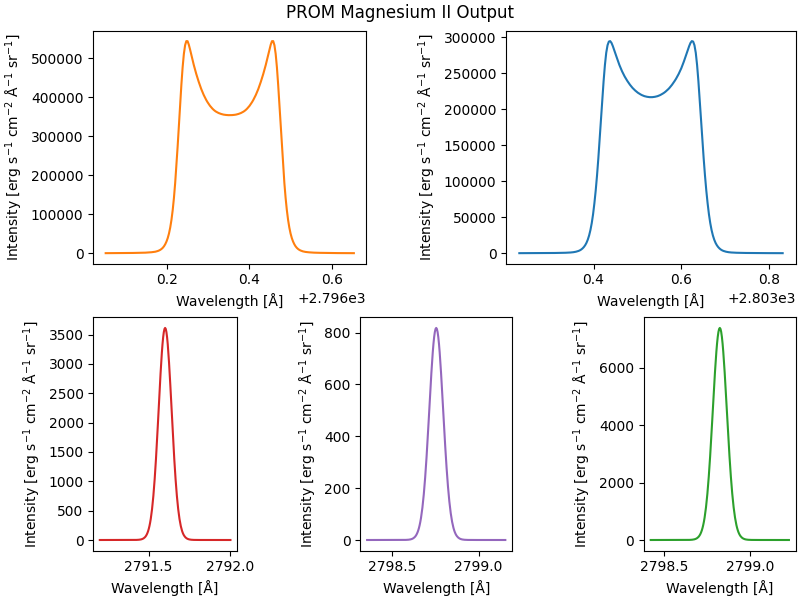
\includegraphics[width=0.9\linewidth]{./02Modelling1D/figs/20180419/promexample2.png}
    \caption[An example of the magnesium output from PROM.]{An example of the magnesium output from PROM. The top panels are \mgiihk{}, respectively, while the bottom panels are the \mgii{} triplet lines. The parameters of this model are; $T_\text{cen}=8000~$K, $T_\text{tr}=100000~$K, $p_\text{c}=0.5~$dyn$~$cm$^{-2}$, $p_\text{tr}=0.01~$dyn$~$cm$^{-2}$, $\gamma=5$, $v_T=5~$km$~$s$^{-1}$, $H=10~$Mm, and $v_{rad}=0~$km$~$s$^{-1}$.}
    \label{promexample}
\end{figure}

Within PROM, prominences are represented by a semi-infinite plane parallel slab perpendicular to the solar surface. This slab is illuminated on both sides by the angle-averaged incident intensity. A schematic diagram can be seen in Fig. \ref{promsetup}. PROM (with a PCTR) has several input parameters. surface temperature, the temperature at the edge of the PCTR ($T_{\text{tr}}$ in \eq{tstrat}); central temperature, the temperature in the core of the prominence ($T_{\text{cen}}$ in \eq{tstrat}); surface pressure, the pressure at the edge of the PCTR ($p_{\text{tr}}$ in \eq{pstrat}); central gas pressure, the central gas temperature of the prominence ($p_{\text{c}}$ in eqs. \ref{pstrat} and \ref{pcdef}); thickness, the geometric width of the prominence along the line of sight ($L$ in Fig. \ref{promsetup}); column mass, the mass as a function of distance through the prominence; $\gamma$, a dimensionless number which dictates the extent of the PCTR; microturbulent velocity, the unresolved stochastic motions within the prominence; altitude, the height above the solar surface ($H$ in Fig. \ref{promsetup}); and radial velocity, bulk velocity away (when positive) or towards (when negative) from the Solar surface ($v_\text{rad}$ in Fig. \ref{promsetup}). The outputs are the intensities of the considered line profiles, the number density of the considered species, their level populations, and the optical thickness of the line core. An example of the \mgii\ line profiles output from a run of PROM from \cite{levens_modelling_2019} can be seen in Fig. \ref{promexample}. The spectral resolution of these simulated line profiles is 3~m\AA, much greater than any current instrument.

\subsection{RTCY}
\label{rtcyintro}
Radiatif Transfert Cylindrique (Cylindrical Radiative Transfer; RTCY) was developed over a series of seven papers \citep{gouttebroze_radiative_2004,gouttebroze_radiative_2005,gouttebroze_radiative_2006,gouttebroze_radiative_2007, gouttebroze_radiative_2008, gouttebroze_radiative_2009,labrosse_radiative_2016}. The prominence is modelled as a cylinder suspended above the solar surface with a set of thermodynamic, geometric, and dynamic properties. Currently, this model is isobaric. However, it is possible to include a PCTR for the temperature gradient. The implementation of the geometric and dynamic properties can be seen in \fig{fig:rtcyv5}. 
\begin{figure}
    \centering
    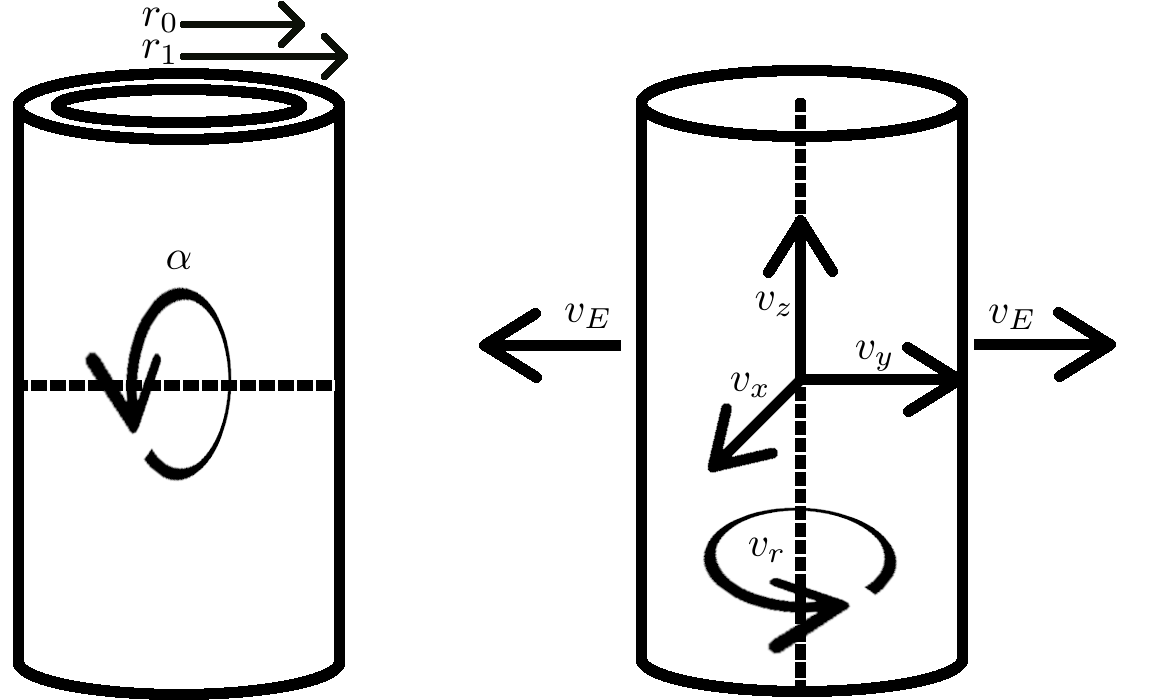
\includegraphics[width=0.71\linewidth]{./03Modelling2D/figs/rtcy.png}
    \caption[The prominence model employed by RTCY.]{The prominence model employed by RTCY. The observer is looking from the right to the left and the Solar surface is parallel to the bottom of the page. \textit{Left}: The geometric properties of the prominence model.  \textit{Right}: The velocity settings of the model. The $v_E$ arrows should be placed all around the circumference of the cylinder, but are omitted for clarity. Please note that $x$ is out of the page.}
    \label{fig:rtcyv5}
\end{figure}
\begin{figure}
    \centering
    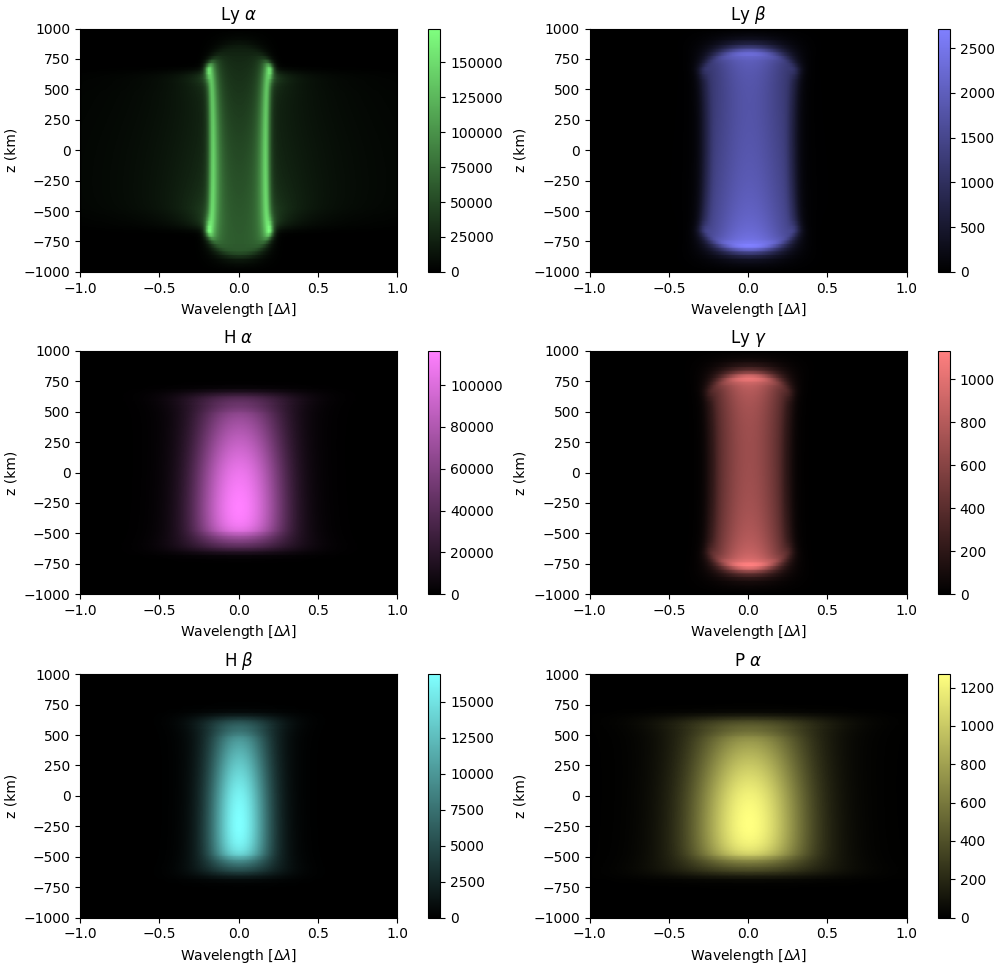
\includegraphics[width=\linewidth]{./03Modelling2D/figs/exh.png}
    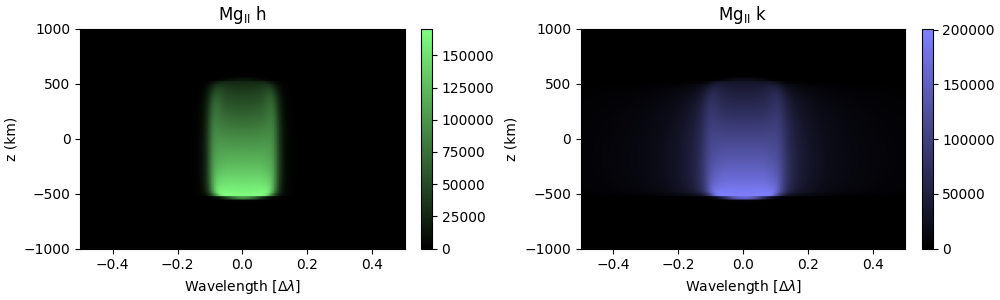
\includegraphics[width=\linewidth]{./03Modelling2D/figs/exmg.png}
    \caption[Example of the output of RTCY for the principal neutral hydrogen transitions and the h\&k lines of once-ionised magnesium.]{Example of the output of RTCY for the principal neutral hydrogen transitions and the h\&k lines of once-ionised magnesium. The units of the colourbars are \cgsint. The parameters of this example run are; $P=0.1$~dyn~cm$^{-2}$, $r_0=500$~km, $r_1=1000$~km, $T_0=6000$~K, $T_1=100~000$~K, $v_T=5$~km~s$^{-1}$, $\alpha=\frac{\pi}{2}$~rad and $H=10000$~km with no velocity setting active.}
    \label{fig:introexhmg}
\end{figure}
For the geometric properties, $r_0$ is the radius for which the cylinder is isothermal in km; $r_1$ is the radius of the PCTR in km; and $\alpha$ is the rotation of the cylinder, where $\alpha\in[0,\frac{\pi}{2}]$ due to symmetry. Not included on this diagram is $H$, the height above the solar surface in km. 
The thermodynamic properties include the gas pressure ($P$) in dyn~cm$^{-2}$; temperature in the core of the prominence ($T_0$) in K; temperature of the PCTR ($T_1$) in K; and the microturbulent velocity within the prominence ($v_T$) in km~s$^{-1}$. RTCY also has an isothermal and isobaric mode, where $T_0$ and $T_1$ are replaced by a single temperature, $T$, and $r_0$ and $r_1$ are replaced by a single diameter, $D$.
There are three main velocity settings; $v_x$, $v_y$, and $v_z$ which make up the translation velocity setting in km~s$^{-1}$; $v_E$ is the expansion velocity setting in km~s$^{-1}$ where the whole prominence expands radially outward from the axis of rotational symmetry; and $v_r$ is the rotational velocity setting in rad~s$^{-1}$. These settings can only be run independently of one another due to the way velocities are currently implemented. If more than one of these is specified in the run parameters, the expansion velocity setting takes precedence, followed by the rotational velocity setting, and finally the translational velocity setting has the lowest precedence. 
The code simulates the emission that would be seen by a single slit of a hypothetical spectrometer aligned along $z$. The version of the code employed here simulates hydrogen and magnesium emission. By default, it produces the Ly$\alpha$, Ly$\beta$, H$\alpha$, Ly$\gamma$, H$\beta$, P$\alpha$; and \mgii{}~h and \mgii{}~k lines. This code uses Complete Redistribution (CRD) for these resonance lines. See \fig{fig:exhmg} for an example of the output of the code. The parameters of this example run were; $P=0.1$~dyn~cm$^{-2}$, $r_0=500$~km, $r_1=1000$~km, $T_0=6000$~K, $T_1=100~000$~K, $v_T=5$~km~s$^{-1}$, $\alpha=\frac{\pi}{2}$~rad and $H=10000$~km with no velocity setting active. Although RTCY produces hydrogen spectra, here we focus on the \mgiihk{} spectra.
To visualise the output of RTCY a secondary code, named cbaem, is used to generate encapsulated postscript (eps) and portable document format (pdf) figures identical to that seen in \fig{fig:introexhmg}. However, cbaem was rewritten in Python3 in order to pull out extra information about the plasma conditions, such as the optical depth, such that plots similar to Figs 4 through 7 of \cite{carlsson_formation_1997} could be produced for these prominence simulations \chapp{Chap:2DModel}


\section{Instrumentation}
The main instrument used is the space based Interface Region Imaging Spectrograph \citep[IRIS; ][]{depontieu_interface_2014} satellite. Observations also include data from the Atmospheric Imaging Assembly \citep[AIA; ][]{lemen_atmospheric_2012} onboard the Solar Dynamics Observatory \citep[SDO; ][]{pesnell_solar_2012}; the X-Ray Telescope \citep[XRT; ][]{golub_x-ray_2007} instrument onboard the Hinode \citep{kosugi_hinode_2007} satellite; the Sun-Earth Connection Coronal and Heliospheric Imager \citep[SECCHI; ][]{howard_sun_2008} on board the Solar Terrestrial Relations Observatory Ahead \citep[STEREO-A; ][]{driesman_stereo_2008} and \ha{} observations from the Observatoire de Meudon in Paris, France. The following sections outline the capabilities of these instruments. Data from these instruments are reduced and analysed through the use of both Python and the Interactive Data Language (IDL) and the SolarSoft (SSW) library written for and in IDL \citep{freeland_data_1998}.


\subsection{The Interface Region Imaging Telescope}
The Interface Region Imaging Telescope \citep[IRIS; ][]{depontieu_interface_2014} is a NASA small explorer mission developed and operated by the Lockheed Martin Solar and Astrophysics Laboratory (LMSAL). The satellite was launched on the 27th June 2013 into a sun-synchronous orbit taking roughly 98 minutes to complete a full orbit. IRIS is a 19~cm Cassegrain Telescope with two instruments -- a slit spectrograph and its `slit jaw' imager (SJI). The latter takes images that give context for the spectrograph. IRIS is designed to study the chromosphere, transition region, and corona. While many chromospheric and transition region lines are in emission from prominences, in practice, the \mgiihk{} spectrograph is the most useful. The nominal resolution along the slit of the IRIS spectrograph is 1/6~\arcsec; this can be binned to a coarser resolution to improve the signal-to-noise ratio. The slit is of length 175~\arcsec, which at 1~AU is approximately 127~Mm, and has a width of 1/6~\arcsec. The slit spectrograph has two operating modes; sit-and-stare, where the telescope is pointed at some region and observes; and rasterised mode, where the telescope takes equally-spaced slit spectra to make up an image similar to how a rolling shutter camera operates. The rasterised mode has three different options for the spacing between rasters; dense, sparse and coarse with spacings of 1/3~\arcsec, 1~\arcsec, and 2~\arcsec, respectively. Table 12 in \cite{depontieu_interface_2014} lists all 49 of the different observing modes possible with IRIS.

The orbit of IRIS causes it to pass through the South Atlantic Anomaly (SAA) where there is a dip in the magnetic field of the Earth which causes the inner Van Allen Belt to sit lower than usual. These belts contain high energy particles which strike the detector and interfere with the electronics of the satellite. Any data taken during a pass of the SAA must be carefully analysed or discarded altogether.  
\begin{table}[]
    \centering
    \begin{tabular}{|c|c|c|}
    \hline
    Filter & Principle Ion                   & Passband                                                             \\ \hline\hline
    FUV 1  & \ion{C}{ii}  & 1331.7~\AA{} -- 1358.4~\AA \\ 
    \hline
    FUV 2  & \ion{Si}{iv} & 1389.0~\AA{} -- 1407.0~\AA \\ 
    \hline
    NUV    & \mgii        & 2782.7~\AA{} -- 2834.1~\AA \\ \hline
    \end{tabular}
    \caption{The passbands of the IRIS Spectrograph.}
    \label{irisspec}
\end{table} 
\begin{table}[]
    \centering
    \begin{tabular}{|c|c|c|}
    \hline
    Filter   & Wavelength & Passband  \\ \hline\hline
    Glass    & 5000\AA      & broadband \\ \hline
    \ion{C}{ii}      & 1349\AA      & 55\AA       \\ \hline
    \mgiihk   & 2796\AA      & 4\AA        \\ \hline
    \ion{Si}{iv}     & 1390\AA      & 55\AA       \\ \hline
    \mgii{} Wing & 2830\AA      & 4\AA        \\ \hline
    Broad    & 1370\AA      & 90\AA       \\ \hline
    \end{tabular}
    \caption{The passband of the IRIS SJI.}
    \label{irissji}
\end{table}

The IRIS spectroscope has three spectral windows, the two far ultraviolet (FUV) windows, and one near ultraviolet (NUV) window.  The passbands of which can be seen in Table \ref{irisspec}. The SJI has six different passbands, three of which work in tandem with the FUV1, FUV2, and NUV filters. The other three are the glass, \mgii{} Wing and broad filters. These can take different kinds of images to support particular observations. The passbands of these filters can be seen in Table \ref{irissji}. IRIS frequently coordinates observations with Hinode, which brings us to the next instrument.

\subsection{Hinode}
The Hinode observatory \citep[formerly known as Solar-B; ][]{kosugi_hinode_2007} was launched in September 2006. It is the spiritual successor to Yohkoh  \citep[formerly known as Solar-A; ][]{ogawara_solar-mission_1991} and will be succeeded by the yet unnamed Solar-C \citep{shimizu_solar-c_euvst_2019}. Hinode is equipped with a suite of instruments. These are the Solar Optical Telescope \citep[SOT; ][]{suematsu_solar_2008}, the EUV Imaging Spectrometer \citep[EIS; ][]{culhane_euv_2007}, and the X-Ray Telescope \citep[XRT; ][]{golub_x-ray_2007}. 

SOT is a 50~cm Gregorian telescope equipped with two filtergraphs and a spectropolarimeter. It observes in the visible wavelength range of 3880-6880~\AA{} with a spatial resolution of 0.2 to 0.3~\arcsec. In the past this has produced beautiful images of prominences, but SOT is not used in this work. EIS is designed to observe the upper transition region and solar corona. This makes EIS a good complimentary instrument to observe with IRIS. EIS uses a 0.5~m diffraction limited telescope with two wavelength windows of 170-210~\AA{} and 250-290~\AA. The field of view of this instrument is 6.0~\arcmin$\times$8.5~\arcmin. Even though it is a good counterpart to IRIS, we do not use this instrument either. XRT is designed to probe the higher energy emission from the solar atmosphere with a temperature range of $6.1<\log T<7.5$. XRT uses a grazing optics focusing system. XRT has a range of aperture filter combinations, but the Al Poly/Open configuration allows us to image the coronal cavities in which prominences can exist. When combined with IRIS, this gives us good context for the configuration of the corona surrounding the prominence.

\subsection{The Solar Dynamics Observatory}

The Solar Dynamics Observatory \citep[SDO; ][]{pesnell_solar_2012} is a NASA satellite launched on the 11th February 2010 into a Sun-synchronous orbit as part of NASA's Living With Star Program and operated by the Goddard Spaceflight Center (GSFC) with goals of monitoring space weather and deepening our understanding of the Sun. SDO houses three science instruments, the Atmospheric Imaging Assembly \citep[AIA; ][]{lemen_atmospheric_2012}, the Helioseismic and Magnetic Imager \citep[HMI;][]{scherrer_helioseismic_2012}, and the Extreme Ultraviolet Variability Experiment \citep[EVE; ][]{woods_extreme_2012}.

AIA captures high resolution high cadence full disc ultraviolet (UV) images, with an image size of 4096$\times$4096 pixels, with a spatial pixel size of 0.6~\arcsec{} and a cadence of 12, 24 or 36000 seconds depending on the filter.
AIA has four 20~cm dual-channel normal incidence telescopes. The dual-channels for each of the telescopes are as follows, 131~\AA/335~\AA, 193~\AA/211~\AA, 171~\AA/UV, and 94~\AA/304~\AA, for telescopes one, two, three, and four, respectively \citep{lemen_atmospheric_2012}. All the telescopes other than telescope two rely on filter wheels to switch between filters. Telescope two uses an `aperture blade' to select its wavelength. Additionally the UV half of telescope three has a MgF$_2$ window coating centred at 1600~\AA. All of the UV filter which share the same half of one of the telescopes is why the 1600~\AA, 1700~\AA, and 4500~\AA{} filters have a slower cadence than their EUV partners. The 24 second cadence of 1600~\AA{} and 1700~\AA{} comes from having their images taken every other cycle with respect to one another. Additionally, on the hour, one of the 1700~\AA{} images is replaced by a 4500~\AA{} image.
\begin{table}[]
    \centering
    \begin{tabular}{|c|c|c|}
    \hline
    \begin{tabular}[c]{@{}c@{}}Wavelength\\ Channel (AA)\end{tabular} & Main Ion          & Temporal Resolution (s) \\ \hline
    94                                                                & \ion{Fe}{xviii}           & 12                      \\ \hline
    131                                                               & \ion{Fe}{xviii,xii}       & 12                      \\ \hline
    171                                                               & \ion{Fe}{ix}              & 12                      \\ \hline
    193                                                               & \ion{Fe}{xii,xxiv}        & 12                      \\ \hline
    211                                                               & \ion{Fe}{xiv}             & 12                      \\ \hline
    304                                                               & \ion{He}{ii}              & 12                      \\ \hline
    335                                                               & \ion{Fe}{xvi}             & 12                      \\ \hline
    1600                                                              & \ion{C}{iv} and Continuum & 24                      \\ \hline
    1700                                                              & Continuum         & 24$^a$                     \\ \hline
    4500                                                              & Continuum         & 3600                    \\ \hline
    \end{tabular}
    \caption{Wavelength Channels of AIA \citep{lemen_atmospheric_2012}. $^a$ 48 on the hour once every hour.}
    \label{aiatable}
\end{table}
Depending on the filter, different ions and layers of the atmosphere may be imaged. Table \ref{aiatable} shows the windows and the elements which they target. Most of the EUV windows are sensitive to coronal emission. However, the main contributing ion of the 304~\AA{} filter is \ion{He}{ii}. This is formed at chromospheric temperatures and strongly seen in prominences \citep{labrosse_nonlte_2004}. This demonstrates that this is a good context imager for our observations. Certain components of prominences are also visible in the coronal channels. These channels include the 171~\AA{} and 193~\AA{} filters where the prominence barb, which grounds the structure to the disc can be seen in absorption. It is also possible to see the PCTR in these filters as a shroud surrounding the barb. 

HMI is a joint project of the Stanford University Hansen Experimental Physics Laboratory, the Lockheed Martin Solar and Astrophysics Laboratory, the high Altitude Observatory, and other institutions. The project is designed to study the dynamics of the convection zone, evolution of sunspots, active regions, and other magnetic phenomena. Like AIA, it has a 4096$\times$4096 pixel camera with a spatial pixel size of 0.5~\arcsec{}, however, the cadence of its images is lower. HMI captures full-disc Doppler velocity, line-of-sight photospheric magnetic flux, and photospheric continuum proxy images every 45 seconds. Additionally, it takes vector magnetic field maps every 90 or 135 seconds. The cadence depends on the image frame sequence. These magnetic flux maps can allow us to look at the magnetic footing of solar prominences, and study how the evolving magnetic field affects their stability.


\subsection{The Solar Terrestrial Relations Observatory}

The Solar Terrestrial Relations Observatory \citep[STEREO; ][]{driesman_stereo_2008} is a pair of twin satellites, operated by NASA, launched on 26th of October 2006, which after several flybys of the Moon escaped Earth's gravity and entered into two different heliocentric orbits with orbital radii of approximately 1~AU. The twins satellites are named STEREO-A (Ahead) and STEREO-B (Behind) referring to the direction in which they orbit relative to the Earth. This gives us two separate viewpoints from two identical spacecraft, which allows us to construct stereoscopic observations from their instruments. The experiments included on the STEREO spacecraft are; the Sun-Earth Connection Coronal and Heliospheric Imager \citep[SECCHI; ][]{howard_sun_2008}; In situ Measurements of Particles and CME Transients \citep[IMPACT; ][]{luhmann_stereo_2008}; Plasma and Suprathermal Ion Composition \citep[PLASTIC; ][]{galvin_plasma_2008}; and STEREO/WAVES \citep[S/WAVES; ][]{bougeret_swaves_2008}. Unfortunately, communications with STEREO-B were lost on 1st October 2014 due to hardware anomalies. On the 21st August 2016 when communications were briefly reestablished, NASA was unable to fully recover the spacecraft and STEREO-B has been out of contact since then. Even so, we can now use the extreme ultraviolet imager (EUVI) of SECCHI on STEREO-A in combination with AIA on SDO to produce similar stereoscopic observations that were possible with the full STEREO observatory. EUVI captures high-resolution images of the whole sun, half the resolution of AIA (2048$\times$2048 pixels), at four different wavelengths. These wavelengths and their main contributing ions are listed in Table \ref{secchitable}.
\begin{table}[h]
\centering
\begin{tabular}{|c|c|}
\hline
Wavelength Channel (\AA) & \begin{tabular}[c]{@{}c@{}}Main Contributing\\ Ion\end{tabular} \\ \hline\hline
171                                                                               & Fe\textsc{ix}             \\ \hline
195                                                                               & Fe\textsc{xii}           \\ \hline
284                                                                               & Fe\textsc{xv}             \\ \hline
304                                                                               & He\textsc{ii}             \\ \hline
\end{tabular}
\caption{Wavelength Channels of SECCHI \citep{howard_sun_2008}}
\label{secchitable}
\end{table}
As with AIA, three of these are very useful for prominence observations.  Depending on its position, STEREO-A can see parts of the far side of the Sun relative to the Earth. This is useful if you wish to track a feature, such as a prominence, to the reverse side of the Sun. STEREO-A can be used to track prominences which have rotated out of the view of AIA to see if they persist or not.

\section{Concluding Remarks}
This concludes our brief overview of the instrumentation and radiative transfer which will be employed in this work to further our understanding of the structure and evolution of solar prominences. As previously stated, the main observatory that will be used is IRIS with support and context images from AIA and STEREO. The focus is on NLTE \mgiihk{} radiative transfer modelling which will be used to invert and deduce the properties of solar prominences. 
\chapter{Prominence Observations}\label{Chap:obs}

\textit{The content of this chapter is based on work presented in sections 1, 2, and 3 of \cite{peat_solar_2021}.}

The prominence of 19 April 2018 observed with the Interface Region Imaging Spectrograph \citep[IRIS; ][]{depontieu_interface_2014} is the focus of this chapter. This observation has an IRIS OBSID of 3680113152.


\section{Configuration of the Observation}
\label{20180419main}
A filament appeared on the south western solar disc on 17 April 2018 in \ha\ observations from the Meudon Spectroheliograph\footnote{http://bass2000.obspm.fr} of the Observatoire de Paris (see Fig. \ref{ha}). 
\begin{figure*}
    \centering
    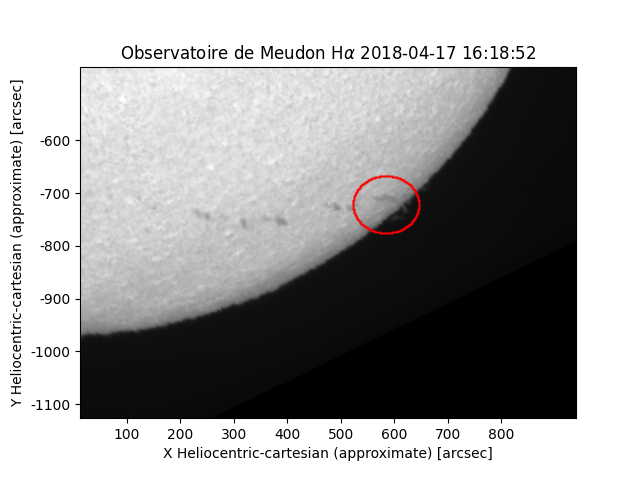
\includegraphics[width=0.8\linewidth]{./01Observations/figs/20180419/ha2.png}
    \caption[The prominence on the days leading up to the IRIS observations.]{The prominence (circled; appearing as a filament) on the days leading up to the IRIS observations. This plot is from \cite{peat_solar_2021}}
    \label{ha}
\end{figure*}
This later manifested as a prominence on the 19 April 2018 off the south western solar limb. This prominence was observed with IRIS, and Hinode \citep{kosugi_hinode_2007} as part of a coordinated observation with the Multichannel Subtractive Double Pass spectrograph \citep[MSDP; ][]{mein_solar_1991} in the Meudon Solar Tower, and the Atacama Large Millimeter/submillimeter Array \citep[ALMA; ][]{wootten_atacama_2009}. The IRIS and Hinode observations start at 14:14 and end at 19:15~UTC. The IRIS observations are made up of a set of 18 very large coarse 32-step rasters using the \ion{C}{ii} (1331.7~\AA-1358.3~\AA), \ion{Si}{iv} (1388~\AA-1406.7~\AA), and \mgii\ (2783.2~\AA-2835.0~\AA) filters along with their complementary slit-jaw imager (SJI) observations, centred on 1330~\AA, 1400~\AA, and 2796~\AA, respectively, with bandpasses of 55~\AA\ in the far-ultraviolet (FUV; \ion{C}{ii} and \ion{Si}{iv}), and 4~\AA\ in the near-ultraviolet (NUV; \mgii) SJI filters. The rasters had a field-of-view (FOV) of 63.9\arcsec$\times$182.3\arcsec\ centred on helioprojective coordinates 632.5\arcsec, $-$753.2\arcsec\ with a clockwise satellite rotation of 51\degr, so that the solar limb was approximately parallel to the y-axis of the instruments. The Hinode observations consisted of X-Ray Telescope \citep[XRT; ][]{golub_x-ray_2007} observations with the Al poly/Open, Open/Gband, and Open/Ti filter combinations with a FOV of 263.3\arcsec$\times$263.3\arcsec, centred on helioprojective coordinates of 607.2\arcsec, $-$749.7\arcsec. The MSDP observations start at 12:05 and end at 16:35~UTC, with a reconstructed FOV of 270\arcsec$\times$370\arcsec\ \citep{barczynski_spectro-imagery_2021}. The ALMA observations were undertaken in Band 3 (2.6-3.6~mm/84-116~GHz) from 15:20 to 17:45~UTC. The FOV of the ALMA observations are of an irregular shape, but are bounded by a box centred on 613.98\arcsec, -771.95\arcsec\ with sides of length 105.00\arcsec$\times$121.80\arcsec. This was the first high resolution interferometric observation of a solar prominence by ALMA \citep[see ][]{labrosse_first_2022}. Whole disc images from the Atmospheric Imaging Assembly \citep[AIA;][]{lemen_atmospheric_2012} onboard the Solar Dynamics Observatory \citep[SDO; ][]{pesnell_solar_2012} were also used. See Fig. \ref{config} for a schematic of this configuration.
  
\begin{figure}
    \centering
    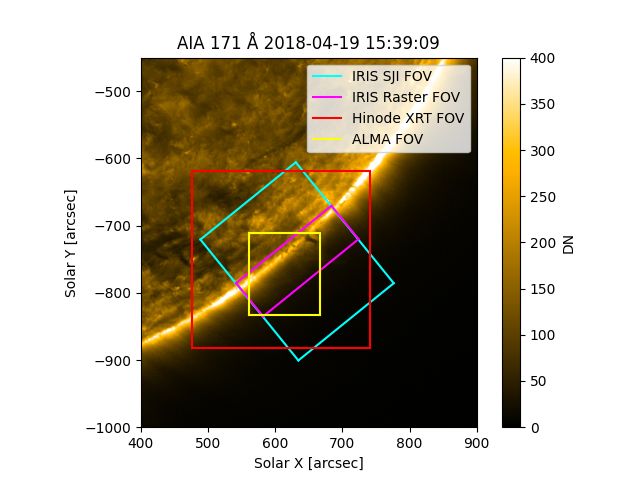
\includegraphics[width=0.93\linewidth]{./01Observations/figs/20180419/Figure_1.png}
    \caption[Configuration of instruments observing the prominence.]{Configuration of instruments observing the prominence. Please note, as the pointing of MSDP is not trivial to determine \citep{barczynski_spectro-imagery_2021}, it is not included in this plot. This plot is from \cite{peat_solar_2021}}
    \label{config}
\end{figure}
 
\begin{figure}
    \centering 
    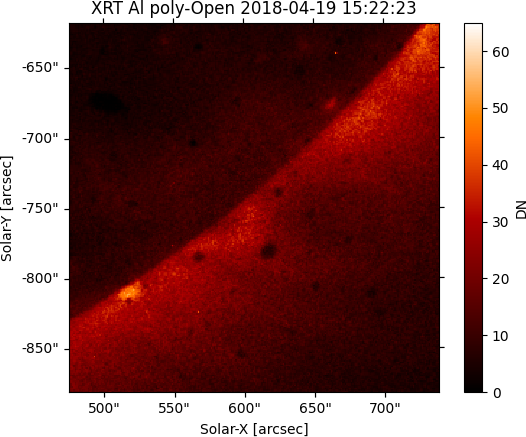
\includegraphics[width=0.6\linewidth]{./01Observations/figs/20180419/xrt.png}
    \caption[Hinode/XRT Al poly/Open observation of the prominence.]{Hinode/XRT Al poly/Open observation of the prominence. The coronal cavity can be clearly seen around (650\arcsec, $-$750\arcsec). This plot is from \cite{peat_solar_2021}}
    \label{xrt}
\end{figure}

The Open/Gband and Open/Ti XRT observations do not show anything of interest over the course of the observation. Al poly/Open also does not show any appreciable change or brightenings over the observation. However, the coronal cavity in which the prominence sits can be seen very clearly seen with this filter (see Fig. \ref{xrt}).

The main focus here is on the IRIS spectra and the information that can be gleaned from it. The IRIS FITS files were retrieved from the Lockheed Martin Solar and Astrophysics Laboratory (LMSAL) website\footnote{https://iris.lmsal.com/} as level 2 fits. Radiometric calibration was performed in Python using the method described in \cite{pereira_itn_2018}, with the appropriate response function retrieved from \texttt{https://hesperia.gsfc.nasa.gov/ssw/iris/response/} as described in \texttt{iris\_get\_response.pro} from SolarSoft \citep[SSW; ][]{freeland_data_1998}. It should be noted that IRIS is calibrated using data from the International Ultraviolet Explorer \citep[IUE;][]{bogges_IUE_1978}, and the spectral radiances recorded by this instrument are given an uncertainty of 10-15\%. As such, this introduces a similar uncertainty to the calibrated IRIS data \citep{tian_itn_2014}. The data was also deconvolved through Python following similar operations to that of \texttt{iris\_sg\_deconvolve.pro} from SSW\footnote{A full Python implementation of these procedures can be found at https://github.com/OfAaron3/irispreppy, or by simply running pip install irispreppy.}. The AIA files were retrieved from the Virtual Solar Observatory (VSO) as level 1 FITS. These were then prepared to level 1.5 through \texttt{aia\_prep.pro} from SSW in IDL. The 304~\AA\ filter shows similar behaviour to that seen in the \mgii~k SJI from IRIS. This is expected as both channels have high chromospheric to low transition region origins \citep{lemen_atmospheric_2012, depontieu_interface_2014}. 

The \mgii~k/2796~\AA\ SJI images show a very dynamic prominence with many flows, the bulk of which propagates towards the south-western limb \figp{threestages}. The observations culminate with a large flow extending down from the top of the prominence towards the southern solar limb.

The 171~\AA\ filter shows a small barb seen in absorption; this is where the prominence is anchored to the solar surface. This corresponds to the densest and most central part of the prominence. We expect to see strong central reversals in the area of the prominence due to the higher density in this location. In 171~\AA, we also see a faint shroud surrounding the barb, with its shape very similar to what is seen in 304~\AA. and \mgii~k. This can be interpreted as the prominence-to-corona transition region (PCTR) as the 171~\AA\ filter is senstive to spectral lines formed at transition region (TR) and coronal temperatures.

\begin{figure}
    \centering
    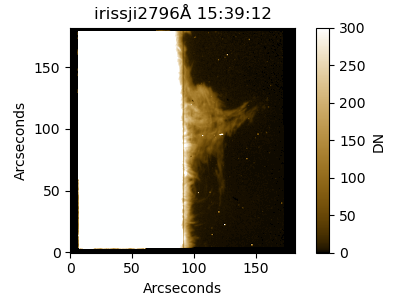
\includegraphics[width=0.32\linewidth]{./01Observations/figs/20180419/MgIISJI0.png}
    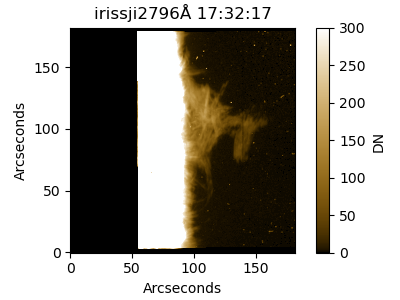
\includegraphics[width=0.32\linewidth]{./01Observations/figs/20180419/MgIISJI1.png}
    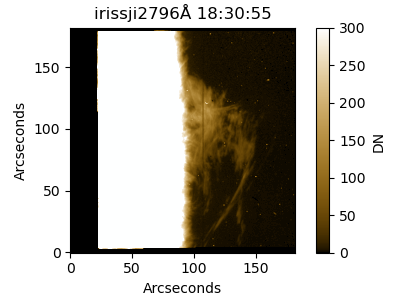
\includegraphics[width=0.32\linewidth]{./01Observations/figs/20180419/MgIISJI2.png}
    
    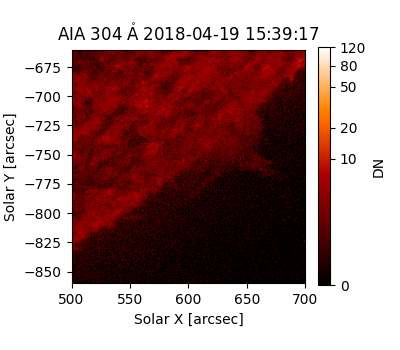
\includegraphics[width=0.32\linewidth]{./01Observations/figs/20180419/304_0.png}
    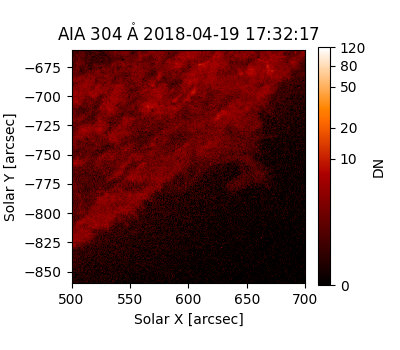
\includegraphics[width=0.32\linewidth]{./01Observations/figs/20180419/304_1.png}
    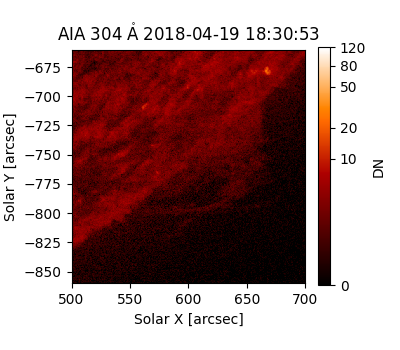
\includegraphics[width=0.32\linewidth]{./01Observations/figs/20180419/304_2.png}

    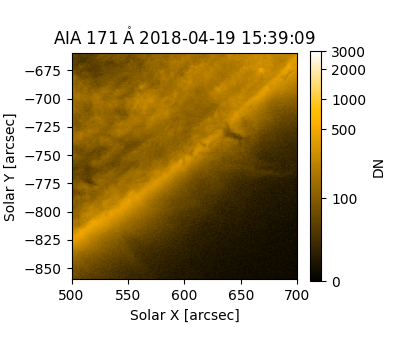
\includegraphics[width=0.32\linewidth]{./01Observations/figs/20180419/171_0.png}
    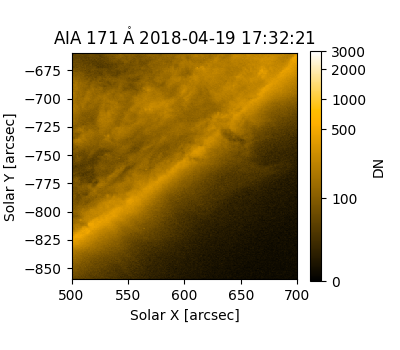
\includegraphics[width=0.32\linewidth]{./01Observations/figs/20180419/171_1.png}
    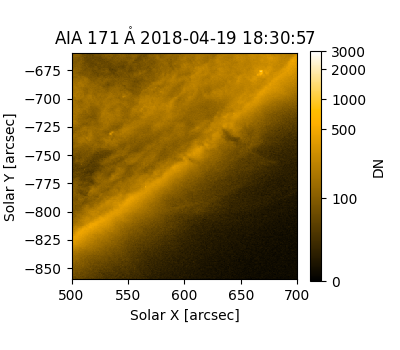
\includegraphics[width=0.32\linewidth]{./01Observations/figs/20180419/171_2.png}
    
    \caption[The key three stages of the development of the prominence.]{Observations of the prominence during the key three stages of its development. The top, middle, and bottom rows show the IRIS SJI \mgii~k, SDO/AIA 304\AA, and SDO/AIA 171\AA\ filters, respectively. \textit{Left} shows small flows towards the limb. \textit{Middle} shows the beginning of the large flow, where plasma extends out of the top of the prominence. \textit{Bottom} Shows the large flow towards the limb. These plots are from \cite{peat_solar_2021}.}
    \label{threestages}
\end{figure}

After the end of the IRIS, Hinode, MSDP, and ALMA observations, the prominence persists in 171~\AA{} and 304~\AA. In 304~\AA, the prominence continues to exhibit dynamic behaviour and appears to fall towards the limb over the next 24 hours. This is a consequence of the projection effect, as it rotates out of view. This behaviour is not mirrored in 171~\AA. The barb and shroud instead appear to fade away as they become occulted by brighter coronal emission. On 22 April, the structure appears again in the 171~\AA{} and 304~\AA{} filters of EUVI, part of the Sun Earth Connection Coronal and Heliospheric Investigation \citep[SECCHI; ][]{howard_sun_2008} on board the Solar Terrestrial Relations Observatory (Ahead) \citep[See Fig \ref{secchi}; STEREO-A; ][]{driesman_stereo_2008}. The prominence is observed to continue to transit across the disc and no filament eruption is observed. At this time, STEREO-A was approximately 117\degr{} west of the Earth.

\begin{figure}
    \centering
    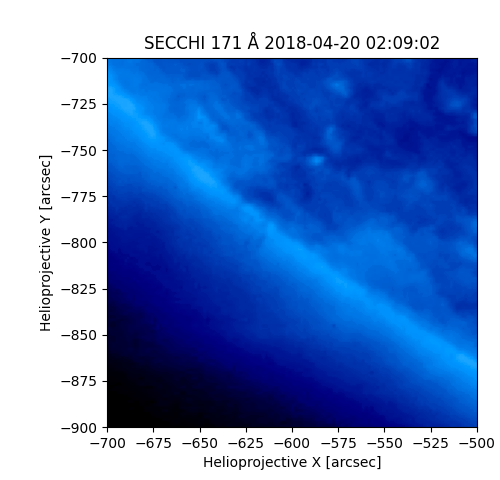
\includegraphics[width=0.49\linewidth]{./01Observations/figs/20180419/secchi171.png}
    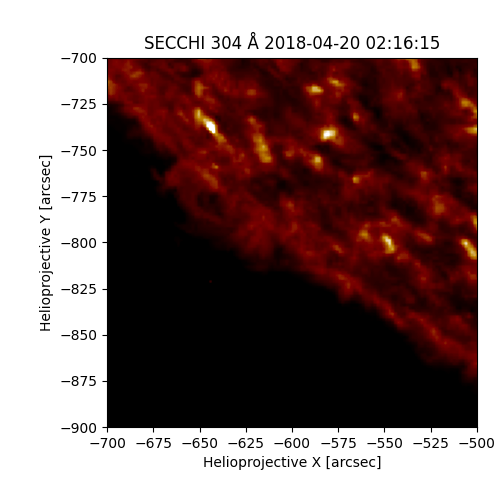
\includegraphics[width=0.49\linewidth]{./01Observations/figs/20180419/secchi304.png}
    \caption[The prominence as it appears on the 20 April 2018 in EUVI on SECCHI.]{The prominence as it appears on the 20 April 2018 in EUVI on SECCHI. \textit{Left}: The prominence barb reappearing in 171~\AA. \textit{Right}: The prominence structure in 304~\AA.}
    \label{secchi}
\end{figure}

\begin{figure}
    \centering
    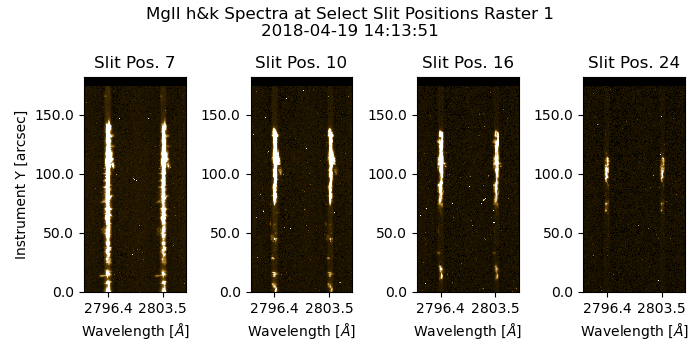
\includegraphics[width=.85\linewidth]{./01Observations/figs/20180419/slit1.png}
    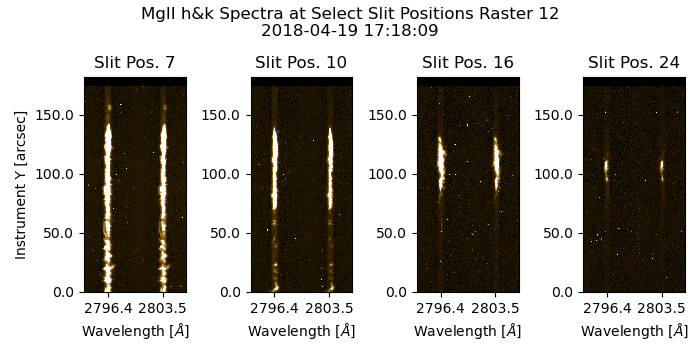
\includegraphics[width=.85\linewidth]{./01Observations/figs/20180419/slit12.png}
    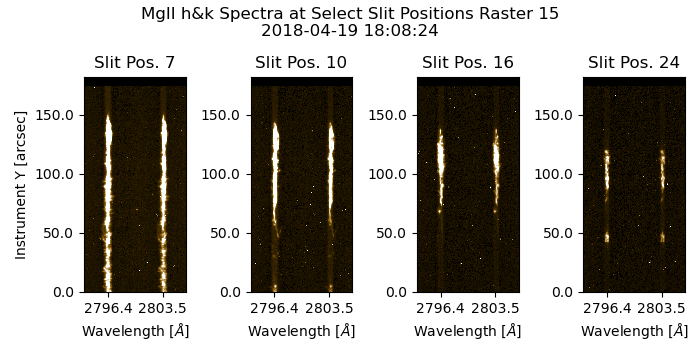
\includegraphics[width=.85\linewidth]{./01Observations/figs/20180419/slit15.png}
    \caption[\mgiihk\ at select slit positions and rasters. See Fig. \ref{fig:hmaps} and Fig. \ref{fig:kmaps} for context.]{\mgiihk\ at select slit positions and rasters. See Fig. \ref{fig:hmaps} and Fig. \ref{fig:kmaps} for these slit position in context. There is a wide range of profile shapes present, and a few where several structures are clearly present. These plots are from \cite{peat_solar_2021}.}
    \label{spectra}
\end{figure}

\begin{figure}
    \centering
    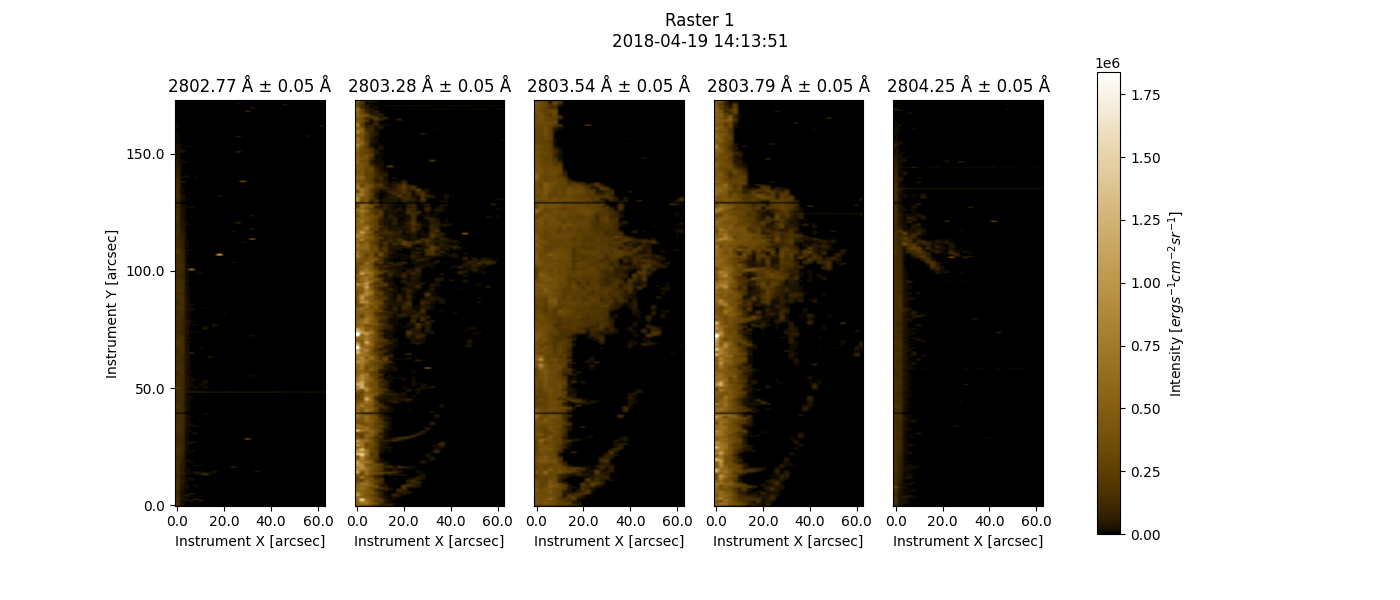
\includegraphics[width=0.9\linewidth]{01Observations/figs/20180419/spectrogramh1.png}
    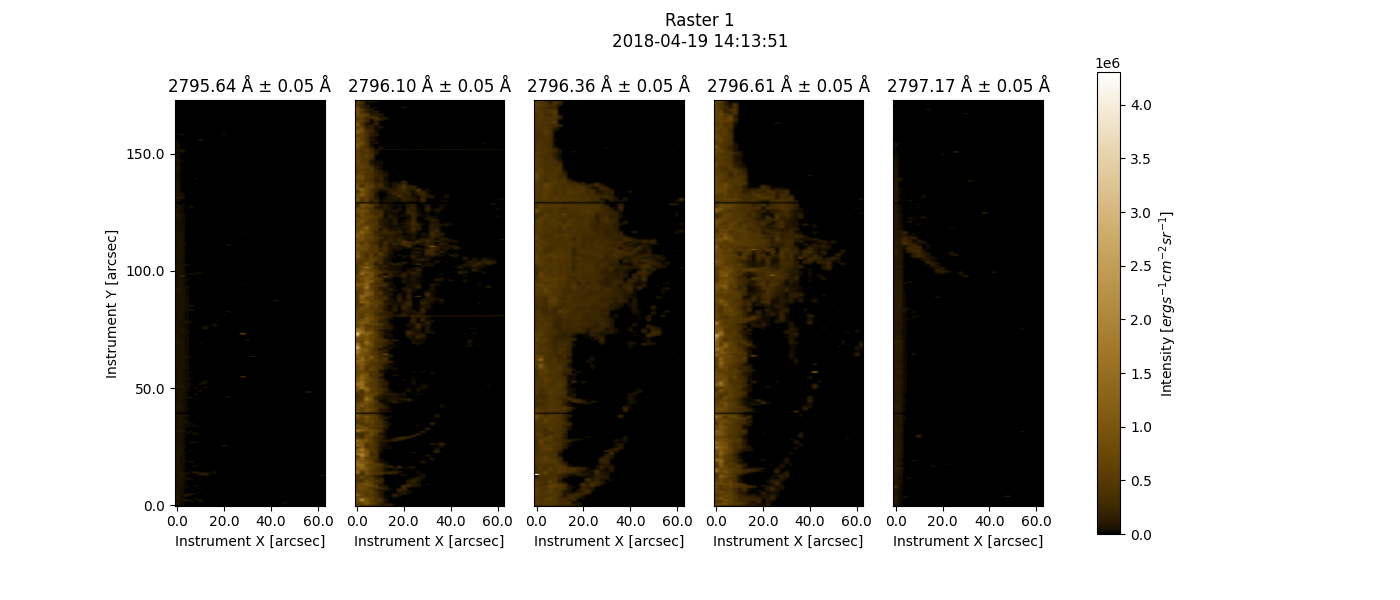
\includegraphics[width=0.9\linewidth]{01Observations/figs/20180419/spectrogramk1.png}
    \caption[\mgiihk{} maps at different points along the wavelength window. In the rightmost/redshift panel, an isolated structure is observed.]{\mgiihk\ (top and bottom respectively) maps at different points along the wavelength window. In the rightmost/redshifted panel, an isolated structure is observed.}
    \label{fig:extraboi}
    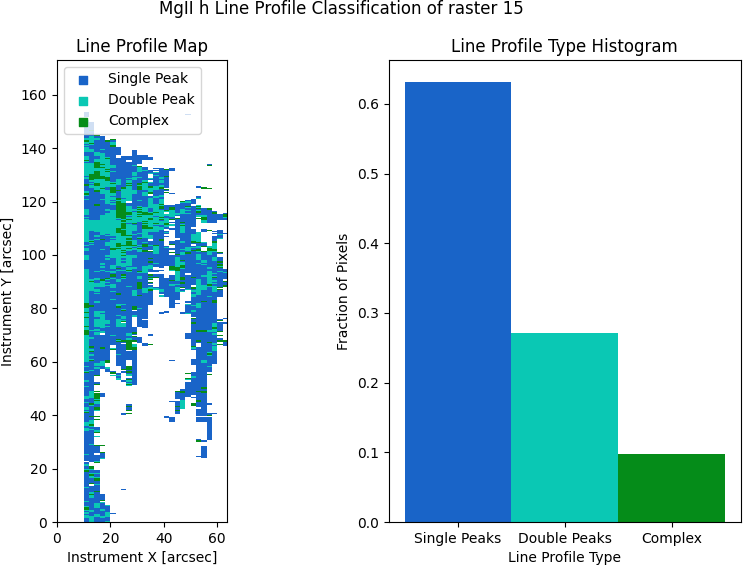
\includegraphics[width=.47\linewidth]{./01Observations/figs/20180419/h14lt.png}
    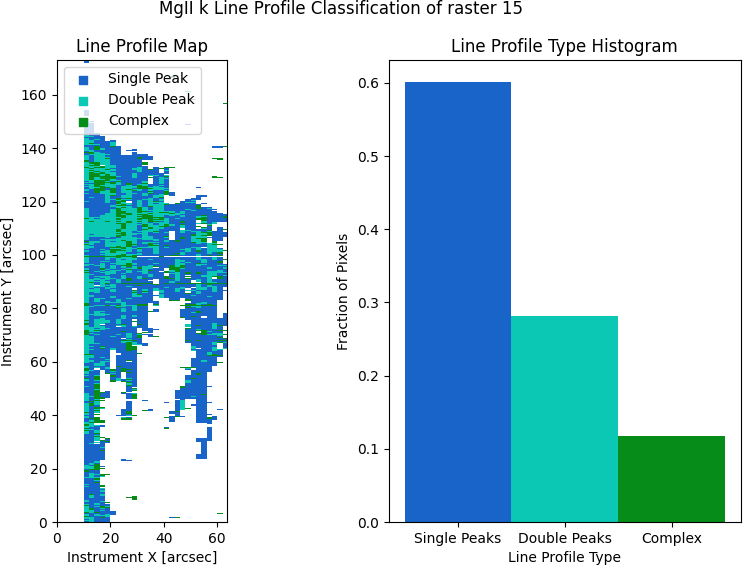
\includegraphics[width=.47\linewidth]{./01Observations/figs/20180419/k14lt.png}
    \caption[Distribution of line types seen in \mgiihk\ in raster 14.]{Distribution of line types seen in \mgiihk\ in raster 14. A complex line profile is any line profile found to have two or more than three turning points. The left plot is from \cite{peat_solar_2021}}
    \label{linetypes}
\end{figure}

\begin{figure} 
    \centering
    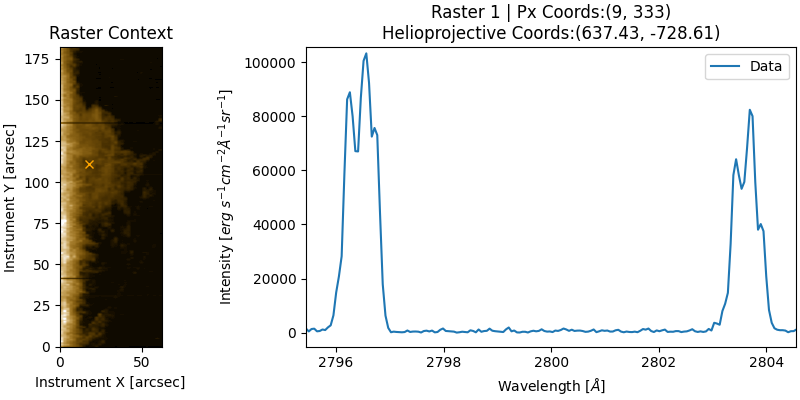
\includegraphics[width=0.8\linewidth]{./01Observations/figs/complex.png}
    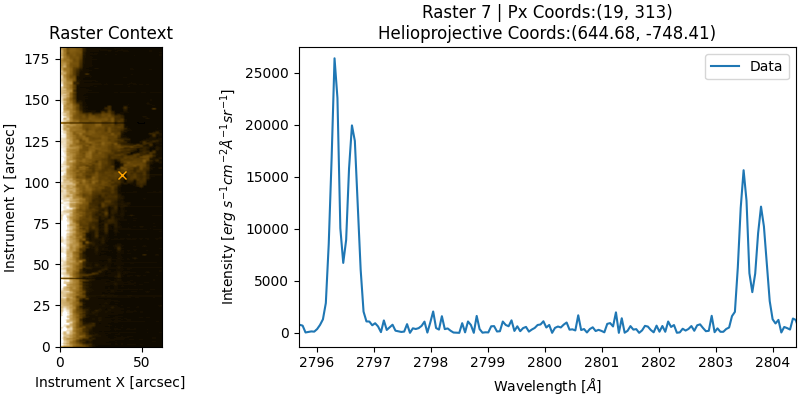
\includegraphics[width=0.8\linewidth]{./01Observations/figs/double.png}
    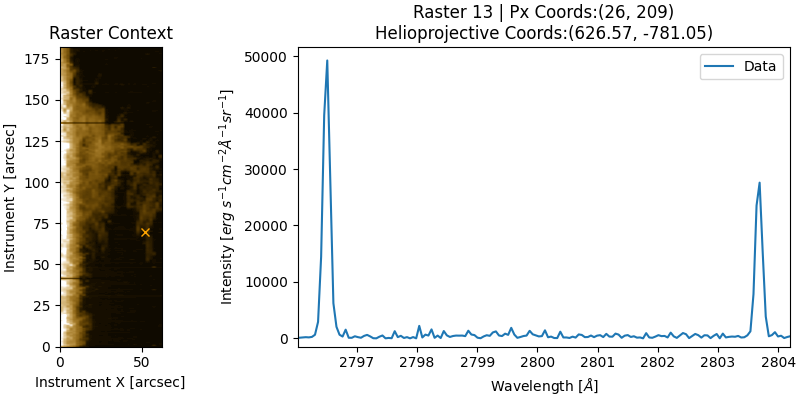
\includegraphics[width=0.8\linewidth]{./01Observations/figs/single.png}
    \caption{Examples of the three different classifications of peaks. \textit{Top}: Complex. \textit{Centre}: Double peaked. \textit{Bottom}: Single peaked.}
    \label{threespectratypes}
\end{figure}

The \mgii~h\&k spectra from the core of the prominence display many complex structures. This carries the implication that there are many structures along the line of sight. One notable example of this can be seen in the top panel of Fig. \ref{spectra} at approximately 110\arcsec\ in slit position 7. Here there are clearly two different peaks, one near the rest wavelength, and a second highly redshifted. This can be seen more clearly in \fig{fig:extraboi}. The structure producing these highly redshifted peaks is very easily seen through the wings of the at-rest \mgii\ in front of it. This structure is likely behind the prominence as it disappears in the subsequent rasters. This occurrence is not unique to this case, and is quite common throughout the prominence. This is, however, the most extreme example. As one may expect, the prominence  spectra are composed of many different types of line profiles. This distribution can be seen in Fig. \ref{linetypes}. To find the distribution of line profile types, the numerator of the difference quotient was solved for each pixel in a 3~\AA{} window centred on \mgiihk{}, respectively,
\begin{equation}
    \frac{df(\lambda)}{d\lambda}=\frac{f(\lambda+\Delta\lambda)-f(\lambda)}{\Delta\lambda}.
\end{equation}
If the numerator changed polarity between two successive pixels, this was counted as a turning point. If one turning point was found, that pixel would be classed as having a single peak; if three were found, it would be classed as a reversed profile; if any other number was found, it would be classed as complex. The classification of any line profile with two peaks is ambiguous, and so is classed as complex (see \fig{threespectratypes} for an example of these). To avoid counting turning points in the noise, an intensity threshold was set, where any turning point below that intensity threshold was discarded.While single peak profiles dominate the distribution, double peaked and complex profiles are not negligible, with roughly 10\% to 20\% of the profiles appearing complex in both h and k. The large branch observed to be extending towards the limb near the end of the observation appears to exhibit mostly single peaked profiles along with some double peaks. Additionally, it appears to have some profiles classed as single peaks that are in fact double peaks suffering from an effect further discussed in Sect. \ref{velsect}, where the emission of h$_{2r}$ and k$_{2r}$ is lower than that of h$_{3}$ and k$_{3}$, therefore no turning point is produced here. This results in only the h$_{2v}$ and k$_{2v}$ peaks being pronounced enough such that $\dd I/\dd \lambda=0$ at these peaks. This effect is also present in the reverse scenario. This can be interpreted in one of two ways - the line profile is double peaked, but is so Doppler shifted that one of the peaks ends up in the rest line core and is absorbed; or there exists more than one thread of plasma at different line-of-sight velocities leading to a false double peak. In the former case, the plasma would require high density, temperature or large geometrical thickness to produce a double peak, and then it would require a large line-of-sight velocity to produce this effect. The latter, however, has less extreme prerequisites. Additionally, prominences are known to be comprised of many threads moving at a plethora of line-of-sight velocities \citep{engvold_fine_1978}, and so we interpret this as such \seef{k2vgtk2r}.

\begin{figure} 
    \centering
    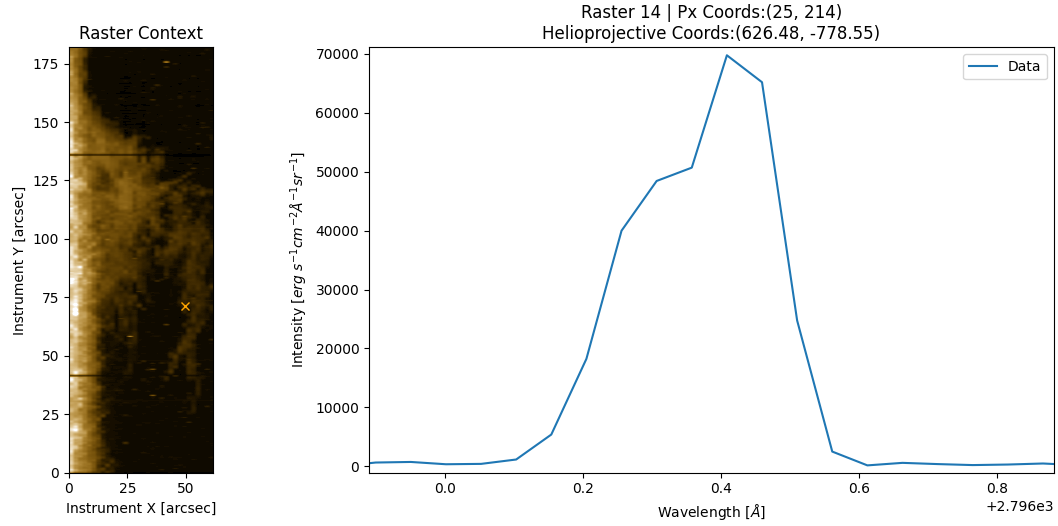
\includegraphics[width=0.7\linewidth]{./01Observations/figs/asym.png}
    \caption{Asymmetry in \mgii~k where it could be argued that there are two peaks due to there likely being two threads along the line of sight. However, this profile was classified as having a single peak.}
    \label{k2vgtk2r}
\end{figure}






% \begin{figure}
%     \centering

% \end{figure}
Here, we focus mainly on the NUV filter of IRIS. The prominence appears only very faintly in the FUV bands, making analysis difficult. Additionally, increasing the contrast in the FUV bands enough to see the prominence leads to the appearance of a ghost image of the aperture of the telescope on the image. This is due to parasitic light and only affects FUV off-limb observations, the NUV channels are unaffected by this \citep{wulser_instrument_2018}.
\section{The Quantile Method}
\label{quantile_method}
\begin{figure}
    \centering
    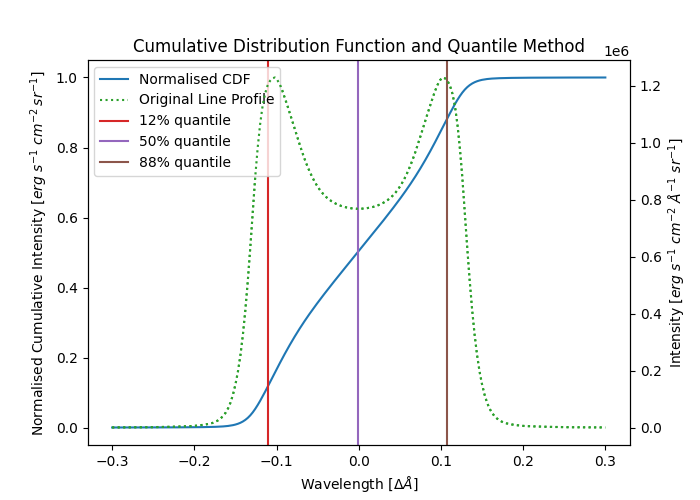
\includegraphics[width=.9\linewidth]{./01Observations/figs/20180419/cdf.png}
    \caption{Cumulative Distribution Function of a synthetic line profile as an example; with its associated 12\%, 50\%, and 88\% quantiles.}
    \label{cdfex}
\end{figure}

We use the quantile method \citep{kerr_iris_2015,ruan_dynamic_2018} to determine the FWHM, line core shift, and asymmetry of the line profiles to explore the dynamics and structure of the prominence. The quantile method involves calculating the cumulative distribution function (CDF) over the intensity of the line profiles over some wavelength range. We use two 3~\AA\ windows centred on the rest wavelengths of \mgiihk. We then linearly interpolate over these CDFs to find the wavelengths corresponding to the 12\%, 50\%, and 88\% levels of the CDFs ($\lambda_{12}, \lambda_{50}, \lambda_{88}$). $\lambda_{50}$ is defined as the line core and is used to find the line core shift in km~s$^{-1}$. To obtain a value for $\lambda_\text{rest}$, we applied the quantile method on the first slit of the raster. This first slit is on the solar disc, and we employ a 3\AA{} window centred on the rest vaccuum wavelengths of \mgiihk{}, respectively, to obtain a value for the rest wavelengths of both h and k. The mean of these rest wavelengths, in h and k, was then taken and used as $\lambda_\text{rest}$ in \eq{eq:vdop}. Assuming that the lines are Gaussian in nature, the FWHM can be determined by finding the difference between $\lambda_{88}$ and $\lambda_{12}$. However, not all of our profiles are Gaussian, and we instead use this as a measurement of line width. All three of these values are used to determine the asymmetry. As equations, they are as follows,

\begin{equation}
    v_\text{dop}=\left(\frac{\lambda_{50}}{\lambda_{\text{rest}}}-1\right)c,
    \label{eq:vdop}
\end{equation}
\begin{equation}
    \text{Line Width}=~\lambda_{88}-\lambda_{12},
    \label{eq:fwhm}
\end{equation}
\begin{equation}
    \text{Asymmetry}=~\frac{\left(\lambda_{88}-\lambda_{50}\right)-\left(\lambda_{50}-\lambda_{12}\right)}{\lambda_{88}-\lambda_{12}},
    \label{eq:asym}
\end{equation}
%overfull hbox craziness be here. This comment fixes it.
where $\lambda_{\text{rest}}$ is the rest wavelength of the line, and $c$ is the speed of light. A graphical representation of these quantiles can be seen in Fig. \ref{cdfex}. The maps resulting from these equations can be seen in Figs. \ref{fig:hmaps} and \ref{fig:kmaps} for h\&k, respectively.
 
Coronal pixels were removed from the \mgii~h\&k rasters using the quantile method. From line width maps, chromospheric-like structures, such as the prominence and spicules, are very clearly separated from the solar disc and coronal pixels \sectp{lwid}. Therefore, by calculating the line width of every pixel for every raster via the quantile method coronal pixels could be removed. Coronal pixels will be found to exhibit large line widths compared to data and will be clearly separated in a histogram. This is not a true measure of line width, as in coronal pixels there is no \mgiihk{} emission to measure here, but the method still returns a value. This produces a double peaked distribution in the line width histogram. The minimum turning point of this distribution is selected as the cut off value, where values higher than this are considered to be coronal pixels \figp{lwHist}. However, some non-coronal pixels truly do have a large line width. To combat these false positives, the pixels are then subject to a simple intensity filter. Any of these would-be discarded pixels that are above the threshold are relabelled as not coronal. This limit was set as twice the mean intensity of every pixel of every raster in two 3~\AA\ wide windows centred on the rest wavelengths of \mgiihk, respectively.  The result of this filtering can be seen in Fig. \ref{filtresult}. Since the publication of \cite{peat_solar_2021}, the work on which this section is based, this filter now includes an extra step to remove any rogue coronal pixels that slip through the filter. Inspired by the death by underpopulation rule from John Conway's Game of Life \citep{martin_mathematical_1970}, any unremoved pixel that has 2 or fewer unremoved 2-connected neighbours (the surrounding pixels) is also removed. 

In order to estimate the error associated with the Doppler velocity, line width and asymmetry, a synthetic double peaked line profile was used from PROM \sectp{promintro}. This profile was downscaled to the same resolution as the IRIS spectrograph and padded with zeros such that it was 3~\AA{} wide. Then, using the filtered rasters, the every pixel's mean value between 2797.85~\AA{} and 2802.03~\AA{} was taken. The standard deviation and mean of these values were taken in order to estimate Gaussian noise. This noise was randomly added to the synthetic line profile and the Doppler velocity, line width, and asymmetry were calculated using the quantile method for \mgiihk, respectively. This was repeated one million times to acquire a large sample size. A Gaussian was then fitted to the histograms of these distributions in order to recover a standard deviation which we will quote as the error of these measurements. For \mgii~h, the standard deviations were found to be $0.369$~\kms, $3.94\times10^{-3}$~\AA, and $2.00\times10^{-2}$~\AA{} for Doppler velocity, line width, and asymmetry, respectively. For \mgii~k, the standard deviations were found to be $0.225$~\kms, $2.03\times10^{-3}$~\AA, and $1.58\times10^{-2}$~\AA{} for Doppler velocity, line width, and asymmetry, respectively.

\begin{figure}
    \centering
    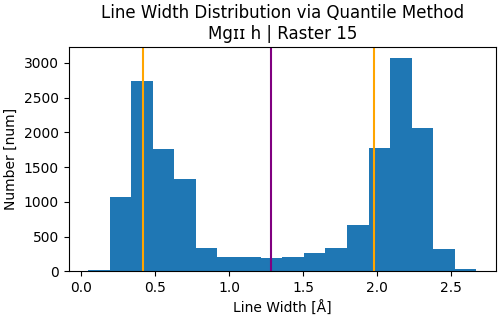
\includegraphics[width=0.49\linewidth]{./01Observations/figs/h15.png}
    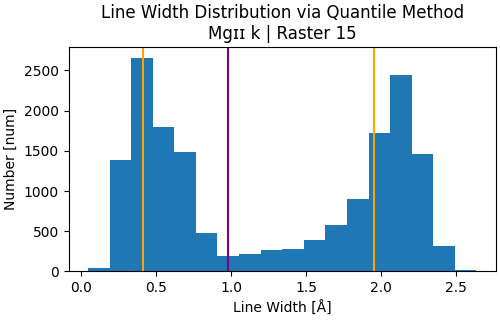
\includegraphics[width=0.49\linewidth]{./01Observations/figs/k15.png}
    \caption[Histogram of the line widths of \mgiihk{} in raster 15.]{Histogram of the line widths of \mgiihk{} in raster 15. The purple vertical line indicates the local minimum and cut off point and the orange lines represent the range over which the minimum turning point is searched for.}
    \label{lwHist}
\end{figure}

\begin{figure}
    \centering
    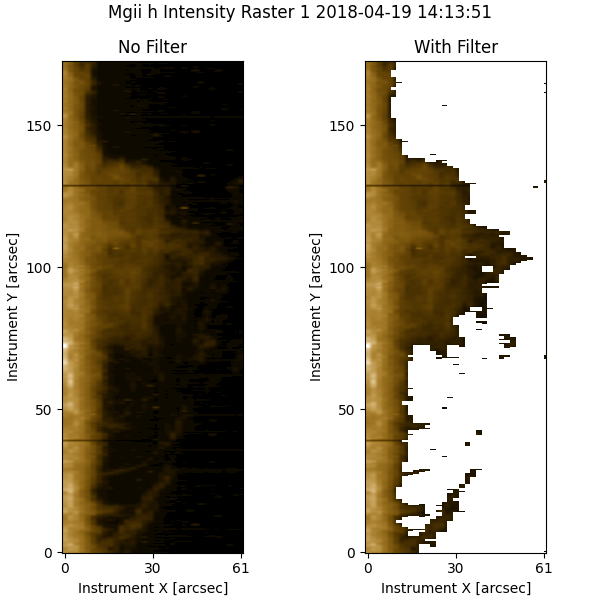
\includegraphics[width=0.6\linewidth]{./01Observations/figs/20180419/Figure_2.png}
    \caption[Example of a resulting \mgii~h map with the filtering applied.]{Example of a resulting \mgii~h map with the filtering applied. \textit{Left}: \mgii~h without the filter and \textit{Right}: \mgii~h with the filter. This plot is from \cite{peat_solar_2021}}
    \label{filtresult}
\end{figure}



\begin{figure}
    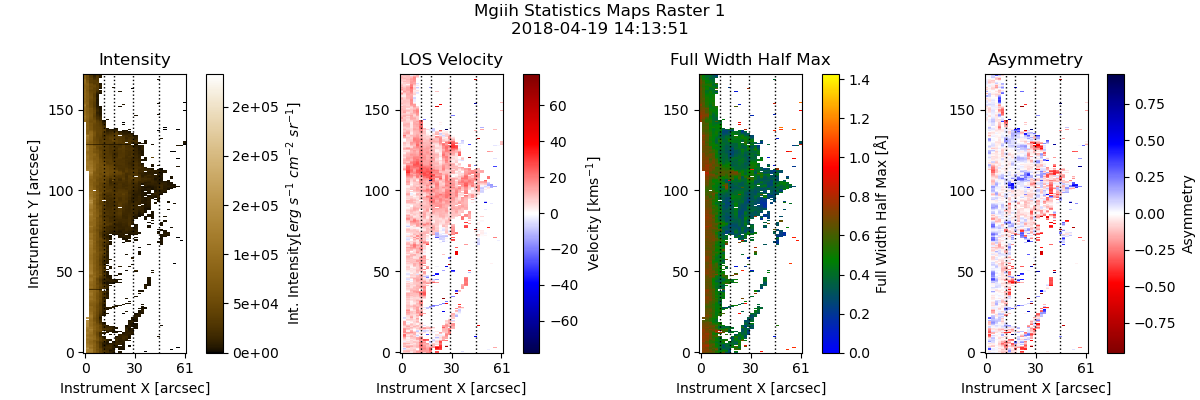
\includegraphics[width=\linewidth]{./01Observations/figs/20180419/hmaps0.png}
    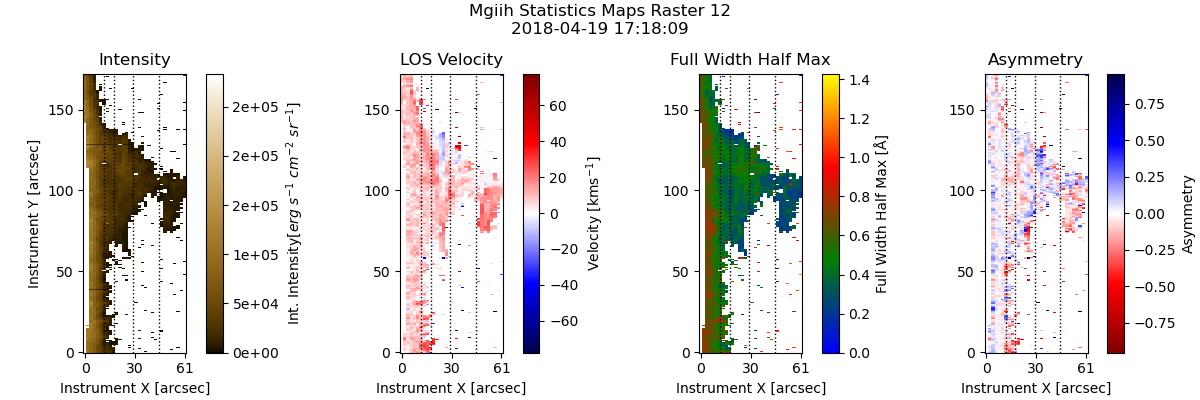
\includegraphics[width=\linewidth]{./01Observations/figs/20180419/hmaps1.png}
    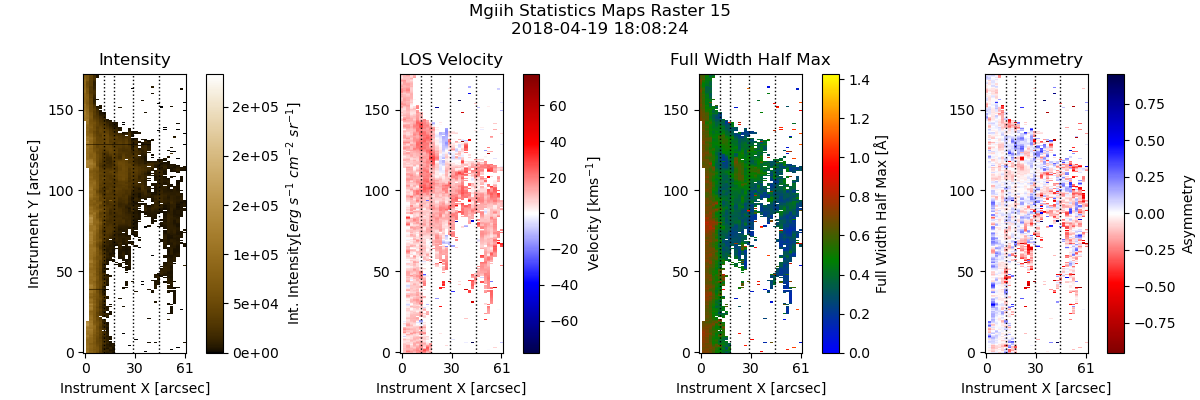
\includegraphics[width=\linewidth]{./01Observations/figs/20180419/hmaps2.png}
    \caption[\mgii~h statistics maps of the three main stages of the prominence.]{\mgii~h statistics maps of the three main stages of the prominence observation calculated via equations \ref{eq:vdop}, \ref{eq:fwhm}, and \ref{eq:asym}. The times associated with these plots are the time at the beginning of the associated raster scan. The four dotted lines correspond to the spectra presented in Fig. \ref{spectra}. These plots are from \cite{peat_solar_2021}.}
    \label{fig:hmaps}
\end{figure}

\begin{figure}
    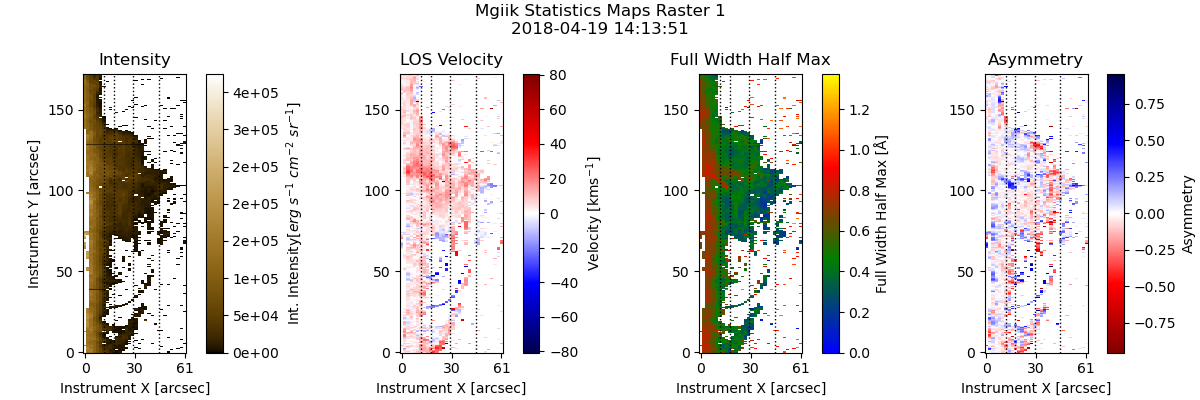
\includegraphics[width=\linewidth]{./01Observations/figs/20180419/kmaps0.png}
    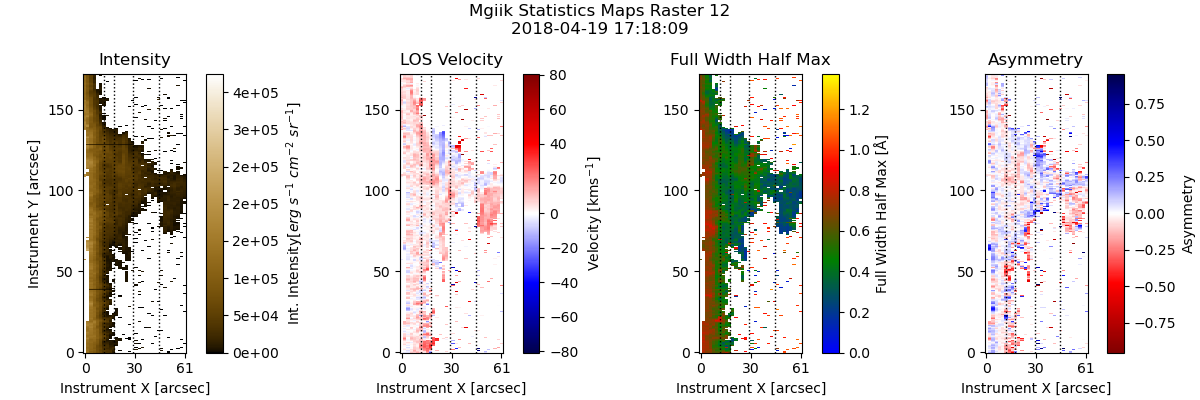
\includegraphics[width=\linewidth]{./01Observations/figs/20180419/kmaps1.png}
    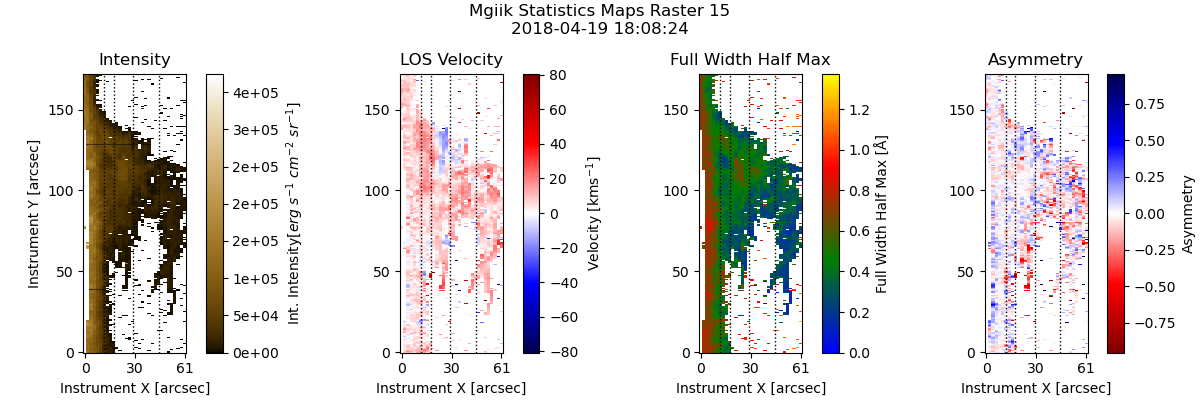
\includegraphics[width=\linewidth]{./01Observations/figs/20180419/kmaps2.png}
    \caption[\mgii~k statistics maps of the three main stages of the prominence.]{Same as \fig{fig:hmaps} for \mgii{}k. This plot is from \cite{peat_solar_2021}.}
    \label{fig:kmaps}
\end{figure}

\section{Line Core Shift and Asymmetry}
\label{velsect}

The prominence displays a wide range of line core shift ranging from $-$74 to 78~km~s$^{-1}$ and $-$72 to 85~km~s$^{-1}$ in \mgiihk, respectively. Both display Gaussian-like distributions centred on a mean redshift of 8.20~km~s$^{-1}$ and 5.2~km~s$^{-1}$ with standard deviations of 5.98~km~s$^{-1}$ and 6.61~km~s$^{-1}$, respectively. The extreme velocities found here are very rare, and this is reflected in \fig{fig:velgauss} where most material is found to be moving in the range -20\kms{} to 30\kms.  
\begin{figure}
    \centering
    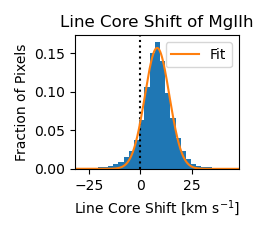
\includegraphics[width=0.35\linewidth]{./02Modelling1D/figs/20180419/hvelocities.png}
    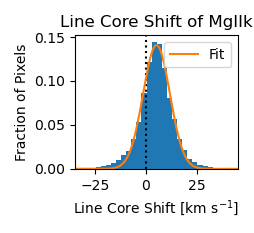
\includegraphics[width=0.35\linewidth]{./02Modelling1D/figs/20180419/kvelocities.png}
    \caption[Distribution of line core shifts found in the prominence.]{Distribution of line core shifts found in the prominence. \textit{Left}: \mgii~h. \textit{Right}: \mgii~k. These plots are from \cite{peat_solar_2021}.}
    \label{fig:velgauss}
\end{figure}
These velocities are consistent with those seen in past observations. \cite{liggett_rotation_1984} observed velocities ranging from 12 to 75~km~s$^{-1}$; \cite{schmieder_reconstruction_2017} found maximum velocities of around 60~km~s$^{-1}$; and Table 6 from the review by \cite{labrosse_physics_2010} shows a range of velocities exhibited by EUV prominences with an extreme of 70~km~s$^{-1}$, centred around 20\kms. The Gaussian fits used to model the distributions of line core shifts does not seem to match well at the wings. This may be due to ``asymmetry bias'', where line profiles with large asymmetry are mistakenly measured to have a large Doppler velocity via the quantile method. This is due to the increased influence of h$_{2\text{v}}$/k$_{2\text{v}}$ for those of high blueshift, or h$_{2\text{r}}$/k$_{2\text{r}}$ for those with high redshift, as these peaks move into the more optically thin regime in the wings, increasing their peak intensity. This effect is further exaggerated by the opposite effect, where the h$_{2\text{r}}$/k$_{2\text{r}}$ for high blueshift, or the h$_{2\text{v}}$/k$_{2\text{v}}$ for high redshift, move into the more optically thick regime in the core, decreasing their peak intensity. This is not something that can be simply corrected for if we wish to continue using the quantile method. This effect is illustrated in Fig. \ref{fig:hda}. It is then therefore suggested that the line core shift found by the quantile method in areas of high asymmetry are not to be trusted. Line core shifts of pixels are therefore more reliable the closer to zero their respective asymmetry. Line core shift and asymmetry are very strongly linked. Line profile asymmetry is strongest in the branch extending down from the main body near to the end of the rasters. The asymmetries of these line profiles are in the range [0, -1), suggesting, as discussed in Sect. \ref{velsect}, that many of these may be highly redshifted. This is true, but the branch is mainly comprised of single profiles which are not so sensitive to this effect. Instead we observe a mix of asymmetrical line profiles, and low intensity and low width lines \figp{asyms}. Our wide 3~\AA\ window causes the quantile method to measure overestimate the asymmetry of the latter. This could be another explanation for the relationship seen in \fig{fig:hda}. Asymmetry and line core shift appear to be anticorrelated as shown in \fig{fig:hda}, however, the structure around 110~\arcsec in raster 1 appears to break this trend. Therefore, the asymmetry and line width, calculated via the quantile method, together would perhaps be a better proxy for whether a pixel contains more than one profile, rather than line width alone. This may be the reason that we observe an overall redshift from even though we have corrected for solar rotation. 

It is difficult to quantify the uncertainty that the asymmetry causes on the measurement of line core shift. This is because you are required to know the `true' line core shift. This is not easily determined due to the multithreaded nature we see in line profiles from solar prominences. By that rationale, one could argue that the measurements of line core shift themselves are not entirely reliable either. This brings us back to the same conclusion from earlier where we suggest that line core shifts of pixels are more reliable the closer to zero their respective asymmetry.

\begin{figure}
    \centering
    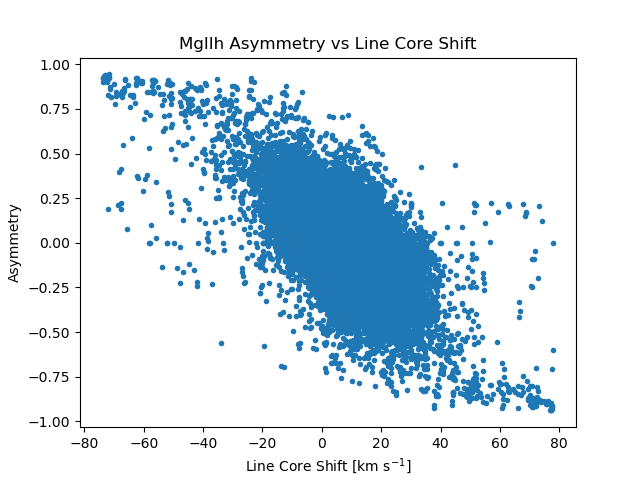
\includegraphics[width=0.7994\linewidth]{01Observations/figs/20180419/hda.png}
    \caption[Asymmetry against line core shift for all prominence pixels in every raster.]{Asymmetry against line core shift for all prominence pixels in every raster. This demonstrates the effect of ``asymmetry bias'' when measuring line core shift with the quantile method. This plot is from \cite{peat_solar_2021}}
    \label{fig:hda}
\end{figure}

\section{Line Widths}
\label{lwid}
As mentioned in Sect. \ref{quantile_method}, line width is measured by \eq{eq:fwhm}. The line width maps clearly separate the chromospheric-like structures, such as the prominence and spicules, from the solar disc, with the disc displaying line widths of greater than approximately 0.8~\AA\ and the spicules and the prominence displaying much less. As discussed in Sect. \ref{20180419main}, it also clearly distinguishes the coronal pixels from the prominence. This of course, is not shown on the Fig. \ref{fig:hmaps} and Fig. \ref{fig:kmaps} as it is filtered out. The large measured line width is just a consequence of using the quantile method to measure the line widths. There are no \mgiihk\ line profiles in the corona to measure the width of, but a CDF is still created and analysed as if there were \mgiihk{} emission. In non-filtered diagnostic maps, line width is a good way to view the bulk motion of low intensity features difficult to distinguish in intensity maps \figp{fwhmex}.

\begin{figure}
    \centering
    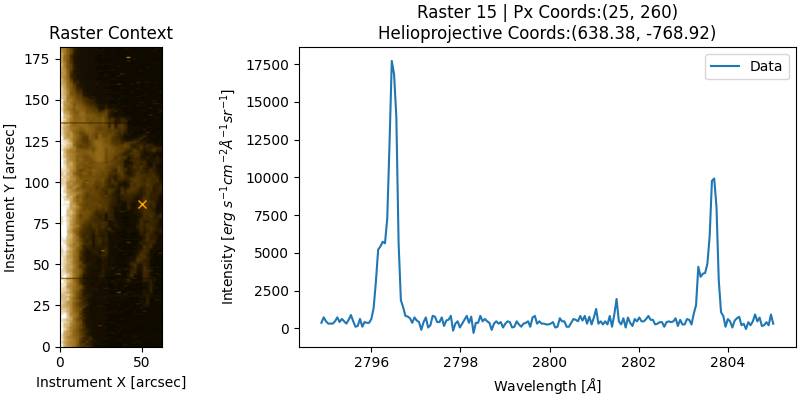
\includegraphics[width=0.6\linewidth]{./01Observations/figs/20180419/asym1.png} 
    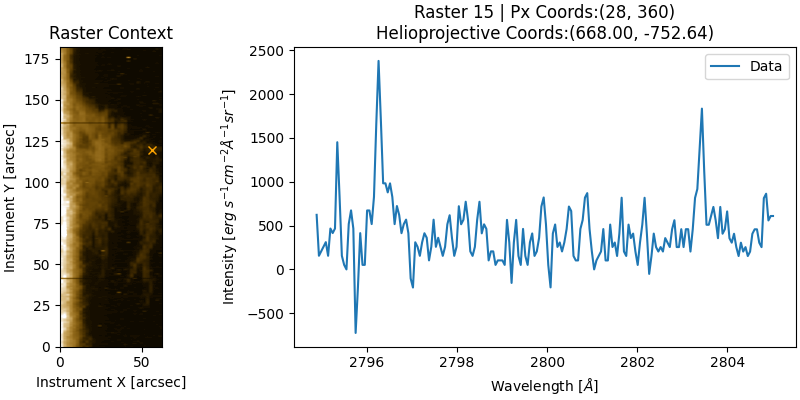
\includegraphics[width=0.6\linewidth]{./01Observations/figs/20180419/asym4.png}
    \caption[Two examples of the types of \mgiihk{} line profiles seen in the branch]{Two examples of the types of \mgiihk{} line profiles seen in the branch. \textit{Top}: Asymmetric line profiles. \textit{Bottom}: Low intensity and line width lines.}
    \label{asyms}
\end{figure}


In the first raster (14:13:51~UTC), we see a structure of large line width around 110\arcsec\ in y. This is due to the presence of at least two structures along the line of sight, with one highly redshifted profile. This can be seen in Fig. \ref{fig:extraboi}, where this structure is most easily seen. This structure is only visible in the first raster. 

The location of this appears to correlate with the location of the barb seen in the 171~\AA\ AIA filter \seef{threestages}. However, the barb does not disappear after the first raster, as this is where the prominence is anchored to the solar surface. However, this does correlate with the highest density area of the prominence and so this behaviour, while extreme, is to be expected. This demonstrates one of the drawbacks of the quantile method, it cannot distinguish between line profiles. It simply includes both profiles in the calculation and produces a number for line width, albeit a large one. This could perhaps be used as a proxy for a pixel containing more than one line profile, but this is outside the scope of this study. Alternatively, an attempt to fit several Gaussian profiles to this location could be attempted. However, this is a highly degenerate problem, and even if it were not, it would be slow. One of the main advantages of the quantile method is its expediency. 


\begin{figure}
    \centering
    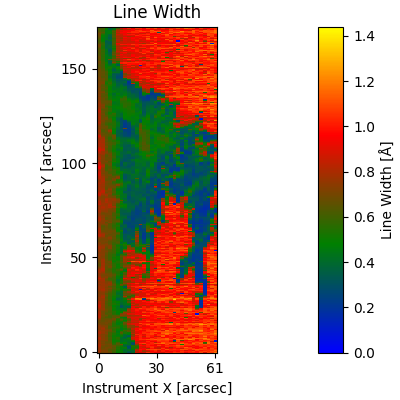
\includegraphics[width=0.5\linewidth]{./01Observations/figs/20180419/fwhmex.png} 
    \caption{\mgii~h Line Width map of raster 15 without the filter applied. The structure of the prominence is clearly distinguishable from the corona.}
    \label{fwhmex}
\end{figure}
\section{Concluding Remarks}

The prominence of 2018-04-19 is very dynamic with many flows and morphological changes through the IRIS observations. The line core shift from the quantile method demonstrates that the prominence is mainly dominated by redshifted flows relative to the solar disc. The large values of recovered asymmetry appear to be a by-product of spectral profiles with large line core shift interacting with the optical depth of the occulting plasma resulting in the absorption of parts of the line profile, exaggerating the asymmetry. This also affects the line core shift measurements, as the quantile method now overestimates the line core shift. The distribution of line core shifts found is different for \mgiihk{}, respectively.  This could be a result of \mgii~h generally having a smaller line width compared to \mgii~k or opacity effects. The prominence displayed a diverse range of line profile shapes, but was dominated by single peaked profiles due to the low column mass of the upper structure. Asymmetry is usually caused by the existence of multiple threads of different doppler velocity along the line of sight. If they are close enough in velocity, they will form what appears to a be a single asymmetric profile. This is another reason to only trust velocities where lower asymmetry is found. 

From these measurements that we can deduce directly from observations, very few conclusions can be drawn about the plasma conditions. This is where modelling is required to further our understanding of how these lines are formed, and what we can then further infer about our observations. 
\chapter{Novel \mgii\ Line Profile Comparisons from 1D NLTE Modelling}\label{Chap:prom}


Simulation and modelling are some of the most powerful tools that we have when facing solar atmospheric problems. We cannot directly deduce the conditions of the solar atmosphere with only observations: we need to do some degree of forward modelling. In this chapter we will explore the use of a novel method to find the internal properties of solar prominences. We match line profiles from 1D radiative transfer modelling with that of observed line profiles and use a measure of root mean squared difference (RMS) to evaluate the goodness of fit. From this, we are able to say how confident we are with our matched line profiles and produce maps of the properties of the considered prominence. In this chapter, we will use the 1D non-local thermodynamic equilibrium (NLTE) radiative transfer (RT) code PROM (see \sect{promintro}) to generate models which we wish to match with observation.

\section{Rolling Root Mean Squared (rRMS)}
\textit{The content of this section is based on work presented in section 4 of \cite{peat_solar_2021}.}
\label{rrms}

With these models, we can attempt to invert the solar atmosphere with a grid search. In a grid search, a large group of models of differing parameters is run and then the outputs from the models are subject to some statistical test to determine the model which most closely resembles the observation. In past studies using \ion{Mg}{ii}~h\&k, such as \cite{ruan_diagnostics_2019} and \cite{zhang_launch_2019}, the statistical test employed only concerned the integrated intensities of the lines. In \cite{ruan_diagnostics_2019}, the models and the data were only qualitatively compared by plotting the observed and modelled integrated intensities of \mgii~k against \ha, and  \mgii~h against \ha. It was concluded that these relationships behaved in a consistently similar manner. In \cite{zhang_launch_2019}, the statistical test used was a root mean squared difference (RMS) minimisation between the integrated intensities of the modelled and observed \mgii~h\&k line profiles.

However, these methods discard the most important result of the simulation: the line profiles themselves. It is easy to envision a scenario in which a double peaked profile has the same integrated intensity as a single peaked profile, or vice versa. Directly comparing the modelled line profiles to the observed line profiles allows us to gain a more quantitative result; moreover, we can set a limit on our statistical measure to say whether the fit is acceptable or otherwise. \cite{heinzel_understanding_2015} fitted a computed \mgii\ line profile to the mean of six observed line profiles, but did not extend this idea to every line profile in the observation. Work to fit computed line profiles to every pixel of an observation (on the order of hundreds of thousands of line profiles) by the line shapes seems to have not been undertaken. One of the reasons for this could be that the problem is quite computationally taxing. 

For this problem I developed Rolling RMS (rRMS), which later became Cross RMS (xRMS) where the roll was replaced with a cross-correlation. Currently this works with IRIS data, but could be generalised to work with any spectrograph. Before modelled line profiles can be matched, they first had to be interpolated down to the spectral resolution of the IRIS spectrograph. The spectral pixel resolution of the NUV observations used here is 51~m\AA, while our models have a resolution of 3~m\AA. Initially, this was done through the use of fourth-order weighted essentially non-oscillatory interpolation \citep[WENO4; ][]{janett_novel_2019}\footnote{The Python implementation used can be found at \href{https://github.com/Goobley/Weno4Interpolation}{https://github.com/Goobley/Weno4Interpolation} or installed via pip}, however, it was later found that linear interpolation offered similar results at a greater computational speed. The interpolation was performed such that the models remained symmetrical about their line core. After the models were interpolated down to 51~m\AA, both the models and the data were interpolated up to a resolution of 25.5~m\AA. This was done such that if the line core lay between two spectral pixels in the data, the model profile could be better centred on the data. Tests where the models and data were interpolated up to resolutions of 17~m\AA\ and 12.75~m\AA\ showed that these offered little to no increase in number of matches, whereas the run time increased. The data was trimmed to two separate 3~\AA\ windows centred on the rest wavelengths of \mgii~h\&k, respectively. This spectral window is considerably larger than the wavelength range of the models, and so they are padded with zeros to match the wavelength range of the data. Then, to account for the background level in the observations, the mean of the intensity between 2797.85~\AA{} and 2802.03~\AA{} of the observation is added to the model before matching. These two values are at the edges of the aforementioned 3\AA{} windows. The model line profiles were then rolled through these 3\AA{} wavelength windows measuring the RMS at every position (defined by \eq{rmseq}). See Fig. \ref{fig:rrms} for a visual representation of the algorithm.
\begin{equation}
    \text{RMS}(\Delta\lambda)=\sqrt{\frac{1}{n}\sum_n\left(\text{data}-\text{model}\right)^2},
    \label{rmseq}
\end{equation}
\begin{figure}
    \centering
    \includegraphics*[width=.7956\linewidth]{./02Modelling1D/figs/20180419/rrms1.png}\\
    \includegraphics*[width=.7956\linewidth]{./02Modelling1D/figs/20180419/rrms2.png}
    \caption[Example of rRMS working.]{Example of rRMS working. These panels are in sets of two; with the upper of each set (orange) rolling over the data (blue) and the bottom of each set the current RMS at that position (dotted orange), the future RMS measurements (transparent blue), and the RMS measured up to that point (solid orange). This demonstrates the method employed by the algorithm to find the best fitting location of the currently considered model profile. The model profile is rolled one spectral pixel at a time across the entire wavelength window measuring the RMS at each pixel location.}
    \label{fig:rrms}
\end{figure}

where $n$ is the number of data points in wavelength space. The pixel shift required to produce the lowest RMS is assumed to be the best matching position for that model. The RMS and its associated pixel shift are saved, then the next model is compared. This is done independently for both \mgii~h\&k, then their RMS values are added together and the model that produces the lowest total RMS for that pixel is selected as the model most indicative of the plasma parameters in that pixel. This is done in vectorised fashion through the use of the Numpy Python library \citep{harris_array_2020}, greatly increasing the speed of the computation. Additionally, this was run in parallel over the 18 rasters of the observation on a machine with a dual socket motherboard with two Intel Xeon E5-2697 v4s giving a wall time\footnote{The time taken for the program to execute in real time (i.e., measured by a clock on a wall).} of approximately 1 hour and 30 minutes, and a CPU time\footnote{The sum of the run time on every CPU core/thread.} of 27 hours.

\subsection{Prominence of 2018 04 19}
\label{20180419}
As discussed in section \ref{20180419main}, a prominence appeared off of the south-western solar limb on the 19 April 2018. The observations carried out by IRIS allowed us to develop the aforementioned tool, rRMS. Using the iteration of PROM presented in \cite{levens_modelling_2019}, we generated 1007 model prominences; 252 isothermal and isobaric models, and 755 models with a PCTR. The parameters of these can be seen in table \ref{modeltable}. The parameters here have 1008 unique combinations, however, one of the models did not converge, leaving us with 1007. Here we have one value for both the microturbulent velocity and height parameters. The value used for the microturbulent velocity is the generally accepted value expected to be found in the main bulk of a prominence \citep{labrosse_physics_2010}, however, the latter has a more nuanced argument. Since height is something that can be measured directly from observation, it appears to be something that we can simply feed into our calculations, where every pixel has a height associated with it. In theory, this is  a good idea, but in practice, every new value added to for $H$ will increase the size of the grid by a further 1007 (or 1008 if that one model now converges with a different height). If we assume every pixel in a raster is of the same altitude, we would have to create 32~224 models in total. This is even greater than the extended grid of 23~940 discussed in \sect{xrms}. This may have an effect on the solutions recovered as all of the pixels are not at a height of 10~000~km. At different altitudes, models of similar parameters exhibit lower intensities at higher altitudes. This may mean that higher features may be hotter and/or more dense, and lower features may be cooler and/or less dense. Slab width may also be affected in similar ways.


\begin{table}
    \centering
    \begin{tabular}{ccc}
    \hline \hline
    Parameter & Unit  & Value                                                                \\ \hline\hline
    $T_{\text{cen}}$   & K              & \begin{tabular}[c]{@{}c@{}}6000, 8000, 10~000, 15~000, \\ 20~000, 25~000, 30~000, \\ 35~000, 40~000\end{tabular}         \\
    $T_{\text{tr}}$    & K              & 100000 \\
    $p_{\text{c}}$   & dyne cm$^{-2}$ & 0.01, 0.02, 0.05, 0.1, 0.2, 0.5, 1                                                                    \\
    $p_{\text{tr}}$     & dyne cm$^{-2}$ & 0.01                                                                   \\
    Slab Width & km             & 200 -- 124100                                                                                                     \\
    M         & g cm$^{-2}$    & $3.7\times10^{-8}$--$5.1\times10^{-4}$                                                                            \\
    $v_T$ & km~s$^{-1}$ & 5 \\
    $H$ & km & 10~000 \\ 
    $\gamma$  &                & 0, 2, 5, 10  \\ \hline
    \end{tabular} 
    \caption{Parameters of the models. There are 1008 unique combinations here, however, one of the models did not converge, so there are only 1007.}
    \label{modeltable}
\end{table}


After rRMS was run, twelve line profiles were observed by eye and classified as a satisfactory match or unsatisfactory match, and their RMS was noted. These profiles were taken from the three main stages of the prominence described in \chap{Chap:obs} from both the body and the extending arm. An example of four of these can be seen in Fig. \ref{egpx}. A $\chi^2$ statistic (see \eq{chi2}) was also considered for this, but the values of $\chi^2$ were exceedingly high for the number of degrees of freedom of this problem (approximately 233 -- the number of wavelength points). 
\begin{equation}
    \chi^2=\sum_n\frac{\left(\text{data}-\text{model}\right)^2}{\text{model}}
    \label{chi2}
\end{equation}
This is likely due to the way in which the models are padded to be 3\AA{} wide. There are significantly more padded points than points in the model itself, this is clearly seen in \fig{fig:rrms}. The model is essentially padded by the mean of the signal between 2797.85~\AA{} and 2802.03~\AA{} of the observation. This means that we are comparing the background to the mean of itself. This causes the $\chi^2$ to be very large. This would cause us to revert back to having to check our matches by eye to find a good $\chi^2$ value. Additionally, if we instead limit the range of our $\chi^2$ calculation to only the region where the model is valid, we recover strange results. Matches that by eye are bad are sometimes found to be good via the $\chi^2$ statistic. This is because some observed line profiles are wider than the range in which the model is valid. By limiting the calculation to this range, the wings of these observations are ignored, leading to an erroneous $\chi^2$ which reports the fit to be good.

From this, we can decide on a threshold RMS value where those below the threshold are considered satisfactory matches and those above the threshold are considered unsatisfactory. This gives us a statistical test to determine the goodness of the found fits. It should be stressed that this method can only perform as well as how well the model grid represents the data. This RMS limit was found to be 15~000, leading to 49\% (35617/72536) of the matches being considered as satisfactory. 62\% of the satisfactory models contained a PCTR showing the importance of its inclusion when simulating \mgii~h\&k. There appears to be a weak correlation between satisfactory fits and higher k/h ratio (see Fig. \ref{khandgoods}). In the optically thin regime, the ratio of the integrated intensities of two lines from the same ion tends towards the ratio of their respective oscillator strengths. The oscillator strengths of \mgii~h\&k are 0.300 and 0.601, respectively \citep{theodosiou_accurate_1999}, leading  to the ratio of the oscillator strengths of \mgii\ k to \mgii{} h to be approximately 2. Therefore, Fig. \ref{khandgoods} suggests that we are more likely to find good matches in areas of lower optical depth. 




\begin{figure}
    \centering
    \resizebox{\hsize}{!}
    {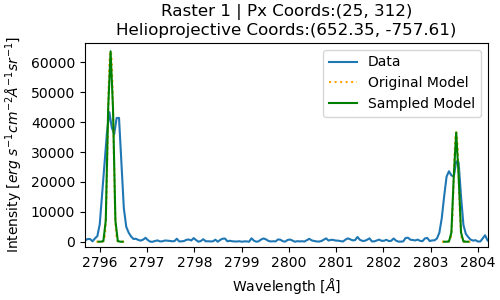
\includegraphics[width=0.49\linewidth]{./02Modelling1D/figs/20180419/inv/bad5.png}
    \includegraphics[width=0.49\linewidth]{./02Modelling1D/figs/20180419/inv/bad1.png}
    }
    \resizebox{\hsize}{!}
    {\includegraphics[width=0.49\linewidth]{./02Modelling1D/figs/20180419/inv/good7.png}
    \includegraphics[width=0.49\linewidth]{./02Modelling1D/figs/20180419/inv/good3.png}
    }
    \caption[Four of the twelve matches investigated to set a threshold for the RMS of models found by the algorithm.]{Four of the twelve matches investigated to set a threshold for the RMS of models found by the algorithm. The top two are unsatisfactory matches and the bottom two are satisfactory matches. These plots are from \cite{peat_solar_2021}}
    \label{egpx}
\end{figure}


\begin{figure}
    \centering
    \includegraphics[width=0.3\linewidth]{./02Modelling1D/figs/20180419/kh14.png}
    \includegraphics[width=0.3\linewidth]{./02Modelling1D/figs/20180419/goodbad14.png}
    \caption[k/h ratio and satisfactory fits of raster 15. This demonstrates the weak correlation between high k/h ratio and satisfactory fits.]{\textit{Left}: k/h ratio of raster 15. \textit{Right}: Satisfactory fits of raster 15. This demonstrates the weak correlation between high k/h ratio and satisfactory fits. Raster 15 was taken between 18:08 and 18:25 UTC. These plots are from \cite{peat_solar_2021}}
    \label{khandgoods}
\end{figure}

For the results, we will discuss mean pressure and temperature as opposed to the central pressures and temperatures. This gives us a better view of the conditions inside the plasma.
Mean pressure is defined as,
\begin{equation}
    \overline{p}=\frac{1}{M}\int_0^M 4p_c\frac{m}{M}\left(1-\frac{m}{M}\right)+p_{\text{tr}}\hspace{0.1cm}dm,
    \label{meanpresint}
\end{equation}
which evaluates to,
\begin{equation}
    \overline{p}=\frac{2p_{\text{cen}}+p_{\text{tr}}}{3}.
    \label{meanpres}
\end{equation}
Mean temperature is defined as,
\begin{equation}
    \overline{T}=\frac{2}{M}\int_0^{\frac{M}{2}}T_{\text{cen}}+(T_{\text{tr}}-T_{\text{cen}})\left(1-4\frac{m}{M}\left(1-\frac{m}{M}\right)\right)^\gamma dm,
    \label{meantempint}
\end{equation}
which evaluates to
\begin{equation}
    \overline{T}=\frac{2\gamma T_{\text{cen}}+T_{\text{tr}}}{2\gamma+1}.
    \label{meantemp}
\end{equation}
The integral in \eq{meanpresint} is between 0 and $M$ but \eq{meantempint} is between 0 and $M/2$. The prominence is symmetrical around $M/2$, so finding the mean between 0 and $M$ is analogous to the mean between 0 and $M/2$. These bounds are chosen such that they simplify the algebra in the result of the integral.

Figs \ref{mainresults} and \ref{subresults} show the diagnostic results from rRMS. Raster 15 is chosen as the example raster in Fig \ref{subresults} solely due to the field of view being mostly covered by the prominence in this raster.

The mean pressure appears to remain stable over the entire observation, showing small fluctuations between 0.18 and 0.26~dyn~cm$^{-2}$. Towards the centre of the prominence, we find pressures of 1 dyn~cm$^{-2}$. A pressure of 1 dyn~cm$^{-2}$ is at the upper limit of pressures expected to be seen in prominences \citep{labrosse_physics_2010}. However, these high pressures also correlate with areas of unsatisfactory fits. As noted in \chap{Chap:obs}, these are where the most complicated line profiles seem to appear. High pressures can lead to broader line profiles, and this is why rRMS has selected these profiles as a best fit. 1D models are unable to create complicated line profiles like this because the geometry in reality cannot be represented in 1D. The outside and edges of the prominence generally exhibit lower pressures as we move through the PCTR from the core to the low pressure corona \citep{aschwanden_physics_2004}.

As with the mean pressure, the mean temperature also appears stable. On average, the temperature remains between 7800 and 11~500~K. This is consistent with results one would expect. \mgii~h\&k is said to probe the upper photosphere to the upper chromosphere \citep{depontieu_interface_2014} and a prominence is expected to exhibit a range of chromospheric to transition region temperatures. As we approach the edge of the prominence, higher temperatures are observed. This is consistent with where we would expect to observe the PCTR, and therefore higher temperatures, in the plane-of-sky. It could also be that we are intercepting more PCTR material along the line of sight nearer to the edges of the prominence. This would explain why so many fits towards the outside of the prominence have a non-zero gamma value. The arm seen to extend from the prominence near the end of the observations in raster 15 appears to be a hot and tenuous structure reaching temperatures of 4 to 5$\times10^4$~K.

Many of the good fits require a non-zero value of $\gamma$, especially those near the outside of the prominence where higher temperatures are reached. This demonstrates the value of including a PCTR in prominence models. The mean temperatures we find are greater than those found in past \mgii\ studies, such as the study by \citep{zhang_launch_2019}. However, the authors of these past studies did not include a PCTR, they only considered isothermal and isobaric models. In future, we suggest implementing a finer $\gamma$ grid to gain better resolution of the structure of the PCTR surrounding the prominence.

\begin{figure}
    \centering
    \includegraphics*[width=0.25\linewidth]{./02Modelling1D/20180419/outputs/mean_temp/0.png}
    \includegraphics*[width=0.25\linewidth]{./02Modelling1D/20180419/outputs/mean_pres/0.png}
    \includegraphics*[width=0.25\linewidth]{./02Modelling1D/20180419/outputs/gamma/0.png}
    \\
    \includegraphics*[width=0.25\linewidth]{./02Modelling1D/20180419/outputs/mean_temp/11.png}
    \includegraphics*[width=0.25\linewidth]{./02Modelling1D/20180419/outputs/mean_pres/11.png}
    \includegraphics*[width=0.25\linewidth]{./02Modelling1D/20180419/outputs/gamma/11.png}\\
    \includegraphics*[width=0.25\linewidth]{./02Modelling1D/20180419/outputs/mean_temp/14.png}
    \includegraphics*[width=0.25\linewidth]{./02Modelling1D/20180419/outputs/mean_pres/14.png}
    \includegraphics*[width=0.25\linewidth]{./02Modelling1D/20180419/outputs/gamma/14.png}
    \caption[Evolution of mean temperature, pressure, and gamma in the prominence through the main three stages of its evolution, identified in section \ref{20180419main}.]{Evolution of mean temperature, pressure, and gamma in the prominence through the main three stages of its evolution, identified in section \ref{20180419main}. The left and mid columns, and bottom right plot are from \cite{peat_solar_2021}}
    \label{mainresults}
\end{figure}

\begin{figure}
    \centering
    \includegraphics*[width=0.3\linewidth]{./02Modelling1D/20180419/outputs/mnne/14.png}
    \includegraphics*[width=0.3\linewidth]{./02Modelling1D/20180419/outputs/ion_deg/14.png}
    \includegraphics*[width=0.3\linewidth]{./02Modelling1D/20180419/outputs/cmass/14.png} 
    \caption[Mean electron density, ionisation degree, and column mass of the prominence at the culmination of the three stages defined in section \ref{20180419main}.]{Mean electron density, ionisation degree, and column mass of the prominence at the culmination of the three stages defined in section \ref{20180419main}. These plots are from \cite{peat_solar_2021}}
    \label{subresults}
\end{figure}


The column mass found suggests that the extensions of the prominence are of relatively low mass. Where we find unsatisfactory matches, the mass density is seen to be much higher. We also see \ha\ emission in this area, and \ha\ is known to require denser areas to be seen. The unsatisfactory fits here are mainly due to the single slab nature of the 1D modelling. As discussed, we see several threads along the line of sight in this area. A single slab model can only apply, when there are several threads, if the threads are co-moving, resulting in a single line profile. The arm seen to extend near the end of the observations is seen to be of relatively low mass. This explains the single peaked profiles seen in the arm. The intensity of the line core of \mgii~h\&k is anticorrelated with optical depth, which further explains the correlation between single peaked profiles and low mass density \citep{leenaarts_formation_2013}.

On the whole, the prominence appears to have an electron density less than $0.6\times10^{11}$~cm$^{-3}$, with few areas exceeding $1\times10^{11}$~cm$^{-3}$ (Fig. \ref{subresults}). The arm is seen to be of comparatively low electron density, although it is high temperature. However, it is also of low pressure, which can explain this disparity. 

Ionisation degree is defined by the mean number density of \ion{H}{ii} ($n_\text{HII}$) to the mean number density of \ion{H}{i} ($n_\text{HI}$) \citep{tandberg-hanssen_nature_1995}. Past works have assumed that the mean number of electrons ($n_\text{e}$) is equal to the mean number of protons ($n_\text{p}$), which is equal to the mean number density of \ion{H}{ii}. The mean number of \ion{H}{i} is also thought to be dominated by the mean number density of ground state Hydrogen ($n_\text{H0}$), such that,

\begin{equation}
    \frac{n_\text{HII}}{n_\text{HI}}\approx\frac{n_\text{p}}{n_\text{H0}}\approx\frac{n_\text{e}}{n_\text{H0}}.
\end{equation}

However, the assumption that $n_\text{e}\approx n_\text{p}=n_\text{HII}$ does not hold in PROM as not all of the electrons are liberated from \ion{H}{i}. There is a fixed percentage contribution from other species, mainly helium. These `non-hydrogen' electrons contribute greatly to $n_\text{e}$ at high temperatures. The right panels of Fig. \ref{iondeg} shows how this assumption breaks down at higher temperatures. Above 30~000~K, $n_\text{HII}$ is overestimated by 20\% by this metric. So here, we focus on the definition from \cite{tandberg-hanssen_nature_1995}. Parts of the prominence show a very high ionisation degree when compared to past studies. \cite{vial_solar_1998} stated that the ionisation degree in a prominence does not dramatically change with temperature, given that the density is low. This statement was grounded in studies by \cite{gouttebroze_hydrogen_1993} and \cite{heinzel_theoretical_1994}. However, these studies did not consider temperatures above 15~000~K and did not include a PCTR. The left of Fig. \ref{iondeg} shows that above this temperature, ionisation degree increases exponentially. Additionally, at this temperature, the overestimation of $n_\text{HII}$ when it is assumed to be equal to $n_\text{e}$, is only approximately 7\%. This could very easily go unnoticed. In past studies using isothermal and isobaric models, ionisation degree was not thought to rise above 10. However, areas of high ionisation degree (see Fig. \ref{subresults}), strongly correlate with areas of non-zero $\gamma$. This demonstrates that the inclusion of a PCTR can dramatically influence the value of the ionisation degree.



\begin{figure}
    \centering
    \includegraphics*[width=0.4\linewidth]{./02Modelling1D/figs/20180419/ideg_temp_new.png}
    \includegraphics*[width=0.4\linewidth]{./02Modelling1D/figs/20180419/excess_electrons.png}
    \caption[Exponential rise in ionisation degree above 30~000~K and how the assumption that $n_\text{e}\approx n_\text{HII}$ breaks down at high temperatures.]{\textit{Left}: Exponential rise in ionisation degree above 30~000~K. \textit{Right}: How the assumption that $n_\text{e}\approx n_\text{HII}$ breaks down at high temperatures. These plots are from \cite{peat_solar_2021}.}
    \label{iondeg}
\end{figure}

As an added consequence of rRMS, we also obtain line of sight Doppler velocities as we recover the pixel location in wavelength where the lowest RMS is found. This allows us to create Doppler maps which can be compared to the Doppler maps recovered from the quantile method shown in \sect{velsect} to demonstrate that the algorithm is functioning correctly. The resolution of these line core shifts is approximately 2.7~km~s$^{-1}$. This number is from the minimum measurable line core shift by the procedure. This is equal to the wavelength resolution of the observations divided by the number of sub-pixels plus one. 

Fig. \ref{vels} shows the line core shift found via the quantile method and that recovered by rRMS. The Doppler maps of the top of this figure appear to qualitatively agree. With the other diagnostics, there is uncertainty in the recovered value where unsatisfactory fits are found. While these models do not represent the conditions of the prominence plasma, the fit found by the procedure should still find a good measure of the line core shift; regardless of how bad the fit is. This is because the lowest RMS is mostly found when the model profile is centred on the data profile. Due to this, we can reasonably trust the line core shifts recovered by rRMS, even where unsatisfactory fits are found.
The histograms for the recovered line core shift from rRMS in Fig. \ref{vels} have fewer bins than that of the line core shift measured by the quantile method. This is because the velocity resolution of the results of the quantile method is essentially infinite, but the resolution of the recovered line core shifts is only 2.7~km~s$^{-1}$, as previously discussed. Both of these distributions approximate well to Gaussians. The fit to the histograms obtained via the quantile method are centred on a line core shift of 8.20~km~s$\pm$5.98\kms and 5.20$\pm$6.61\kms for \mghk, respectively. Those recovered via rRMS are centred on a line core shift of 5.3~km~s$^{-1}$ and 5.6~km~s$^{-1}$ with standard deviations of 9.8~km~s$^{-1}$ and 10.2~km~s$^{-1}$ for \mghk, respectively. Due to the limited resolution of the line core shift recovered by rRMS, a value of $\pm1.35$~km~s$^{-1}$ is given as an estimate of the uncertainty of these values. This value is half of the minimum recoverable line core shift by rRMS. The central line core shift of \mgii~k measured by the quantile method is within the uncertainty of the line core shift recovered from rRMS. However, this is not true with the line core shift of \mgii~h. This is believed to be due to the asymmetry bias discussed in \sect{velsect} but it is not clear why only \mgii~h is affected by this. This could be a result of \mgii~h generally having a smaller line width compared to \mgii~k or opacity effects.

\begin{figure}
    \centering
    \includegraphics*[width=0.4\linewidth]{./02Modelling1D/figs/20180419/quantdopp.png}
    \includegraphics*[width=0.4\linewidth]{./02Modelling1D/figs/20180419/rolldopp.png}\\
    \includegraphics*[width=0.3\linewidth]{./02Modelling1D/figs/20180419/hvelocities.png}
    \hspace{1cm}
    \includegraphics*[width=0.3\linewidth]{./02Modelling1D/figs/20180419/hvelocitiesfound.png}\\
    \includegraphics*[width=0.3\linewidth]{./02Modelling1D/figs/20180419/kvelocities.png}
    \hspace{1cm}
    \includegraphics*[width=0.3\linewidth]{./02Modelling1D/figs/20180419/kvelocitiesfound.png}
    \caption[Doppler velocities found using the quantile method and Doppler velocities recovered from rRMS.]{\textit{Left:} Doppler velocities found using the quantile method. \textit{Right:} Doppler velocities recovered from rRMS. The dashed line represents a line core shift of 0~km~s$^{-1}$ and the orange line is a Gaussian fit. These plots are from \cite{peat_solar_2021}}
    \label{vels}
\end{figure}
\newpage
\section{Cross Root Mean Squared (xRMS)}
\label{xrms}
\textit{The content of this section is based on work presented in Peat et al. (in prep.).}

Since the publication of \cite{peat_solar_2021}, rRMS has been modified and renamed. It is now called Cross(-correlation) Root Mean Square Difference (xRMS). The main difference between rRMS and xRMS is that the `roll' is predetermined by a cross-correlation, hence the name change. A cross-correlation is naturally produced when attempting to minimise (or maximise) a mean square \citep{elliott_handbook_1987}, and therefore also when minimising a root mean square. Additionally, \cite{brown_doppler_2016} demonstrated that a cross correlation could be employed to find the line core shift of the Lyman lines in solar flares. As the rolling aspect of rRMS was essentially measuring the line core shift, it was decided that computation time could be greatly improved by the introduction of a cross-correlation to predetermine the line core shift. After the cross-correlation is computed, the line profiles are then rolled to their respective line core shift, and the RMS was measured. This improved the run time by a factor of approximately 10. This final roll was then determined to be the new bottleneck to the algorithm, and so this was also improved upon. As a model profile is being matched, a reference padded profile (rpp) is created. This rpp is the considered model profile padded on both sides by zeroes the length of the difference between the length of the data array and the model array. This allows us to take slices of the rpp identical to the result of a would-be roll. Taking slices of an array does not create a new array, and only a new pointer (or reference in Python) which is considerably faster. This removed the need for rolled model arrays to be created, improving the run time by a further factor of approximately 2. xRMS and rRMS give the same results, but due to the optimisations introduced, xRMS is much faster. Running the same 1007 model grid on the same data as presented in \cite{peat_solar_2021}, but using xRMS, on the same dual socket motherboard machine with two Intel Xeon E5-2697 v4s, gives a wall time of approximately 6 minutes and 30 seconds, and a CPU time of 1 hour and 57 minutes. Due to this great improvement in computation time, this allows us to use a much larger grid of models.

In addition to the faster computation time, xRMS supplies us with an estimate of the errors on our inversion. It does this by saving the 20 next best fitting models alongside the best fitting model. Then, of these secondary models, it removes those whose RMS is lower than the threshold value as defined previously. This is followed by finding the maximum difference between the `best fit' diagnostics and the remaining good secondary fit diagnostics. These values are then divided by the `best fit' value to recover fractional errors. This is done to give a better indication of the range of values of good, but not best, fits that can be found. These fractional errors are how the uncertainty will be presented in plots later in this section. This maximum difference which makes up the error need not be from the same model. To be conservative, the error is the greatest difference produced by any of the secondary models. For example, a pixel may not necessarily use the same model for its pressure uncertainty and temperature uncertainty.
 
\subsection{Prominence of 2018 04 19: Revisited}

To exhibit the efficacy of the new algorithm, we will use the prominence used to demonstrate rRMS in \sect{20180419} to illustrate how our matches improve with a greater set of models.

As mentioned above, here can we employ a much larger grid of models than used previously due to the increase in computation offered by xRMS. Additionally, we introduce the parameter $v_\text{rad}$. This is the radial (outward) velocity. This allows us to introduces Doppler dimming into our models. In total, there are 23~940 models in our new grid, this includes the previous 1007 models used in \sect{20180419}. See Table \ref{23940table} for the range of parameters present in the models. Please note that these values are not all uniquely combined.
\begin{table}[]
    \centering
    \begin{tabular}{ccc}
    \hline\hline
    Parameter  & Unit                & Value                                                                                                                                                        \\ \hline
    $T_\mathrm{cen}$  & K                   & \begin{tabular}[c]{@{}c@{}}6000, 8000, 10~000, 12~000, 15~000,\\ 20~000, 25~000, 30~000, 35~000, 40~000\end{tabular} \\
    $T_\mathrm{tr}$   & K                   & 100~000                                                                                                                                                 \\
    $p_\mathrm{cen}$  & dyne~cm$^{-2}$ & 0.01, 0.02, 0.05, 0.1, 0.2, 0.5, 1                                                                                                                           \\
    $p_\mathrm{tr}$   & dyne~cm$^{-2}$ & 0.01                                                                                                                                                         \\
    Slab width & km                  & 45-124~100                                                                                                                                              \\
    M          & g~cm$^{-2}$    & $3.7\times10^{-8}-5.1\times10^{-4}$                                                                                                                          \\
    $v_{T}$    & km~s$^{-1}$    & 5, 8, 13                                                                                                                                                     \\
    $v_\mathrm{rad}$  & km~s$^{-1}$    & \begin{tabular}[c]{@{}c@{}}0, 2, 4, 6, 8, 10, 20, 40,\\ 60, 80, 100, 150, 200\end{tabular}                                                                   \\
    H          & km                  & 10~000, 30~000, 50~000                                                                                                                        \\
    $\gamma$   &                     & 0, 2, 4, 5, 10                                                                                                                                               \\ \hline
    \end{tabular}
    \caption[The considered model parameters to be used in xRMS.]{The considered model parameters to be used in xRMS. Not all of these parameters are uniquely combined; there are 23940 total model profiles. Amongst these models are the original 1007 from \sect{20180419}.}
    \label{23940table}
\end{table}
The results from xRMS can be seen in \fig{20180419rresults}. As the grid of models was increased, even though the previous 1007 models were coarsely separated, the cut off value did not change. After investigating the same 12 profiles, the cut off value was once again decided to be 15000. We now achieve 55.14\% (39450/71548) satisfactory matches. The total number of pixels is different with xRMS than rRMS as the updated version of the filter discussed in \sect{20180419main} is used in xRMS but not in rRMS. 

As noted in \sect{20180419main}, the prominence displays an array of interesting line profiles. With these new diagnostics, we can explore some of them in more detail. In \fig{2structs}, shows one of the unsatisfactory matches. However, it could be argued that this is satisfactory as this is not a double peaked profile, but two structures. The main drawback of this method is that it assumes single structures along the line of sight. In the future, it could be possible to allow for multi-structure solutions, but this would almost double the required computation time, so this method may be reaching its limit. From the matching model, we can see that the optical depth of the fit structure is $0.97$ and $1.90$ for \mgiihk{}, respectively, and the k/h ratio is approximately $1.71$. Therefore, it is safe to say that this structure is mostly optically thin. In this case, we would be justified in trying to fit a second peak as if the first was not there. From just looking at the line profiles and the model line profiles, I would expect a similar, if not the same, model to fit this secondary peak. There are many other line profiles like this in the prominence, but this is the most apparent example. In \sect{2dinvert} we attempt to invert this spectrum using stacked 2D models.

\begin{figure}
    \includegraphics[width=\linewidth]{./02Modelling1D/figs/lineprofs/r15y13x207.png}
    \caption[The \mgiihk{} spectra from the raster taken from 18:25:09~UTC.]{The \mgiihk{} spectra from the raster taken from 18:25:09~UTC. The orange cross indicates the location this spectra is taken from. The model found to match by xRMS here has the following parameters, $T=8000$~K, $p=0.02$\dyncm{}, Slab Width$=200$~km, $v_T=8$\kms{}, $H=10000$~km, $v_\text{rad}=80$\kms{}, and $\gamma=0$, with associated Doppler velocities of $v_{dh}=-27.0$\kms{} and $v_{dk}=-27.0$\kms{}.}
    \label{2structs}
\end{figure}

\fig{similar} shows two spectra of similar parameters. The difference in microturbulent velocity is apparent due to their difference in line width. These two spectra come from different parts of the prominence. The top panel is from the middle of the main extension, and the bottom panel from one of the smaller extensions from the main body. Although they are in very different locations, they both have the same central temperature, and mean temperature (32000K). Their pressures, however, are different. The pressure of the main extension is four times higher than that of the smaller extension. This is not surprising, as the main extension is comprised of a larger volume than that of the smaller extension. Their measure of radial velocity can also tell us more about the velocity perpendicular to the solar limb. The main moving faster than the small extension. This is consistent with observation, as the smaller extensions are seen to move slower than the main extension in SJI movies.
\begin{figure}
    \includegraphics[width=\linewidth]{./02Modelling1D/figs/lineprofs/r12y23x245.png}
    \includegraphics[width=\linewidth]{./02Modelling1D/figs/lineprofs/r17y15x238.png}
    \caption[The \mgiihk{} spectra from two raster taken at different times, 17:34:54~UTC and 18:58:40~UTC]{The \mgiihk{} spectra from two raster taken at different times, 17:34:54~UTC and 18:58:40~UTC for the top and bottom panel respectively. The orange cross indicates the location this spectra is taken from. The model found to match by xRMS here has the following parameters, I will omit the PCTR variables as they can only be one number (see Table \ref{23940table}), \\\textit{Top}: $T_\text{cen}=15000$~K, $p_\text{cen}=0.20$\dyncm{}, Slab Width$=1148$~km, $v_T=13$\kms{}, $H=10000$~km, $v_{\text{rad}}=80$\kms{}, and $\gamma=2$. With associated Doppler velocities of $v_{dh}=5.22$\kms{} and $v_{dk}=5.23$\kms{}. \\\textit{Bottom}: $T_\text{cen}=15000$~K, $p_\text{cen}=0.05$\dyncm{}, Slab Width$=2640$~km, $v_T=5$\kms{}, $H=50000$~km, $v_{\text{rad}}=60$\kms{}, and $\gamma=2$. With associated Doppler velocities of $v_{dh}=13.84$\kms{} and $v_{dk}=13.88$\kms{}.}
    \label{similar}
\end{figure}

As a whole, in comparison to our results with a smaller set of models, we see a much more striking temperature structure. Compared to the mean temperatures seen in the previous result, they are much higher here. The temperature structure seems more homogeneous, but the highest temperatures are still found in the arm.
The fractional errors, however, are mostly between 0 and 3. The distribution of recovered pressures is also different. The higher microturbulent velocities have allowed a better match at the centre of the prominence than those of high pressure. However, we still do not find satisfactory matches in this area due to the multiple structures seen in many pixel locations. The areas we find good matches in correlate with areas of lower pressure. Before, we had many regions in the prominence where $\gamma=10$, but now there are none, with $\gamma=4$ and $\gamma=2$ appearing in these high temperature areas. However, the uncertainty shows that gamma could be up to two times higher in the majority of the regions where it was previously found to be 10. The blank spaces in the gamma uncertainty map are where an isothermal and isobaric model was found to be the best fit. Calculating the fractional difference in these locations is meaningless, and so they are discarded. Like before, our satisfactory matches correlate weakly with high k/h ratio. Our lowest errors (bottom of \fig{20180419rresults}) correlate with both of these graphs. 

\begin{figure} 
    \centering
    \includegraphics*[width=\linewidth]{./02Modelling1D/20180419r/fullfig.png}
    \caption[Mean Temperature, Pressure, and Gamma Results from xRMS for the prominence of 2018 04 19]{Mean Temperature, Pressure, and Gamma results for the middle of the three stages identified in the prominence. \textit{Left}: Mean temperature. \textit{Mid}: Mean pressure. \textit{Right}: Gamma. \textit{Top}: The main result. \textit{Bottom}: Their fractional uncertainties.}
    \label{20180419rresults}
\end{figure}

However, presenting these as a traditional plus/minus uncertainty is perhaps not best, as 1D inversions like this can be shown to have degenerate solutions. In test 1D Markov Chain Monte Carlo (MCMC) inversions of a set of simulated (and known-parameter) \mgiihk{} line profiles show that posterior likelihoods tend to display multimodal distributions \citep{osborne_notitle_2022}\footnote{This was explored using profiles from Promweaver: \href{https://github.com/Goobley/Promweaver}{https://github.com/Goobley/Promweaver}}. The introduction of more spectral lines from different species may solve this issue of degeneracy, but has not yet been explored. 

Even though we increased our model set by a factor of 24, we only increased our matches by approximately 6\%. Although this increase is small, some parts of the prominence now have better matches than before. This increase in satisfactory matches is owed to the increase in the number of models in the grid. However, the main problem with a grid search method is that your algorithm can only perform as well as your grid represents the plasma conditions, the grid can be continually increased, but that does not mean that your matches will improve. There is only so much 1D models can do on their own. Even though we cannot satisfactorily probe the centre of the prominence with these models, we are able to diagnose the area surrounding the prominence. This gives us insight into the enigmatic PCTR. It is the reason that we find larger than expected ionisation degrees, and high temperature. The continued study of transition region lines, such as \mgiihk{}, can lead to a better understanding of how the PCTR is structured.  



\section{Concluding Remarks}

1D modelling can be a very useful tool to understand how the internal plasma parameters of a solar prominence affect the shape of its observed line profiles.
However, they are limited in their use to diagnose the internal plasma parameters from observation. Their 1D nature means that they cannot easily model the mulithreaded nature of many prominences. Additionally, they can be shown to have degeneracies in their solutions when fitting to one species. The introduction of multiple species may solve this issue, but this topic remains unexplored. Despite these limitations, they can (and have) shown us that the PCTR is very important when it comes to \mgiihk{} modelling. This is likely due to their high optical thickness which only allows us to probe the surface of the prominence and not penetrate too deeply into the body. The seemingly degenerate nature of this problem of inverting prominence atmospheres using 1D modelling motivates us to explore the applications and interpretation to be gleaned from 2D modelling. However, in future, coordinated observations of different line profiles, such as \mgiihk{} and \ha{}, could be used to further constrain the atmosphere and may solve this degeneracy problem.
\chapter{Complex Prominence Emission Through\\2D Cylindrical Radiative Transfer Modelling}\label{Chap:2DModel}

Prominences are inherently 3D structures and must be treated as such. Here we explore the use of cylindrical geometry with radiative transfer calculated along a `single slit' focused on the centre of this geometry. We can also stack several different cylinders of varying thermodynamic parameters to produce complex line profiles akin to the line profiles that 1D modelling struggles, or even fails, to model. Here we make use of the 2D NLTE RT code, RTCY described in \sect{rtcyintro}.



\section{Effects of Velocity on Line Formation}
%\section{Single Thread Simulations}
As RTCY includes a variety of velocity settings, and we can investigate how these affect the line formation. Initially we investigate the formation of the lines in the static case, as presented in \fig{fig:exhmg}. We can investigate the line formation here by consulting the corresponding Carlsson and Stein plots.

\begin{figure}
    \centering
    \includegraphics[width=\linewidth]{./03Modelling2D/figs/exmg.png}
    \caption[Output of RTCY for the h\&k lines of once-ionised magnesium.]{Output of RTCY for the h\&k lines of once-ionised magnesium. The units of the colourbars are \cgsint. The parameters of this example run are; $P=0.1$~dyn~cm$^{-2}$, $r_0=500$~km, $r_1=1000$~km, $T_0=6000$~K, $T_1=100~000$~K, $v_T=5$~km~s$^{-1}$, $\alpha=\frac{\pi}{2}$~rad and $H=10000$~km with no velocity setting active.}
    \label{fig:exhmg}
\end{figure}

\begin{figure}
    \centering
    \includegraphics[width=0.9\linewidth]{./03Modelling2D/figs/matplots/mghv0.png}
    \caption[The various plots that break down the contribution function.]{The various plots that break down the contribution function for the line at $z=0$ for the run in \fig{fig:exhmg}. The $\tau=1$ line is drawn on each of these plots in light grey, and the line profile is drawn in red. The left y axis is the distance through the prominence and is defined from the POV of the LOS. So 0 is the front of the prominence and 1 is the back. The right y axis is for the line profile.}
    \label{v0}
\end{figure}
\fig{v0} shows us this plot for \mgii~h. \mgii~k is similar to \mgii~h, and will be omitted. These plots are taken from the centre of the hypothetical slit spectrograph ($z=0$). Distance through the prominence is measured along the line of sight with $D=0$ being the front of the prominence and $D=1$ being the back, as opposed to through the atmosphere as these plots are conventionally presented.
\begin{figure}
    \centering
    \includegraphics[width=\linewidth]{./03Modelling2D/figs/matplots/mgvy20cont.png}
    \caption{The \mgiihk{} lines formed when $v_y=20$\kms. We see a simple blueshift. The remaining parameters are the same as \fig{fig:exhmg}.}
    \label{v20} \vspace{20pt}
    \includegraphics[width=\linewidth]{./03Modelling2D/figs/matplots/mghvy20.png}
    \caption{Same as \fig{v0} but for \fig{v20}.}
    \label{vh20}
\end{figure}
\newpage
$\chi\lambda$ and $\tau_\lambda$ are related by the following equation,
\begin{equation}
    \tau_\lambda(D)=\int_0^D\chi_\lambda(s)ds,
\end{equation}
where $s$ is the path length through the plasma. The source function is defined as \citep{gouttebroze_radiative_2004},
\begin{equation}
    S_\lambda=S=\epsilon B+(1-\epsilon)\overline{J},
\end{equation}
where $\epsilon$ is the thermal coupling parameter; $B$ is the Planck function (considered constant here); and $\overline{J}$ is the (frequency) average mean intensity of a line \citep{hubeny_theory_2015}. Due to the lines being treated in CRD, the source function is uniform in wavelength. This is because the absorption and emission profiles are the same. Finally the contribution function is then defined as \citep{carlsson_formation_1997},
\begin{equation}
    C_\lambda=S\exp\left(-\tau_\lambda\right)\chi_\lambda.
\end{equation}
Here $\chi_\lambda$ is the wavelength-specific local opacity of the plasma, and $\tau_\lambda$ is the wavelength-specific optical depth, $S_\lambda$ is the wavelength-specific source function, and $C_I$ is the contribution function. This is equal to the product of the three other panels in the Carlsson and Stein plots. It is very clear to see that the majority of the \mgiihk{} comes from the centre of the prominence \figp{v0}, as the PCTR extends from 0 to 0.25 and 0.75 to 1. In Chap. \ref{Chap:prom} we said that the PCTR was important for the simulation of \mgiihk{}, however, \mgiihk{} in not seen in emission in the PCTR in RTCY. This discrepancy could be explained by the sharp decrease in density in the PCTR in this model. We recover double peaked profiles from the centre to the top of the cylinder, but that closest to the solar disc appears to produce single peaked profiles. This is consistent with the findings of \cite{paletou_two-dimensional_1993} where in both partial redistribution (PRD) and CRD the part structure closest to the solar disc does not display a self reversal. This is likely a result of the geometry. It shows how effectively the radiation can penetrate the structure. This simple static case is a good grounding to compare our future results against where we include velocities.
\begin{figure}
    \centering
    \includegraphics[width=\linewidth]{./03Modelling2D/figs/matplots/mgvrcont.png}
    \caption{The \mgiihk{} lines formed when $v_r=0.02$~rad~s$^{-1}$. The remaining parameters are the same as \fig{fig:exhmg}}
    \label{vr002c} \vspace{20pt}
    \includegraphics[width=\linewidth]{./03Modelling2D/figs/matplots/mghvr.png}
    \caption{Same as \fig{v0} but for \fig{vr002c}.}
    \label{vr002}
\end{figure}
We will now look at the simple translational velocity case where $v_y=20$\kms. All the other parameters are kept the same as in Figs. \ref{fig:exhmg} and \ref{v0}. We expect to see the same behaviour as in the static case, but with everything blueshifted. \fig{v20} shows the spectra produced by this configuration. The results are as expected, except for the discrepancies between the energy between the two cases and the shape of the line profile at $z=0$. In comparison to \fig{fig:exhmg}, we do not recover a double peak at $z=0$, but higher, we do. The non-inverted peak likely accounts for the discrepancy in energy between the static case and this $v_y\neq0$ case. \fig{vh20} appears very similar to \fig{v0} with only a Doppler shift applied.


Next we can investigate the effect of rotation on the formation of the spectra. The rotation is around the axis of rotational symmetry \seef{fig:rtcyv5}. Here the rotational velocity is set to $v_r=0.02$~rad~s$^{-1}$. This is the maximum rotation allowed by RTCY.
\begin{figure}
    \centering
    \includegraphics[width=0.45\linewidth]{./03Modelling2D/figs/vetot.png}
    \includegraphics[width=0.45\linewidth]{./03Modelling2D/figs/vey.png}
    \caption[The velocity distribution for $v_E\neq0$ in the $xy$ plane of the simulation.]{The velocity distribution for $v_E\neq0$ in the $xy$ plane of the simulation. \textit{Left}: The total magnitude of the radial velocity at a given position. \textit{Right}: The value of $v_y$ at a given position. The observer is to the right of these plots.}
    \label{velmode}
\end{figure}

We choose this in order to see the greatest effect. The spectra produced by this can be seen in \fig{vr002c}. This result may be unsurprising as it is very similar to the $v_y\neq0$ case.  As it is rotating, the bottom of the cylinder shows the maximum blueshift, $z=0$ experiences no Doppler shift, and the top experiences the largest redshift. \fig{vr002} seems very similar to \fig{fig:exhmg}, except we also do not see a double peak here. The line profile in \fig{vr002} is formed at rest as the $vy$ component of the velocity vector is 0 at $z=0$. If we took slices of $z\neq0$, we would recover very similar plots to that seen in \fig{vh20}, with blueshift for $z<0$ and redshift for $z>0$. 

Finally, we come to the expanding case. Here, the prominence moves radially away from the axis of rotational symmetry of the cylinder, with a smooth velocity gradient such that at $D=0.5$, $v_E=0$ \seef{velmode}. As different parts of the cylinder are moving at different velocities relative to the observer, we should see interesting structure in both the spectra and the Carlsson and Stein plots. As before, all the model parameters are the same as the static case, except $v_E=20$\kms. This produces some very interesting spectra \figp{ve20c}. 
\begin{figure}
    \centering
    \includegraphics[width=\linewidth]{./03Modelling2D/figs/matplots/mgve20cont.png}
    \caption{The \mgiihk{} lines formed when $v_E=20$\kms. The remaining parameters are the same as \fig{fig:exhmg}}
    \label{ve20c} \vspace{20pt}
\end{figure}
\begin{figure}
    \centering
    \includegraphics[width=0.9\linewidth]{./03Modelling2D/figs/matplots/mghve20.png}
    \caption{Same as \fig{v0} but for \fig{ve20c}.}
    \label{ve20}
\end{figure}
At $z=0$, all the motion is parallel to the line of sight, and as we move towards the outside edges of the cylinder, the component of velocity parallel to the line of sight changes with the cosine of the angle between the velocity vector and the line of sight. This results in a lower Doppler velocity towards the edges of the cylinder as can be seen in \fig{velmode}. This is very easily seen in the spectra as the line is broadest at $z=0$ and reduces towards the edges of the cylinder. At $z=0$, you would expect to see components of both the velocity from the front of the cylinder (antiparallel) and the back (parallel). The main effect seen here at $z=0$ is similar to Doppler dimming. The radiation from the back is not absorbed as much as in the stationary or bulk motion cases as the wavelength of the photons emitted from the back are seen to be Doppler shifted by the rest of the prominence \seef{velmode}. Therefore, radiation from the back of the prominences ($D=1$) is less absorbed as it travels through the medium towards the observer. This can be seen in \fig{ve20}, where the contribution function has a small redshifted component from the back of the cylinder. Velocity plays an important role in the spectra that we see coming from single thread prominences with the velocity distribution throughout dictating the radiation that can escape. Going forwards, we will see that it is also very important in multithread simulations.

\section{Multithread Simulations}
\begin{figure}
    \centering
    \includegraphics*[width=0.8\linewidth]{./03Modelling2D/figs/lr2016_3_new.png}
    \caption[The scenario to be considered for our first multithread test.]{The scenario to be considered for our first multithread test. This plot is based on Fig. 3 from \cite{labrosse_radiative_2016} but here we count from the back.}
    \label{lr163}
\end{figure}
RTCY allows us to simulate multithread models, albeit, not directly. We can do this by stacking the cylinders behind each other and having their radiation travel through the threads in front of them. If the cylinders are aligned, we can model this by this simple one dimensional radiative transfer equation for  two cylinders,
\begin{equation}
    I_{\lambda}=I_{\lambda,1}+I_{\lambda,0}\exp\left(-\tau_{\lambda,1}(D_1)\right).
    \label{singlert}
\end{equation}
Here we count the cylinders of the prominence from the back to the front. $I_{\lambda}$ is the outgoing specific intensity, $I_{\lambda,1}$ is the specific intensity out of the front cylinder, $I_{\lambda,0}$ is the specific intensity out of the back cylinder, and $\tau_{\lambda,1}(D_1)$ is the total specific optical depth through the front cylinder. From here on, $\lambda$ will be omitted and all radiative transfer will be assumed to be wavelength-specific. Allowing the cylinders to have various alignments, and assuming the threads do not change the internal properties of one another through irradiation, we can rewrite this equation generalised for N threads,
\begin{equation}
    I=I_N+\sum_{i=1}^{N-1}\left(I_i\exp\left(\sum_{j=i+1}^{N}-\tau_j(s)\right)\right),
    \label{totalrt}
\end{equation}
\begin{figure}
    \includegraphics[width=0.49\linewidth]{./03Modelling2D/figs/Offset/MgIIh_slit.png} \hspace{1pt}\vline\hspace{1pt}
    \includegraphics[width=0.49\linewidth]{./03Modelling2D/figs/Offset/MgIIk_slit.png}
    \caption[The effects of several offset structures.]{The effects of several offset structures. \textit{Left}: \mgii~h. \textit{Right}: \mgii~k. The first panel is one thread. In every subsequent panel, a new thread is added at the back. The blue line is the emergent integrated intensity, and the orange line is the integrated intensity of the newly added thread before extinction and addition. The units of the y axis are \cgsintint.}
    \label{fig:like8inlr2016}
\end{figure}

\begin{figure}
    \includegraphics[width=\linewidth]{./03Modelling2D/figs/Offset/MgIIh.png}
    \includegraphics[width=\linewidth]{./03Modelling2D/figs/Offset/MgIIk.png}
    \caption[The emission of the stacked threads.]{The emission of the stacked threads. \textit{Top}: \mgii~h. \textit{Bottom}: \mgii~k. \textit{Left panels}: The spectroscopic view of the stacked structures. \textit{Right panels}: Slices of the spectra from the spectroscopic view. The coloured dotted lines in the left panels correspond to the same coloured line in the right panels. This plot shows the full field of view of the spectroscopic observations. \fig{fig:like8inlr2016} restricts the field of view here from 9000km to 11000km.}
    \label{fig:stackedspectra}
\end{figure}
where the first summation is over the number of threads, the second is over the number of threads proceeding $i$, $s$ is the distance travelled through cylinder $j$, and $I_N$ is the radiation from the front cylinder. Following the work done by \cite{labrosse_radiative_2016}, we first wish to investigate the effect of multiple threads on the resultant integrated \mgiihk{} intensities along the slit. Unlike \cite{labrosse_radiative_2016}, instead of starting with 10 aligned threads we begin with 10 offset threads. This set up can be seen in \fig{lr163}.
For these 10 threads, we used the same model parameters as the p4 model from \cite{labrosse_radiative_2016}; the parameters of which are $P=0.01$~dyn~cm$^{-2}$, $\alpha=\frac{\pi}{2}$, $H=10000$~km, $r_0=500$~km, $r_1=1000$~km, $T_0=6000$~K, $T_1=100000$~K, $v_T=5$~km~s$^{-1}$. These were then artificially offset to relative (to the front thread) displacements perpendicular to the line of sight of 0, -1190, -400, 1200, 90, -450, 550, -860, 370, and 30~km.

\fig{fig:like8inlr2016} shows the integrated intensity along the slit of 10 threads emitting \mgiihk{}. Unsurprisingly, these two lines produce quite similar shaped integrated intensities along the slit. \fig{fig:stackedspectra} shows the output of the spectrograph and twenty five example lines from the spectra. In this static case, it is not immediately apparent if there is more than one structure along the line of sight looking at the line profiles, however, it is more apparent looking at the integrated intensity along the slit. The number of threads remains unclear, but it is more noticeable looking at the integrated intensity along the slit.  


\begin{figure}
    \centering
    \includegraphics*[width=0.8\linewidth]{./03Modelling2D/figs/lr2016_3_vels.png}
    \caption[The scenario to be considered for our multithread test with velocities.]{The scenario to be considered for our multithread test with velocities. The redshifted threads are the negative velocities, and the blueshifted threads are the the positive velocities. This plot is based on Fig. 9 from \cite{labrosse_radiative_2016} but here we count from the back, as is convention.}
    \label{lr163v}
\end{figure}
The integrated intensity along the slit can perhaps be used as a proxy to determine if one or more structures are present in the observation. Of course, it is not clear how many there are, but it gives us more context than just the spectra. While there are a range of line profiles produced, it is not entirely obvious that several structures have created these shapes, and one would assume this emission could be from only one or two structures. This was also noted in the results of \cite{labrosse_radiative_2016} with optically thick hydrogen lines, where they also conclude that the front-most structure is most represented in the spectra produced. However, nature is rarely this organised, and it may be more pertinent to model these cylinders with random Doppler velocities. \cite{gunar_lyman-line_2008} proposed that the asymmetries seen in the Lyman lines are due to small line-of-sight velocities. To explore this effect on the \mgiihk{} lines, we will use the same velocities as used in \cite{labrosse_radiative_2016}, these velocities are 7, -7, 9, -2, -7, -9, 4, -3, 4, and -7\kms. The set up for this test is the same as in \fig{lr163} but with the above velocities applied along the line of sight \figp{lr163v}. Please note that the velocities are relative antiparallel to the LOS. Additionally, instead of running one model with the same height parameter and artificially displacing several copies to the desired height as before, here we run separate simulations for each height. We will present our plots in the same manner as Fig. 4 of \cite{gunar_lyman-line_2008}, as we feel this is the best way to show how these lines are constructed. In order to make the threads all overlap, we changed their heights to relative (to the front thread) displacements of 0~km, -119~km, -40~km, 120~km, 9~km, -45~km, 55~km, -86~km, 37~km, and 3~km, respectively.
\begin{figure}
    \includegraphics[width=\linewidth]{./03Modelling2D/figs/StanoPlots/slow/h.png}
    \caption[Slow Moving \mgii~h threads.]{These spectra are from the centre of the spatial window. This figure shows the step by step process of \eq{totalrt}. The number to the left of each set of three plots is $n$. Each set of the three plots are elements of the values in \eq{singlert} and are as follows: \textit{Left}: $I_{\lambda,n-1}$ in blue and $\exp\left(-\tau_{\lambda,n}(D_n)\right)$ in dotted orange; \textit{Centre}: $I_{\lambda,n-1}\exp\left(-\tau_{\lambda,n}(D_n)\right)$ in blue; \textit{Right}: $I_{\lambda,n}$. The centre and right plots are added together to create the next $I_{\lambda,n-1}$. The values of intensity are in $10^5$~\cgsint.
    The last three panels are different, and are as follows, \textit{Left}: $I_{\lambda,10}$ leaving the 10 threads. \textit{Centre}: Dotted blue: The IRIS spatial PSF where the x axis is its value normalised such that its peak is 1 and the y axis is parallel to the slit. Dotted orange: The IRIS spectral PSF where x is the normalised wavelength and y is its value normalised such that its peak is 1. \textit{Right}: The resulting line profile when convolved with the spatial and spectral PSFs of IRIS, and sampled to IRIS resolution.}
    \label{slowmgiih}
\end{figure}
\begin{figure}[h]
    \includegraphics[width=\linewidth]{./03Modelling2D/figs/StanoPlots/slow/k.png}
    \caption[Slow Moving \mgii~k threads.]{Same as \fig{slowmgiih} but for \mgii~k.}
    \label{slowmgiik} 
\end{figure}
Additionally, similarly to  how \cite{gunar_lyman-line_2008} convolved their final line profile with the point-spread-function (PSF) of the Solar Ultraviolet Measurements of Emitted Radiation \citep[SUMER; ][]{wilhelm_sumer_1995} instrument onboard the Solar and Heliospheric Observatory \citep[SOHO; ][]{domingo_soho_1995}, we convolve our resultant line profiles with the IRIS spatial\footnote{IRIS spatial PSFs supplied by Dr Graham S. Kerr.} and spectral PSFs. The spectral PSF takes the form of a Gaussian with a full width half maximum (FWHM) of 2 pixels \citep{depontieu_interface_2014}. This translates to a FWHM of approximately 0.1~\AA{} for the NUV filter. This may seem negligible, but it has a striking effect when combined with the spatial PSF. In order to formulate this Gaussian, we must convert from FWHM to the standard deviation. To do this we use the following relationship \citep{weisstein_gaussian_2022},
\begin{equation}
    \sigma=\frac{f}{2\sqrt{2\ln(2)}},
\end{equation}
where $f$ is the FWHM, and $\sigma$ is the standard deviation of the Gaussian. Substituting 0.1~\AA{} in for $f$, we get a standard deviation of approximately 0.042~\AA.

The spatial PSF assumes a resolution of 0.166\arcsec{} along the spatial axis of the spectrograph. At 1~AU this is 120.88~km. The resolution of our simulations is 10~km, or 0.0134\arcsec{} at 1AU. Therefore the spatial PSF is resampled and normalised to fit the resolution of our simulations. In practice, this should also be done when deconvolving IRIS observations, but is currently ignored by the official deconvolution routine.
\fig{slowmgiih} and \fig{slowmgiik} show the results of these 10 stacked threads convolved with the IRIS spatial and spectral PSFs. 
These plots show the spectra from the centre of the spatial window and the step by step process of \eq{totalrt}. The number to the left of each set of three plots is $n$. These sets of three plots correspond to elements of the values in \eq{singlert}. The last three panels are different; they show the resulting line profile when it is convolved with the spatial and spectral PSFs of IRIS, and sampled to the resolution of IRIS.
The final line profiles are only slightly asymmetrical. If these were seen in an IRIS observation, they would be assumed to be a single profile from a single thread. However, they are not. The only clue towards their true nature is the large FWHM created by the relatively lower optical thickness in the wings of \mgiihk.
This may lead to an incorrect assignment of a large microturbulent velocity. This is not entirely unreasonable however, as this can account for the now unresolved fine motions present. Usually, microturbulent velocities are unresolved stochastic motions in the plasma, but they can used as a proxy for unresolved fine motions like this as they widens the line profile in a similar way.

Although \mgiihk{} are optically thick like Ly~$\beta$, we do not recover as striking an asymmetry as \cite{gunar_lyman-line_2008} with Ly~$\beta$. However, the standard shape of a Ly~$\beta$ line profile lends itself to be heavily affected as its double peaks are separated by almost 0.5~\AA. The double peaks of \mgiihk{} are not as far apart, and the majority of line profiles from these threads are single peaked. To produce more pronounced asymmetries in \mgiihk{}, faster moving threads would required. 
\begin{figure}
    \includegraphics[width=\linewidth]{./03Modelling2D/figs/StanoPlots/fast/h.png}
    \caption[Fast Moving \mgii~h threads.]{Same as \fig{slowmgiih} but for fast moving \mgii~h.}
    \label{fastmgiih}
\end{figure}
This simulation was repeated with all of the velocities were by three, resulting in 21\kms, -21\kms, 27\kms, -6\kms, -21\kms, -27\kms, 12\kms, -9\kms, 12\kms, and -21\kms. 
These higher velocities are still of reasonable magnitude, as in \sect{velsect} and \sect{rrms} we showed that the range of velocities observed in our prominence were mainly in the range -25\kms{} to 25\kms{}. This is consistent with that reported in the review by \cite{labrosse_physics_2010}. \fig{fastmgiih} and \fig{fastmgiik} show the results from these faster moving threads. The final line profile (before convolution) in \fig{fastmgiih} is very interesting, it is unfortunate that the PSF of IRIS destroys these features. However, we do recover asymmetry. It manifests itself as standard asymmetric double peaked profile.  The same can be said about the final profile in \fig{fastmgiik}, but there is still some complex structure present in the profile. The difference between \mgiihk{} is due to the larger line width of \mgii~k. 
\begin{figure}
    \includegraphics[width=\linewidth]{./03Modelling2D/figs/StanoPlots/fast/k.png}
    \caption[Fast Moving \mgii~k threads.]{Same as \fig{fastmgiih} but for \mgii~k.}
    \label{fastmgiik}
\end{figure}
Much more of the 1~\AA{} window can be filled by \mgii~k. This is very apparent in the last set of three panels of \fig{fastmgiik}, where the line profile just fits within the window. As IRIS observations, these could be interpreted as three to four structures, and not ten. Following the comments from the previous zero velocity thread test, we said that the front-most thread was most represented in the spectra. From this it may be concluded that using ten threads is excessive. However, we can investigate this by simply looking at the contribution of the back-most thread to the final line profile. Modifying \eq{totalrt}, to remove the emission from the other threads, we can look at only how emission from the the back-most thread is absorbed,
\begin{equation}
    I_C=I_0\exp\left(\sum_{j=1}^N-\tau_j(s)\right),
\end{equation}
where $I_C$ is the contributed intensity, $I_0$ is the outgoing intensity of the back-most thread, and $\tau_j$ is the optical thickness of the threads in front of the back-most thread.
\begin{figure}
    \centering
    \includegraphics[width=0.49\linewidth]{03Modelling2D/figs/slowback.png}
    \includegraphics[width=0.49\linewidth]{03Modelling2D/figs/fastback.png}
    \caption[The contribution of the back-most thread to the final profile.]{The contribution of the backmost thread to the final profile for \mgii~h. \textit{Left}: The slow-moving case. \textit{Right}: The fast-moving case.}
    \label{backthreads}
\end{figure}
\fig{backthreads} shows the radiation from the back-most thread that escapes from the front of thread 10. Surprisingly, the faster moving threads are more heavily absorbed than their slow counterparts. This is likely due to a large optical thickness lining up with the peak in the spectrum from the fast moving back-most thread. Threads 5, 6, and 9 appear to be the culprits. Their optical thicknesses all align with the line core of thread 1 \seef{fastmgiik}. This does not happen in the slow-moving case. The optical thicknesses of the other threads do not line up exactly with the line core. Half of the line profile is missing, however, but it has not lost as much of its peak.
Overall, the back-most thread accounts for 0.6\% of the total outgoing radiation for the slow-moving configuration, meanwhile the back-most thread contributes 0.009\% of the total outgoing radiation for the fast-moving configuration. This is almost negligible, therefore fewer threads may have been sufficient. 
\begin{figure}
    \includegraphics[width=0.49\linewidth]{./03Modelling2D/figs/stak.png}
    \includegraphics[width=0.49\linewidth]{./03Modelling2D/figs/stac.png}
    \caption[The effect that multiple aligned stacked threads have on the line width.]{The effect that multiple aligned stacked threads have on the line width. \textit{Left}: The static case. \textit{Right}: The moving case.}
    \label{lwzoom}
\end{figure}

Another test we can do to investigate how many threads are sufficient in such a configuration is to investigate how line width changes with the number of threads. Here, we define line width as in \eq{eq:fwhm} using the quantile method and for the threads we use the p4 model from \cite{labrosse_radiative_2016}. \fig{lwzoom} shows the result of this stacking. On the left we have all aligned stationary threads, and on the right, the threads are all aligned with random LOS velocities in the range $-$10\kms{} to 10\kms. In the static case, it is very obvious that the line width does not change much with the number of threads. The initial drop in line width for \mgii~k is due to more and more of the intensity focusing near the centre. This is not seen in \mgii~h as this is an effect of the CRD treatment of these lines which causes \mgii~k to have a very large line width. After approximately 10 threads, they begin to converge. As for the threads with random LOS velocities, the behaviour is different. \mgii~h appears to have converged after 9 threads, but \mgii~h continues to rise. Logically, you would expect these to converge towards the same value, which is the width of wavelength range over which the the LOS velocities can shift the lines to. So, in the case of high velocities, due to the effect on the line width, 10 may not have been enough for \mgii~k to demonstrate this effect to its fullest. For static threads, however, 10 does indeed seem sufficient.

These multithreaded simulations have shown that even small asymmetries noticed by IRIS may be the result of many threads along the line of sight moving at different velocities. Unfortunately, it has also highlighted how the PSFs of IRIS cause us to lose crucial detail in these profiles and therefore may cause us to draw incorrect conclusions about the properties of the emitting plasma. 

\section{Multithread Forward Fit}
\label{2dinvert}

\begin{figure}
    \centering
    \includegraphics[width=\linewidth]{./03Modelling2D/figs/invert/spectratoimvert.png}
    \caption{An example spectrum that we wish to attempt to invert with multithread models.}
    \label{spec2inv}
\end{figure}
As promised in \sect{xrms}, to conclude this chapter, we will manually invert the spectra in \fig{spec2inv} with a multithread model. We will do this by forward fitting. Henceforth, we will refer to the largest set of peaks as the first thread, and the second set of peaks as the second thread. Luckily, we have an initial guess for the first thread from xRMS. 
\begin{figure}[h]
    \centering
    \includegraphics[width=\linewidth]{./03Modelling2D/figs/invert/test1.png}
    \caption[The \mgiihk{} spectra generated by RTCY with the parameters found by xRMS.]{The \mgiihk{} spectra generated by RTCY with the parameters found by xRMS. The colour bar units are \cgsint. The parameters of this simulation are $T=8000$~K, $P=0.02$\dyncm, $D=200$~km, $v_T=8$\kms, $H=10000$~km, $v_y=-27$\kms{}, and $v_z=80$\kms.}
    \label{prom2d} \vspace{20pt}
    \includegraphics[width=\linewidth]{./03Modelling2D/figs/invert/good.png}
    \caption[The \mgiihk{} spectra generated by RTCY with $T=7000$~K.]{The \mgiihk{} spectra generated by RTCY with $T=7000$~K. The dashes orange lines are the position which the 1D spectra are taken from. The colour bar units are \cgsint. The parameters of this simulation are $T=7000$~K, $P=0.02$\dyncm, $D=200$~km, $v_T=8$\kms, $H=10000$~km, $v_y=-27$\kms{}, and $v_z=80$\kms.}
    \label{prom7k}
\end{figure}
These are the following parameters, $T=8000$~K, $P=0.02$\dyncm, $D=200$~km, $v_T=8$\kms, $H=10000$~km, a Doppler velocity along the line of sight of $-27$\kms, and an outwards radial velocity of 80\kms.  
This is an isothermal model as $\gamma=0$ at that particular pixel. We set $\alpha=0$ so that we may check individual slices of the spectra while making sure that $D=200$~km along the slit. If $\alpha\neq0$ then $D$ would change along the slit as the slit is no longer aligned with the axis of rotational symmetry. \fig{prom2d} shows the result from this simulation. Unfortunately, they do not reach the required intensity  to be indicative of plasma properties at this pixel. They only reach approximately 10\% of the required intensity. However, by dropping the temperature to 7000~K, we recover high enough intensities \figp{prom7k}. After manually searching through slices of the 1D spectra, two ranges of candidate $z$-slices were selected in both \mgii~h and \mgii~k. This was done by checking the peak intensity of the slices against that of the peaks of the first thread in the data. These ranges in $z$ are areas where the 1D spectra reach a high enough intensity to be comparable with that of the data. However, these ranges in h and k did not overlap. Instead then, the $z$ slice between each of the pairs of ranges were selected as the candidate slices. These two new candidates were both within 4~km of the candidate ranges. The two candidate slices are located at -66~km and 67~km relative to 10000~km in $z$. These two slices are chosen from the top and bottom of the prominence as the incident radiation received will be different. \fig{prom7k} shows the location of these two slices as dotted orange lines. \fig{models} shows the 1D spectra of these two slices padded with zeros so that they may be compared. For the second thread that xRMS did not match, we assume that it is of the same properties as the first thread and is behind it.
\begin{figure}
    \includegraphics[width=0.49\linewidth]{./03Modelling2D/figs/invert/model1.png}
    \includegraphics[width=0.49\linewidth]{./03Modelling2D/figs/invert/model2.png}
    \caption[The model candidates for the considered spectra.]{The model candidates for the considered spectra. \textit{Left}: The model from the -66~km slice. \textit{Right}: The model from the 67~km slice.}
    \label{models} \vspace{20pt}
    \includegraphics[width=0.49\linewidth]{./03Modelling2D/figs/invert/model1tot.png}
    \includegraphics[width=0.49\linewidth]{./03Modelling2D/figs/invert/model2tot.png}
    \caption[The combined model candidates for the considered spectra.]{The combined model candidates for the considered spectra. \textit{Left}: The models from the -66~km slice. \textit{Right}: The models from the 67~km slice.}
    \label{modelsfull}
\end{figure}
\begin{figure}
    \includegraphics[width=0.49\linewidth]{./03Modelling2D/figs/invert/invert1.png}
    \includegraphics[width=0.49\linewidth]{./03Modelling2D/figs/invert/invert2.png}
    \caption[The model matches and their associated RMS.]{The model matches and their associated RMS. \textit{Left}: The models from the -66\kms{} slice. \textit{Right}: The models from the 67\kms{} slice.}
    \label{lastmodelfit}
\end{figure}
Its lower intensity being a result of it transmission through the first thread. We need to measure the Doppler velocity of the peaks of the second thread in order to create a model with that Doppler velocity. The quantile method cannot be used here, as the peaks from both threads are too close together. Instead, the peaks were measured manually. The peak wavelength of the \mgiihk{} peaks of this thread were determined to be 2769.50~\AA{} and 2803.70~\AA{}. Then using the following form of the Doppler equation to calculate their Doppler velocity,
\begin{equation}
    v=\frac{c(\lambda-\lambda_0)}{\lambda_0},
\end{equation}
where $v$ is the Doppler velocity, $\lambda_0$ is the rest wavelength of the line, $\lambda$ is the observed wavelength, and $c$ is the speed of light ($3\times10^5$\kms), their Doppler velocities were found to be 17.17\kms{} and 17.12\kms{}, respectively. The mean of these velocities, 17.145\kms{} was then used to generate a second model with the same parameters as the first thread, except with this 17.145\kms{} as the Doppler velocity. The two models were then added together, taking care to account for the optical thickness of the first. The result of the addition of these models can be seen in \fig{modelsfull}. Now we can calculate the best fitting of these two models through RMS. 

The RMS of Model 1 was 2161.85, and Model 2 was 2142.41 \seef{lastmodelfit}. These are well below the 15000 threshold set for xRMS on this prominence. Even though marginally, model 2 is the best fitting. This means that the height of the prominence is approximately 10066~km with the following other parameters, $T=7000$~K, $P=0.02$\dyncm, $D=200$~km, and $v_T=8$\kms. The only disagreement between this multithread forward fit and xRMS is the temperature of the model. xRMS found this to be 8000~K, and this forward fit found it to be 7000~K. A more accurate value may be somewhere between these two temperatures.

\section{Concluding Remarks}
2D modelling is a very powerful tool for understanding the formation of line profiles. We see that in the case of an expanding cylinder, due to the range of velocities throughout the cylinder, material from the back, which would be absorbed in the static case, is able to transmit, creating asymmetry that may be seen in observation. Stacking many unaligned static threads however fails to produce complex spectra due to the optical thickness of the lines. This effect is not as pronounced as it was in \cite{labrosse_radiative_2016} with Ly$\alpha$, as the wings of the \mgiihk{} lines experience some enhancement. When different velocities are introduced however, complex line profiles do arise -- even with velocities in the range 0 to 10\kms, similar to what was found by \cite{gunar_lyman-line_2008} for Ly$\beta$ and \cite{labrosse_radiative_2016} for H and He lines. By increasing the velocities to three times their original value, such that they are in the range 0 to 30\kms{}, we recover yet more complex line profiles. However, through the convolution with the IRIS spatial and spectral point-spread-functions, these complex structures are smoothed out and take on the appearance of a more classical \mgiihk{} double peak. Using 2D modelling to invert prominence spectra as done in Chap. \ref{Chap:prom}, is not trivial. Every spectrum has 201 spectral slices, so a manual forward fit was done on one pixel as a proof of concept. We were able to recover a satisfactory multithread solution for this pixel well below the RMS limit set for rRMS and xRMS in Sects. \ref{rrms} and \ref{xrms}. 
\chapter{Life of a Coronal Bright Point\\ and its Filament Channel}\label{Chap:cbps}


Here we investigate how photospheric flows cause changes in the chromosphere and corona, specifically prominence stability and coronal bright point (CBP) evolution. This is done through the exploration of the manifestation of a coronal bright point where a filament is known to form in, and erupt from, its associated polarity inversion line. We focus on a flux emergence event and how its relationship with photospheric flows affect the formation of CBPs and the stability of associated filaments. We also investigate the notion that flux emergence originates in the centre of a supergranular cell and migrates towards the supergranular network on the outskirts of the cell. Two minifilament eruptions are observed during the CBP observation, implying that the filament only partially erupts, or fully erupts and the filament channel refills with plasma prior to the second eruption. 

\section{Coronal Bright Points}
\label{cbp}
Coronal bright points (CBPs) consist of low, small scale, coronal loops with enhanced coronal emission in the EUV and X-ray. These loops trace out the connection between flux patches of opposite polarity in the solar photosphere. They are found all over the solar disc in active regions, coronal holes, and quiet Sun. The CBP discussed here is found in a coronal hole. CBPs are linked to transient phenomena such as jets, mass ejections and `minifilament' production \citep{sterling_small-scale_2015,sterling_minifilament_2016}. In X-rays they are seen to have a diameter of 20$''$ to 30$''$ (15~Mm to 22~Mm) with a bright core of 5$''$ to 10$''$ (4~Mm to 7~Mm) \citep{madjarska_coronal_2019}; in Extreme Ultraviolet (EUV), \cite{zhang_spatial_2001} report an average size of $14''\times14''$ (10~Mm$\times$10~Mm). Recently, using the Extreme Ultraviolet Imager \citep[EUI;][]{rochus_solar_2020} aboard Solar Orbiter \citep[SolO; ][]{muller_solar_2020}, \cite{berghmans_extreme-uv_2021} observed small scale coronal brightenings dubbed `solar campfires'. These campfires are thought to be fine scale heating events in the solar corona. \cite{panesar_magnetic_2021} suggests that some of these solar campfires may be CBPs. This would suggest that some CBPs could be as small as $1''\times1''$ (725~km$\times$725~km).


Considering their plasma properties, it can be surmised that they are essentially downscaled active regions (ARs). The loops which make up CBPs range from temperatures of 1.2 to even as high as 3.4~MK. Their electron densities also vary from $10^9$~cm$^{-3}$ at transition region temperatures to $10^8$~cm$^{-3}$ at coronal temperatures \citep{madjarska_coronal_2019}. A study of ARs by \cite{del_zanna_solar_2003} using the Transition Region and Coronal Explorer \citep[TRACE;][]{handy_transition_1999}; and the Coronal Diagnostic Spectrometer \cite[CDS;][]{harrison_coronal_1995} onboard the Solar and Heliospheric Observatory \citep[SOHO;][]{domingo_soho_1995} found temperatures of 0.7 to 1.1~MK and electron densities of $10^8$~cm$^{-3}$ to $10^9$~cm$^{-3}$ in loops in an AR which are of a similar order of magnitude to CBPs. 

CBPs have a large range of lifetimes, however, their mean lifetime was found to be 8 hours by a statistical study of Skylab X-ray CBPs by \cite{golub_solar_1974}. Considering the mean solar rotation rate of 27.27 days \citep{stenflo_time_1990} this allows a unique opportunity to investigate the properties of CBPs over their entire lifetime without rotating out of view. Their occurrence appears to be anti-correlated with the solar cycle, with more appearing during solar minimum than solar maximum \citep{davis_solar_1977}. A study by \cite{nakakubo_variation_2000} with the Soft X-ray Telescope \citep[SXT;][]{tsuneta_soft_1991} aboard the Yohkoh \citep{ogawara_solar-mission_1991} spacecraft suggest that this increase near solar minimum is due to a decrease in background intensity, which allows for fainter CBPs to be detected. The follow-up study \citep{hara_variation_2003} showed that this anti-correlation between CBP number and sunspot number was clearly evident in dark areas (such as coronal holes); but in bright areas they are correlated with sunspot number.


\section{Supergranules}
Solar granules are small convective cells on the order of $1.4''$ (1~Mm) in size and pave the solar surface \citep{nordlund_solar_2009}. They convect heat from the solar interior and deposit it in the photosphere and higher. These granules form larger structures named supergranules, whose global behaviour is similar to that of the local behaviours of granules. The discovery of supergranules by \cite{hart_motions_1956} led to the first measurement of the 15-minute oscillations on the Sun which gave rise to the birth of the field of helioseismology.
Supergranules have horizontal scales of roughly 25$''$ to 70$''$ (20~Mm to 50~Mm) and if we assume that granules are simply advected by the plasma flow inside their parent supergranules, their horizontal internal motions can be tracked using methods such as Local Correlation Tracking \citep[LCT;][]{november_precise_1988,rincon_suns_2018}. Here we use Fourier Local Correlation Tracking (FLCT; see section \ref{flct}) . 
Flows within supergranules are observed to appear at their centre and flow outwards towards the boundary with other supergranules \citep[e.g.][]{muglach_photospheric_2021}. This sort of motion is consistent with the classic view of convective heating.
With the appropriate scaling of the flow vectors, the supergranular network can be outlined by simply plotting their flow vectors (see left of Fig. \ref{supergrans} as an example).
\begin{figure} 
    \centering
    \includegraphics[width=0.435\linewidth]{./04CBPs/figs/grans.png}
    \includegraphics[width=0.49\linewidth]{./04CBPs/figs/smallflow.png}
    \caption[Supergranular flows and Zoomed Window of Region of Interest.]{\textit{left}: Supergranules outlined by their flow vectors and box outlining the smaller considered region. \textit{right}: The smaller region to be considered in analyses (arrows here are red for better contrast). The flow field here is averaged over one hour and the time of the background images are the middle of this hour.}
    \label{supergrans}
\end{figure}


\section{Observations and Preprocessing}


The data used in this study come from the 193~\AA{} and 304~\AA{} filters from the Atmospheric Imaging Assembly \citep[AIA; ][]{lemen_atmospheric_2012}, and the Helioseismic Imager \citep[HMI; ][]{scherrer_helioseismic_2012} instruments onboard the Solar Dynamics Observatory \citep[SDO; ][]{pesnell_solar_2012}.

The HMI and AIA data were downloaded from the Virtual Solar Observatory (VSO) repository via the SolarSoftware (SSW) IDL routines \comp{vso\_search} and \comp{vso\_get}. Additionally, the data was taken to level 1.5 using \comp{aia\_prep}. Next the effects of solar rotation were removed by `rotating' the images to a common time through the use of IDL mapping software. The FOV was then reduced to encapsulate only the CBP \footnote{This data was prepared by Drs. K. Muglach and A. Leisner. The processed datacubes were provided to A. W. Peat for analysis.}.

\subsection{Timeline}
On the 25th September 2017 at approximately 00:05~UTC a flux emergence was observed in a coronal hole in the north of the Sun (see \fig{fig:setup} for the location of this coronal hole). This flux emergence soon created a CBP, with the event 
\begin{figure}
    \centering
    \includegraphics[width=\linewidth]{./04CBPs/figs/193context.png}
    \includegraphics[width=\linewidth]{./04CBPs/figs/304context.png}
    \caption[Location of the Coronal Bright Point in 193~\AA{} and 304~\AA.]{Location of the Coronal Bright Point in 193~\AA{} and 304~\AA{}. The filament is not easily seen in these channels.}
    \label{fig:setup}
\end{figure} %this line break works, so I'm not touching this
peaking at approximately 10:00, and ended on the 27th September 2017 at approximately 12:45. The timeline of this event can be seen in figure \ref{fig:cbptl}; on the bottom panel, the dash-dot lines represent midnight, and the dashed line corresponds to the time at which the top panels were taken. A brief summary of this timeline is as follows; on 2017-09-24, at 23:55, the flux emergence begins. On 2017-09-25, at 00:05, bright loops begin to form in the EUV channels - 193~\AA\ and 304~\AA. At 01:25 a dark core becomes visible in 304~\AA. At 01:40, the emerged magnetic patches are fully formed. At 04:40 the dark core seen in 304~\AA\ is no longer visible, possibly obscured by the overlying brighter material. At 09:50, the peak intensity of the event is reached in both the 193~\AA{} and 304~\AA{} filters. At 16:50, the two emerged fluxes are at their maximum distance from one another. At 17:00 the negative patches begin to fracture and cancel out with solitary positive patches. At 21:10, the emission in 304~\AA\ and 193~\AA\ begins to greatly reduce. By 22:40, the negative flux patch has fragmented into many smaller patches. The CBP then gradually decays, ending on 2017-09-27 at 12:45.

\begin{figure}
    \centering
    \includegraphics[width=\linewidth]{./04CBPs/figs/1896.png}
    \caption[Timeline of Flux Emergence]{\textit{Top left}: HMI magnetogram of the flux emergence; \textit{Top middle}: AIA 193~\AA\ view of coronal bright point; \textit{Top right}: AIA 304~\AA\ view of flux emergence. \textit{Bottom}: Timeline of the CBP and flux emergence. The dotted line represents the time at which the top panels were taken. The dash-dot lines represent midnight.}
    \label{fig:cbptl}
\end{figure}

In order to use Fourier Local Correlation Tracking (FLCT; see section \ref{flct}) on the HMI intensity observations, solar p-mode oscillations \citep{deubner_observations_1975} must be removed from the data otherwise FLCT may interpret these oscillations as movement across the solar surface. To remove these p-mode oscillations, the HMI intensity images were first converted into a datacube, introducing a third dimension, time. The Fourier transform of this datacube was then taken. These frequencies recovered by the Fourier transform were converted to velocities by including the spatial scale of the images. Oscillations of less than some threshold velocity were removed before Fourier transforming back into a time series. For this threshold velocity, integer values in the range 0 to 5~km~s$^{-1}$ were tested. A value of 3km~s$^{-1}$ was determined to be the ideal value. Velocities of 4 and 5~km~s$^{-1}$ did not show any appreciable change in the time series when compared with that of 3~km~s$^{-1}$. 

\section{Fourier Local Correlation Tracking}
\label{flct}
Fourier Local Correlation Tracking \citep[FLCT;][]{welsch_ilct_2004,fisher_flct_2008} was employed to track the motions of the HMI intensity images. Here, FLCT is implemented through \comp{pyflct} version 0.2.2 by the SunPy Project \citep{barnes_sunpy_2020}. FLCT takes five mandatory inputs; the two images, their temporal difference, their spatial resolution, and sigma. Sigma is the standard deviation of the Gaussian which the images are multiplied by later in the algorithm. This is required to calculate the local correlation. If this number is too small, it may not encapsulate the movement of the feature; if it is too large, it may smooth out the smaller velocities. It is imperative to find sigma such that you are able to track the largest expected velocities, but not smooth out the smaller scale movements. Both images are multiplied by this Gaussian centred on the currently considered pixel. This is done on a pixel by pixel basis and is not a convolution over the whole image, each pixel is considered separately. Areas where the Gaussian-multiplied image goes below some threshold (0.01 by default) are discarded from the calculation for that pixel in order to expedite the method. A custom threshold value may be set to skip calculations of pixels below the threshold, further expediting the algorithm. The two considered succesive frames are then cross correlated and the cross correlation results are cubic interpolated to find the maximum of the cross correlation to sub pixel precision. Then, in combination with the temporal difference, the velocities can be determined. This is then repeated for every pixel. Increasing sigma results in an increase in computation time, therefore it is important to find a compromise which reduces computation time while producing a meaningful result. Integer values in the range 5 to 20 were tested as values of $\sigma$ on the entire data set. It was found that $\sigma\approx10$ or higher produced similar results, and so a value of 12 was chosen. This cautiously overestimates the maximum expected distance for a feature to move in order to ensure the validity of the results. The resulting flows recovered by FLCT were then averaged over 1 hour of observations to remove any erroneous vectors. Each of these new flows were separated by 30 minutes to give some overlap into the previous one hour window and to give a better representation of the flow.

\section{Results and Discussion}
\label{fluxing}
With the flow fields from FLCT, the boundaries of the supergranules were easily revealed (see left of Fig. \ref{supergrans}). However, here we focus on a smaller region (right of Fig. \ref{supergrans}, and Fig. \ref{fig:setup}) in the spatial ranges $x\in[-10, 60]$ and $y\in[295, 355]$ arcseconds respectively. As based on HMI magnetograms, this is where the bright point is anchored.
\begin{figure}
    \centering
    \includegraphics[width=0.3\linewidth]{./04CBPs/figs/connectvitity.png}
    \caption[Graphical Representation of Connectivity]{Connectivity. The considered pixel here is in grey. The purple pixels are considered 1-connected, and the green are considered 2-connected. This connectivity is named such as it states how many orthogonal lateral hops are required to reach that pixel from the considered pixel.}
    \label{fig:connect}
\end{figure}
Additionally, the relationship between the motions derived from HMI intensity images and magnetic patches in the co-temporal magnetograms could be investigated. A magnetic patch is defined as any group of contiguous (at most 2-connected) pixels with a magnetic flux magnitude of 30~G or more (see figure \ref{fig:connect} for a visual representation of connectivity). It is also possible for a single pixel to be in a patch by itself. The velocity vectors of all the co-spatial intensity and magnetic patch pixels were summed to make a total velocity vector for the patches. It is assumed that all pixels within the same magnetic patch are globally co-moving. 

\begin{figure}
    \centering
    \includegraphics[width=0.49\linewidth]{./04CBPs/figs/030.png}
    \includegraphics[width=0.49\linewidth]{./04CBPs/figs/031.png}
    \includegraphics[width=0.49\linewidth]{./04CBPs/figs/032.png}
    \includegraphics[width=0.49\linewidth]{./04CBPs/figs/033.png}
    \caption[Global Movement of 2-connected Magnetic Patches]{Movement of magnetic patches. 2-connected patches, above a magnetic flux magnitude of 30G, are outlined in cyan with their mean vectors drawn in red. These magnetic flux images have been set to saturate at $\pm50$~G. The length of the arrows here are not to scale and are exaggerated for clarity.}
    \label{fig:single_patchlabels}
\end{figure}

From figure \ref{fig:single_patchlabels}, it is evident that the magnetic patches move according to the velocity vectors found by FLCT from the HMI intensity images. It can then be concluded that movements in the photosphere influence the migration of magnetic patches. This will then affect the life and evolution of any solar filament located here. \cite{roudier_horizontal_2018} and \cite{wollmann_evolution_2020} showed that horizontal flows in the photosphere can lead to filament eruptions. Therefore, following that work, we can say that these filament eruptions might occur for the same reason. However, we wish additionally propose as the flux emergence continues and begins to disappear, this leads to the reconfiguration of the polarity inversion line resulting in minifilament eruptions. The smaller patches that seem to appear and disappear between frames are areas that simply just rise above or fall below the magnetic threshold. Their transient nature gives little credence to the flow vectors attached to them. These flow vectors do indeed show the flow of the HMI magnetograph images, but do not necessarily show where these small transient patches will move to.

Additionally, the flux emergence seems to appear at the boundary of two supergranules. The positive patch mostly remains at the boundary where it formed, but the negative patch is pulled up by flows of the interior of the cell where it remains from approximately 06:20 to 16:50 on 2017-09-25. It then continues to coast along the boundary of two cells where it is slowly torn apart and cancelled by other positive patches on the Sun, having mostly disappeared by 17:20 on 2017-09-26.

%\section{Discussion}

With flux emergence like this inevitably comes a polarity inversion line where a filament may form. Two minifilament eruptions were observed over the length of the observation suggesting the formation of at least one filament channel which either refilled and erupted a second time, or partially erupted and then partially or fully erupted later. The two minifilament eruptions occur on 2017-09-26 at 10:10 and 16:15~UTC. These eruptions are accompanied by small brightenings seen in 193~\AA\ and 304~\AA\ in Figs \ref{fig:cbptl} and \ref{fil1}. 

For the first eruption, seen at 10:10~UTC, the mechanism leading to the partial eruption appears to be a reconfiguration of the field as the negative polarity to the North-West of the image combines with a smaller patch. This affects the polarity inversion line which in turn affects the stability of the filament leading to a partial eruption.
\begin{figure}
    \centering
    \includegraphics[width=.8\linewidth]{./04CBPs/figs/before1.png}
    \includegraphics[width=.8\linewidth]{./04CBPs/figs/during1_overlay.png}
    \includegraphics[width=.8\linewidth]{./04CBPs/figs/after1_overlay.png}
    \caption[The first minifilament eruption.]{The first minifilament eruption. \textit{Top}: 10 minutes prior to the eruption. The magenta line shows the approximate location of the polarity inversion line. \textit{Middle}: During the eruption. The arrows indicate the erupting material. \textit{Bottom}: 10 minutes post the eruption. The arrows indicate the brightenings in the magnetic footpoints from heated material now emitting in the coronal AIA filters.}
    \label{fil1}
\end{figure}
There is also a second eruption approximately 4 hours later at 16:15~UTC. Contrary to the first eruption, this filament eruption is caused by flux cancellation removing the polarity inversion line entirely. The field lines are believed to have been tangled in a complex manner which, upon reconnection, caused the filament channel to erupt.  Figs. \ref{fig:cbptl} and \ref{fil2} shows the stages of the eruptions. Admittedly, both eruptions are hard to see in still images, and are much clearer in movies of the event.
\begin{figure}
    \centering
    \includegraphics[width=.8\linewidth]{./04CBPs/figs/before2.png}
    \includegraphics[width=.8\linewidth]{./04CBPs/figs/during2_overlay.png}
    \includegraphics[width=.8\linewidth]{./04CBPs/figs/after2_overlay.png}
    \caption[The second minifilament eruption.]{The second minifilament eruption. \textit{Top}: 10 minutes prior to the eruption. The magenta line shows the approximate location of the polarity inversion line. \textit{Middle}: During the eruption. The arrows indicate the erupting material. \textit{Bottom}: 10 minutes post the eruption. The footpoints are brightened post-eruption, the location of these are indicated by the arrows and dotted box. The photospheric magnetic footpoints here move towards each other and begin to perform flux cancellation within the region of the dotted box.}
    \label{fil2}
\end{figure}
With these results we can better understand how the photospheric magnetic flux determines the evolution of the filaments and CBPs.


\section{Concluding Remarks}
It is evident that photospheric flows do indeed influence the migration of magnetic patches across the solar disc. However, here we were able to isolate independent magnetic patches and track their global movement from the mean flow vectors of their constituent pixels. Compared to previous studies such as \cite{roudier_horizontal_2018} and \cite{muglach_photospheric_2021}, as opposed to evaluating the behaviour of the photospheric flows on a global scale, we are able to assign flow vectors to individual patches of magnetic flux. This allows us to tie the behaviour of the minifilaments and the CBPs to the magnetic flux patches as opposed to the movement of the photosphere. The two minifilament eruptions appear to be caused by two different mechanisms. The former from a reconfiguration of the magnetic field and therefore PIL, and the latter due to the annihilation of the PIL through flux cancellation of the patches that bound the line. Future work could be done on isolated erupting filament structures such that we can study the effects of migrating patches of magnetic flux pertinent only to the filament in greater detail without interference from other magnetic structures in the vicinity. However, given the long lifetime of such isolated/quiescent filaments, it may prove difficult to find a suitable candidate for such analyses.
\chapter{Conclusions}\label{Chap:conclusion}

Through this work we have explored the use of statistical tools and radiative transfer modelling to attempt to understand prominences. We first introduced the example prominence used in this work. This was a very active and complex prominence classed, seemingly misleadingly as a quiescent prominence. As discussed in Chap. \ref{Chap:Intro}, the two main categories of active and quiescent do not mean that the latter is dormant or inactive. It is merely used to describe their location and predicted longevity. As we saw, this prominence continued to exist for days after the end of the main observation, eventually appearing in the 171~\AA{} and 304~\AA{} SECCHI images from STEREO-A, which is expected of prominences of this category. When the Doppler velocities were corrected for solar rotation by measuring the line core of the \mgiihk{} lines from the one slit containing the solar disc, and using these as the reference wavelengths, the prominence was found to be mainly dominated by redshifts. Around 10\% to 20\% of the line profiles in the prominence were classed as complex, which are found to be a problem for PROM in Chap. \ref{Chap:prom}. The creation and rationale behind the coronal filter I employ was also explained. It is designed to try to keep as much of the prominence material as possible, which is what necessitates the final filtering step. Sometimes it is difficult to deduce what is coronal and what is chromospheric on a purely statistical, pixel to pixel basis. 

The 1D modelling and inversions discussed in Chap. \ref{Chap:prom} using PROM are a very powerful tool to invert prominence atmospheres with. The 1D nature of PROM has its fair share of pros and cons. The cons are that it cannot simulate many threads along the line of sight easily, or employ some eccentric velocity fields like RTCY can from Chap. \ref{Chap:2DModel}. However, its biggest draw is its speed. Large grids of models can be created over the course of a few hours. xRMS, and its older sibling rRMS, were presented in this work. Unlike other algorithms xRMS matches the line profiles point-for-point in wavelength space. It does not first reduce them to a handful of statistical measurements. \cite{heinzel_understanding_2015} had done something similar but for the mean of the IRIS \mgiihk{} observation considered. One of the many benefits of xRMS is its speed, it can find the best fitting model, from some predetermined 1D model grid, for each and every pixel at a rate of around 115 models per minute on a dual socket motherboard with two Intel Xeon E5-2697 v4s. This quoted number is for a run over a single 32 step raster. Any change in raster size will cause the run time to change linearly. The additional speed comes from the parallelisation over the rasters, letting separate CPU threads handle separate rasters. If you have as many threads as rasters, the wall time will reflect the quoted single raster time. 

The obvious step forward with this modelling is to increase the size of the model grid. However, the run time scales linearly with the number of models, and this may become unmanageably slow without additional optimisation. One such optimisation could be to split the spectra and models into groups of similar spectral types, like \cite{panos_identifying_2018} did with IRIS solar flare spectra. With this, each of the groups of data can be matched only with models also in that group. This would greatly reduces the number of models matched to each spectra, but requires some preparation of the data beforehand. However, due to this increase in speed it would be tempting to increase the size of the model grid yet again. Therefore, continued optimisation of this grid search method would encourage the creation of larger and larger grids of models. This has already happened once with the increase from 1007 models to 23940 models between rRMS and xRMS. It would be more efficient (and precise) to design and implement some kind of Invertible Neural Network (INN), similar to that of RADYNVERSION by \cite{osborne_radynversion_2019}.

However, an unexplored issue with this method is the degeneracy in solution for 1D models, which is currently absent in the literature. This does not mean that 1D simulations should be discarded altogether. They are a good tool to use when starting to learn about radiative transfer, as they allow you to experiment with the plasma conditions in order to get a feel for in what way the line profiles are affected by different parameters. However, their inability to accurately model the complex geometry of reality highlights the need for higher dimensionality in our models. This should be motivation towards building an INN with 2D models instead of 1D. Of course, this has its own problems to overcome, mainly that reality is rarely as well behaved as simulations. We would require some way to implement transitions in temperature, pressure, and other parameters within the model itself. There is already a radiative transfer framework available which would allow us to do this, Lightweaver \citep{osborne_lightweaver_2021}. It has been used in a recently submitted paper by \cite{jenkins_full_2022} doing realistic 2D magnetohydrodynamic (MHD) simulations of solar filaments and their fine structure. It shows very promising results for the future of 2D prominence and filament modelling.

Currently in 2D modelling, there is the work of \cite{gouttebroze_radiative_2004,gouttebroze_radiative_2005,gouttebroze_radiative_2006,gouttebroze_radiative_2007,gouttebroze_radiative_2008,gouttebroze_radiative_2009}; and \cite{labrosse_radiative_2016}, RTCY. Through this, we investigated the formation of \mgiihk{} under different velocity modes. First we looked at the stationary mode to act as a reference for the non-stationary modes. In the stationary mode everything formed at rest wavelength as is expected. We then explored how Doppler velocity affects the line formation regions. Unsurprisingly it was the same as the stationary case, with everything shifted in the direction of the Doppler velocity. The most interesting case was the expanding case where the all the plasma in the cylinder was moving radially away from the axis of rotational symmetry. Here we saw very interesting Carlsson and Stein plots, where the contribution function displayed the complex way in which the line profile was formed. With the prominence moving at all radial velocities with some component towards the line-of-sight, this caused the line profiles to appear `round' in the spectrographs. This is due to the change in magnitude of the component of the velocity changing with the cosine of the angle between the line of sight and the velocity vector. We then moved on to show multithread simulations. The first simple unaligned stacked case showed that by the spectra alone it was not possible to discern the multithread configuration. However, it is possible to see there is some multithread structure by the integrated intensity over the slit. By introducing line of sight velocities, it is possible to produce asymmetric line profiles as in \cite{gunar_lyman-line_2008} and \cite{labrosse_radiative_2016}. To produce more striking asymmetry, like in the previously mentioned studies, larger velocities were required due to the nature of \mgiihk{} emission. When we convolve our final asymmetric profiles with the spatial and spectral point-spread-functions (PSFs) of the Interface Region Imaging Spectrograph \citep[IRIS; ][]{depontieu_interface_2014}, a lot of the interesting structure is destroyed, while still maintaining the asymmetry. Additionally this shows that the spatial PSF of IRIS could be removing interesting structure that we cannot recover through deconvolution as it is generally not a reversible process. 

An proof-of-concept 2D multithread inversion was presented. A similar type of multithread inversion had been performed by \cite{heinzel_understanding_2015}, but this was in 1D. With our generated 2D model, we selected two candidate locations from which our spectra could be matched -- one nearer to the top of the prominence where there would be less incident radiation, and one closer to the bottom where there would be more. Although these spectra come from the same model, the incident radiation is different, and this was the aim behind this decision. Both candidate locations were used to create the multithread generated spectra. These matches both fell well under the 15000 RMS threshold of xRMS and were therefore named as good matches. While this example was successful, this problem does not scale well computationally. A method to determine the number of threads present in some spectra would need to be implemented. This is not a trivial task to automate or perform manually. It may be well suited for some neural network architecture, but I am unaware of any suitable types of network. Even if these are found, using a tool like xRMS to compare the matches would be a slow endeavour. Every model from RTCY has 201 different positions in $z$, giving us 201 separate 1D spectra. Additionally, \cite{heinzel_formation_2014} reported on the importance of partial redistribution (PRD) to the formation of the \mgiihk{} resonance lines. RTCY, however, treats all of its resonance lines in complete redistribution (CRD). Additionally, it has recently by demonstrated by \cite{gunar_large_2022} that the solar cycle variability of the incident radiation plays an important role in the radiative transfer modelling of \mgiihk{}. The authors used the mean intensities of whole disc IRIS rasters as the incident radiation upon the prominence. The difference in simulated radiation between solar minimum and maximum was found to be up to 26\%! This work demonstrates the need to use location-specific incident radiation, as prominences can form in brighter or darker regions than the whole disc average. The radiation when and where the prominence exists should be used to accurately represent the conditions of the prominence. This was briefly explored by \cite{zhang_launch_2019}, but the impact this had on the simulations was not explored. In addition to the incident radiation from below the prominence, \cite{brown_influence_2018} modelled the influence of coronal radiation on solar prominences. While this applies mostly to Helium, this too changes with the solar cycle and should also be explored in more depth. Going forward, if we were to create some neural network or some other machine learning architecture to be applied to this problem, we should base it on a 2D code which includes PRD and location-specific incident intensity to accurately model the \mgiihk{} resonance lines. 

To conclude this work, we explored the movement of photospheric flows and their effect on the movement of magnetic flux patches and their associated phenomena. Fourier Local Correlation Tracking \citep[FLCT; ][]{welsch_ilct_2004,fisher_flct_2008} was used to determine the photospheric flows. Then, working under the assumption that these flows influence the movement of magnetic flux patches \citep{muglach_photospheric_2021} we worked to identify magnetic flux patches in data from the Helioseismic Imager \citep[HMI; ][]{scherrer_helioseismic_2012} pertaining to a coronal bright point (CBP) seen by the Atmospheric Imaging Assembly \citep[AIA; ][]{lemen_atmospheric_2012}, where both the former and latter instruments are onboard the Solar Dynamics Observatory \citep[SDO; ][]{pesnell_solar_2012}. These patches were identified through the use of a threshold and a connectivity filter. Any group of 2-connected pixels of flux magnitude greater than 30~G were identified as patches. From this, we were able to calculate the predicted bulk motion of the magnetic patches by finding the mean of all of the velocity vectors contained in the patch. From this we were able to reasonably predict the movement of these patches. The movement of these patches were seen to influence the stability of the minifilament at the polarity inversion line of the flux emergence. This minifilament was seen to erupt twice as flux patches began to undergo flux cancellation in the photosphere. The evolution of the photospheric magnetic field is very important to the stability of prominences. Further study should be undertaken to study the way in which the `magnetic hammock' in which prominences are supported evolves and becomes unstable. Spectropolarimetric observations of solar prominences would be a good place to begin, as the isolated nature of a prominence gives us a unique view of how this plasma is supported. Of course, we cannot exploit photospheric flows in this observing configuration, but this can be worked towards. Outside of prominences, \cite{potts_small-scale_2007} used local correlation tracking to track flows of magnetic patches in a similar manner to here to show that there exists small scale energy releases driven by these flows on the quiet Sun. They did this by correlating flux cancellation with soft X-ray emission seen with the Soft X-ray Telescope \citep[SXT; ][]{tsuneta_soft_1991} onboard Yohkoh \citep{ogawara_solar-mission_1991}. The authors go on to say that they wish to verify their findings using the X-ray Telescope \citep[XRT; ][]{golub_x-ray_2007} onboard Hinode \citep{kosugi_hinode_2007}. However, a follow up study is still to be conducted.

Looking further ahead, there are many exciting new opportunities for solar prominence observations in the future. With the launch of Solar Orbiter \citep[SolO; ][]{muller_solar_2020} we have access to a suite of new instruments performing `up close' observations of the Sun with a perihelion 60~R$_\odot$. This suite includes the Extreme Ultraviolet Imager \citep[EUI; ][]{rochus_solar_2020} with access to the first space first Ly~$\alpha$ imager since the Transition Region And Coronal Explorer \citep[TRACE; ][]{handy_transition_1999} returned its last science image in 2010. Additionally, the new Spectral Imaging of the Coronal Environment \citep[SPICE; ][]{spice_consortium_solar_2020} instrument onboard SolO will afford us new spectroscopic observations of Ly~$\beta$ and Ly~$\gamma$. We have not had spatially resolved spectroscopic observations of the Lyman lines since the Solar Ultraviolet Measurements of Emitted Radiation \citep[SUMER; ][]{wilhelm_sumer_1995} instrument on board the Solar and Heliospheric Observatory \citep[SOHO; ][]{domingo_soho_1995} went into permanent hibernation in the mid to late 2010s. Coordinated observations between SPICE, EUI, and IRIS would be very exciting. SPICE would allow us to resolve finer structure than is possible with IRIS and in the aforementioned Lyman lines. These many sets of lines could be used to better constrain and model solar prominences. Additionally, a new spectropolarimeter is now installed on the T\'{e}lescope Heliographique pour l'Etude du Magn\'{e}tisme et des Instabilit\'{e}s Solaires \citep[Heliographic Telescope for the Study of Solar Magnetism and Instabilities; THEMIS; ][]{mein_themis_1985} measuring the polarisation of the He D3 line, which can give us more insight into the magnetic structure of solar prominences. An ideal observation would be a coordination between all of these instruments -- there would be a treasure trove of coaligned data to explore.


The work presented in this thesis intends to demonstrate the power of the marriage between observation and modelling. We attempt to highlight the importance of comparing the line profiles from data to the line profiles generated by models point-for-point. The truth of the observation lies in the line profiles. Reducing them to a handful of statistics abstracts away the structure and information inherent in the spectra. We should not sacrifice information for speed. We also wished to show the power of modelling unique situations that give us further insight into the spectra that we see. The current state of prominence modelling is very exciting as we seem to be entering a new era of radiative transfer codes and inversion techniques. From this we will be able to understand more about the way in which our local star operates, and how we may apply this understanding to the wider field of stellar physics. I am excited by the opportunities afforded by the future of this field.
% \include{Misc/ConcludingRemarks}
\appendix

\backmatter  % Turn off chapter numbering

% {\setstretch{1.0}\small
% {\small
\bibliographystyle{aasjournal}
\setlength\bibsep{0.2\baselineskip}
\bibliography{thesis.bib}
% }


\end{document}
